\RequirePackage[l2tabu,orthodox]{nag}

% TODO: decide if one-sided/two-sided
%\documentclass[headsepline,footsepline,footinclude=false,fontsize=11pt,paper=a4,listof=totoc,bibliography=totoc,BCOR=12mm,DIV=12]{scrbook} % two-sided % original source stated: BCOR=12mm,DIV=12
\documentclass[headsepline,footsepline,footinclude=false,oneside,fontsize=11pt,paper=a4,listof=totoc,bibliography=totoc,DIV=12]{scrbook} % one-sided

% TODO: change citation style in settings
\PassOptionsToPackage{table,svgnames,dvipsnames}{xcolor}

\usepackage[utf8]{inputenc}
\usepackage[T1]{fontenc}
\usepackage[sc]{mathpazo}
\usepackage[ngerman,english]{babel} % english is the same as american or USenglish
\usepackage[autostyle]{csquotes}
\usepackage[%
  backend=biber,
  url=true,
  style=numeric, % alphabetic, numeric
  sorting=none, % default == nty, https://tex.stackexchange.com/questions/51434/biblatex-citation-order
  maxnames=4,
  minnames=3,
  maxbibnames=99,
  giveninits,
  uniquename=init]{biblatex} % TODO: adapt citation style
\usepackage{graphicx}
\usepackage{scrhack} % necessary for listings package
\usepackage{listings}
\usepackage{lstautogobble}
\usepackage{tikz}
\usepackage{pgfplots}
\usepackage{pgfplotstable}
\usepackage{booktabs} % for better looking table creations, but bad with vertical lines by design (package creator despises vertical lines)
\usepackage[final]{microtype}
\usepackage{caption}
\usepackage[hidelinks]{hyperref} % hidelinks removes colored boxes around references and links
\usepackage{ifthen} % for comparison of the current language and changing of the thesis layout
\usepackage{pdftexcmds} % string compare to work with all engines
\usepackage{paralist} % for condensed enumerations or lists
\usepackage{subfig} % for having figures side by side
\usepackage{siunitx} % for physical accurate units and other numerical presentations
\usepackage{multirow} % makes it possible to have bigger cells over multiple rows in a table
\usepackage{array} % different options for table cell orientation
\usepackage{makecell} % allows nice manual configuration of cells with linebreaks in \thead and \makecell with alignments
\usepackage{pdfpages} % for including multiple pages of pdfs
\usepackage{adjustbox} % can center content wider than the \textwidth
\usepackage{tablefootnote} % for footnotes in tables as \tablefootnote
\usepackage{threeparttable} % another way to add footnotes as \tablenotes with \item [x] <your footnote> after setting \tnote{x} 

\usepackage{algorithm}
\usepackage{algpseudocode}
% https://tex.stackexchange.com/questions/42619/x-mark-to-match-checkmark
\usepackage{amssymb}% http://ctan.org/pkg/amssymb
\usepackage{pifont}% http://ctan.org/pkg/pifont
\newcommand{\cmark}{\ding{51}}%
\newcommand{\xmark}{\ding{55}}%


\usepackage[acronym,xindy,toc]{glossaries} % TODO: include "acronym" if glossary and acronym should be separated
\makeglossaries
\loadglsentries{pages/glossary.tex} % important update for glossaries, before document


\bibliography{bibliography}

\setkomafont{disposition}{\normalfont\bfseries} % use serif font for headings
\linespread{1.05} % adjust line spread for mathpazo font

% Add table of contents to PDF bookmarks
\BeforeTOCHead[toc]{{\cleardoublepage\pdfbookmark[0]{\contentsname}{toc}}}

% Define TUM corporate design colors
% Taken from http://portal.mytum.de/corporatedesign/index_print/vorlagen/index_farben
\definecolor{TUMBlue}{HTML}{0065BD}
\definecolor{TUMSecondaryBlue}{HTML}{005293}
\definecolor{TUMSecondaryBlue2}{HTML}{003359}
\definecolor{TUMBlack}{HTML}{000000}
\definecolor{TUMWhite}{HTML}{FFFFFF}
\definecolor{TUMDarkGray}{HTML}{333333}
\definecolor{TUMGray}{HTML}{808080}
\definecolor{TUMLightGray}{HTML}{CCCCC6}
\definecolor{TUMAccentGray}{HTML}{DAD7CB}
\definecolor{TUMAccentOrange}{HTML}{E37222}
\definecolor{TUMAccentGreen}{HTML}{A2AD00}
\definecolor{TUMAccentLightBlue}{HTML}{98C6EA}
\definecolor{TUMAccentBlue}{HTML}{64A0C8}

% Settings for pgfplots
\pgfplotsset{compat=newest}
\pgfplotsset{
  % For available color names, see http://www.latextemplates.com/svgnames-colors
  cycle list={TUMBlue\\TUMAccentOrange\\TUMAccentGreen\\TUMSecondaryBlue2\\TUMDarkGray\\},
}

% Settings for lstlistings

% Use this for basic highlighting
\lstset{%
  basicstyle=\ttfamily,
  columns=fullflexible,
  autogobble,
  keywordstyle=\bfseries\color{TUMBlue},
  stringstyle=\color{TUMAccentGreen}
}

\usepackage{bera}% optional: just to have a nice mono-spaced font
\usepackage{listings}
\usepackage{xcolor}

\definecolor{eclipseStrings}{RGB}{42,0.0,255}
\definecolor{eclipseKeywords}{RGB}{127,0,85}
\colorlet{numb}{magenta!60!black}

\lstdefinelanguage{json}{
    basicstyle=\normalfont\ttfamily,
    commentstyle=\color{eclipseStrings}, % style of comment
    stringstyle=\color{eclipseKeywords}, % style of strings
    numbers=left,
    numberstyle=\scriptsize,
    stepnumber=1,
    numbersep=8pt,
    showstringspaces=false,
    breaklines=true,
    frame=lines,
    backgroundcolor=\color{gray}, %only if you like
    string=[s]{"}{"},
    comment=[l]{:\ "},
    morecomment=[l]{:"},
    literate=
        *{0}{{{\color{numb}0}}}{1}
         {1}{{{\color{numb}1}}}{1}
         {2}{{{\color{numb}2}}}{1}
         {3}{{{\color{numb}3}}}{1}
         {4}{{{\color{numb}4}}}{1}
         {5}{{{\color{numb}5}}}{1}
         {6}{{{\color{numb}6}}}{1}
         {7}{{{\color{numb}7}}}{1}
         {8}{{{\color{numb}8}}}{1}
         {9}{{{\color{numb}9}}}{1}
}
% use this for C# highlighting
% %\setmonofont{Consolas} %to be used with XeLaTeX or LuaLaTeX
% \definecolor{bluekeywords}{rgb}{0,0,1}
% \definecolor{greencomments}{rgb}{0,0.5,0}
% \definecolor{redstrings}{rgb}{0.64,0.08,0.08}
% \definecolor{xmlcomments}{rgb}{0.5,0.5,0.5}
% \definecolor{types}{rgb}{0.17,0.57,0.68}

% \lstset{language=[Sharp]C,
% captionpos=b,
% %numbers=left, % numbering
% %numberstyle=\tiny, % small row numbers
% frame=lines, % above and underneath of listings is a line
% showspaces=false,
% showtabs=false,
% breaklines=true,
% showstringspaces=false,
% breakatwhitespace=true,
% escapeinside={(*@}{@*)},
% commentstyle=\color{greencomments},
% morekeywords={partial, var, value, get, set},
% keywordstyle=\color{bluekeywords},
% stringstyle=\color{redstrings},
% basicstyle=\ttfamily\small,
% }

% Settings for search order of pictures
\graphicspath{
    {logos/}
    {figures/}
}

% Set up hyphenation rules for the language package when mistakes happen
\babelhyphenation[english]{
an-oth-er
ex-am-ple
}

% Decide between
%\newcommand{\todo}[1]{\textbf{\textsc{\textcolor{TUMAccentOrange}{(TODO: #1)}}}} % for one paragraph, otherwise error!
%\newcommand{\done}[1]{\textit{\textsc{\textcolor{TUMAccentBlue}{(Done: #1)}}}} % for one paragraph, otherwise error!
% and
\newcommand{\todo}[1]{{\bfseries{\scshape{\color{TUMAccentOrange}[(TODO: #1)]}}}} % for multiple paragraphs
\newcommand{\done}[1]{{\itshape{\scshape{\color{TUMAccentBlue}[(Done: #1)]}}}} % for multiple paragraphs
% for error handling of intended behavior in your latex documents.

\newcommand{\tabitem}{~~\llap{\textbullet}~~}

\newcolumntype{P}[1]{>{\centering\arraybackslash}p{#1}} % for horizontal alignment with limited column width
\newcolumntype{M}[1]{>{\centering\arraybackslash}m{#1}} % for horizontal and vertical alignment with limited column width
\newcolumntype{L}[1]{>{\raggedright\arraybackslash}m{#1}} % for vertical alignment left with limited column width
\newcolumntype{R}[1]{>{\raggedleft\arraybackslash}m{#1}} % for vertical alignment right with limited column width

% TODO: change thesis information
\newcommand*{\getUniversity}{Technische Universität München}
\newcommand*{\getFaculty}{School of Computation, Information and Technology - Informatics}
\newcommand*{\getTitle}{A Generalized Framework for Applications of DDPG in
Portfolio Optimization}
\newcommand*{\getTitleGer}{Ein verallgemeinerter Rahmen für Anwendungen von DDPG in der
Portfoliooptimierung}
\newcommand*{\getAuthor}{Ramsundar Govindarajan}
\newcommand*{\getDoctype}{Master's Thesis in Data Engineering and Analytics}
\newcommand*{\getSupervisor}{Prof. Dr. Rudi Zagst, Prof. Dr. Martin Bichler}
\newcommand*{\getAdvisor}{Michel Kschonnek}
\newcommand*{\getSubmissionDate}{April 15, 2023}
\newcommand*{\getSubmissionLocation}{Munich}

\begin{document}

% TODO: decide on used language
%\selectlanguage{ngerman}
\selectlanguage{english}

% Set page numbering to avoid "destination with the same identifier has been already used" warning for cover page.
% (see https://en.wikibooks.org/wiki/LaTeX/Hyperlinks#Problems_with_Links_and_Pages).
\pagenumbering{alph}
\begin{titlepage}
  % HACK for two-sided documents: ignore binding correction for cover page.
  % Adapted from Markus Kohm's KOMA-Script titlepage=firstiscover handling.
  % See http://mirrors.ctan.org/macros/latex/contrib/koma-script/scrkernel-title.dtx,
  % \maketitle macro.
  \oddsidemargin=\evensidemargin\relax
  \textwidth=\dimexpr\paperwidth-2\evensidemargin-2in\relax
  \hsize=\textwidth\relax

  \centering

  \IfFileExists{logos/tum.pdf}{%
    
\includegraphics[height=20mm]{logos/tum.pdf}
  }{%
    \vspace*{20mm}
  }

  \vspace{5mm}
  {\huge\MakeUppercase{\getFaculty{}}}\\

  \vspace{5mm}
  {\large\MakeUppercase{\getUniversity{}}}\\

  \vspace{20mm}
  {\Large \getDoctype{}}

  \vspace{15mm}
  \makeatletter
  \ifthenelse{\pdf@strcmp{\languagename}{english}=0}
  {\huge\bfseries \getTitle{}}
  {\huge\bfseries \getTitleGer{}}
  \makeatother

  \vspace{15mm}
  {\LARGE \getAuthor{}}

  \IfFileExists{logos/faculty.png}{%
    \vfill{}
    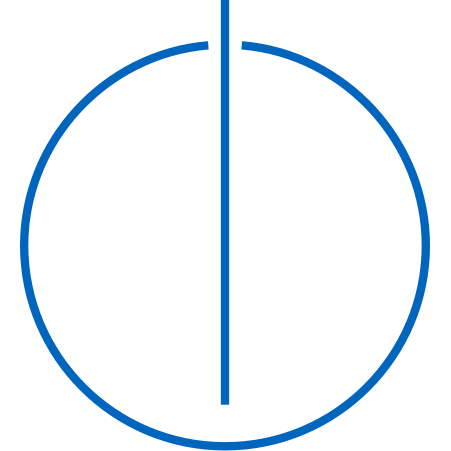
\includegraphics[height=20mm]{logos/faculty.png}
  }{}
\end{titlepage}


\frontmatter{}

\begin{titlepage}
  \centering

  \IfFileExists{logos/tum.pdf}{%
    
\includegraphics[height=20mm]{logos/tum.pdf}
  }{%
    \vspace*{20mm}
  }

  \vspace{5mm}
  {\huge\MakeUppercase{\getFaculty{}}}\\

  \vspace{5mm}
  {\large\MakeUppercase{\getUniversity{}}}\\

  \vspace{20mm}
  {\Large \getDoctype{}}

  \makeatletter
  \vspace{15mm}
  \ifthenelse{\pdf@strcmp{\languagename}{english}=0}
  {
  {\huge\bfseries \getTitle{}}

  \vspace{10mm}
  {\huge\bfseries \foreignlanguage{ngerman}{\getTitleGer{}}}
  }
  {
  {\huge\bfseries \getTitleGer{}}

  \vspace{10mm}
  {\huge\bfseries \foreignlanguage{english}{\getTitle{}}}
  }
  \makeatother

  \vspace{15mm}
  \begin{tabular}{l l}
    Author:          & \getAuthor{} \\
    Supervisor:      & \getSupervisor{} \\
    Advisor:         & \getAdvisor{} \\
    Submission Date: & \getSubmissionDate{} \\
  \end{tabular}

  \IfFileExists{logos/faculty.png}{%
    \vfill{}
    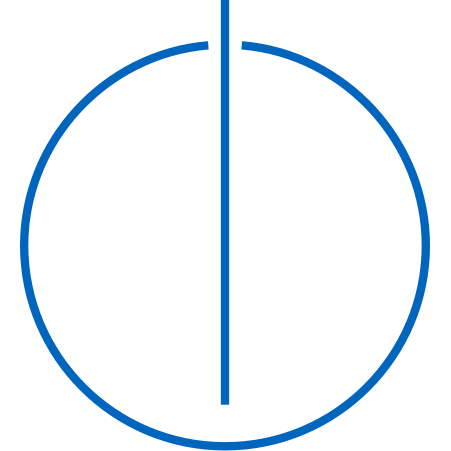
\includegraphics[height=20mm]{logos/faculty.png}
  }{}
\end{titlepage}

\cleardoublepage{}

\thispagestyle{empty}
\vspace*{0.8\textheight}
\noindent
\makeatletter
\ifthenelse{\pdf@strcmp{\languagename}{english}=0}
{I confirm that this \MakeLowercase{\getDoctype{}} is my own work and I have documented all sources and material used.}
{Ich versichere, dass ich diese \getDoctype{} selbstständig verfasst und nur die angegebenen Quellen und Hilfsmittel verwendet habe.}
\makeatother

\vspace{15mm}
\noindent
\getSubmissionLocation{}, \getSubmissionDate{} \hspace{50mm} \getAuthor{}

\cleardoublepage{}

\makeatletter
\ifthenelse{\pdf@strcmp{\languagename}{english}=0}
{\addcontentsline{toc}{chapter}{Acknowledgments}}
{\addcontentsline{toc}{chapter}{Danksagungen}}
\makeatother
\thispagestyle{empty}

\vspace*{20mm}

\begin{center}
\makeatletter
\ifthenelse{\pdf@strcmp{\languagename}{english}=0}
{\usekomafont{section} Acknowledgments}
{\usekomafont{section} Danksagungen}
\makeatother
\end{center}

\vspace{10mm}

I would like to express my sincere gratitude to Prof. Dr. Rudi Zagst from the Chair of Financial Mathematics and Prof. Dr. Martin Bichler from the Chair of Decision Sciences and Systems for giving me the chance to complete my thesis in the inter-disciplinary field of informatics and finance.

I am also extremely thankful to Michel Kschonnek %TODO: Add salutation? %  
for giving me constant support and providing me with innovative ideas. Your valuable feedback and engaging discussions were instrumental in the completion of this thesis.

Finally I would also like to extend my thanks to AllianzGI for making this project possible.



\cleardoublepage{}
 % TODO: if you don't have anyone to thank for or don't wish to publish it, comment this line out.


\makeatletter

\chapter{\abstractname}
We begin by stating the portfolio optimization problem and some of the traditional approaches used for solving it. We also mention a previous work in Reinforcement Learning (RL) and state our own project outline on how we are going to expand the work. We then start off with a short primer on RL and in particular look at an "Actor-Critic"  technique called Deep Determinisitic Policy Gradients (DDPG), which can be used to maximize rewards in a continuous setting. We state our experimental set up and also discuss  the different critic and the actor functions, we can employ in our set up. Afterwards, we then present the first version of our proposed algorithm, DDPGFunctions. We  provide a brief commentary of the system architecture of our framework, the modular components, hyper tuning framework, and the tools for tracking experiments and graphing. Understanding some potential problems with the vanilla approach we try to speed up and improve the accuracy of our results and performance in subsequent versions of DDPGFunctions - DDPGShockBuffer and DDPGEstimates. We compare our results of all these approaches against a variety of environment settings and hyper parameter configurations. In the final part of the thesis, we consider certain aspects for future work and discuss some limitations with our current approach.

% Undo the name switch
\makeatletter
\ifthenelse{\pdf@strcmp{\languagename}{english}=0}
{\renewcommand{\abstractname}{Abstract}}

\microtypesetup{protrusion=false}
\tableofcontents{}
\microtypesetup{protrusion=true}

\mainmatter{}
\chapter{Portfolio Optimization Problem}\label{chapter:PO_Problem}
In this chapter we begin by stating the Portfolio optimization problem. We then discuss some of the ways the portfolio optimization problem had been solved traditionally. We discuss some of the problems with respect to these approaches. 
We also discuss in brief some of the work done by our group in previous works.
Finally we outline our approach to solve this class of problems.

\section{Definition of the portfolio Optimization Problem} \label{section:POProblem}
We recap in this section the portfolio optimization problem as stated in an earlier work \cite{FernandezKschonnek2022}. Consider a finite time horizon $T > 0$ and a complete, filtered probability space
$(\Omega, \mathcal{F}_T , \mathbb{F} = (\mathcal{F}_{t})_{t \in [0,T]},Q)$ where the filtration $\mathbb{F}$ is generated by a Wiener process \cite{wiener1923differential} \\$W = (W(t))_{t\in[0,T]}.$\\

Consider a market model, $\mathcal{M}$ in which we have 2 assets, a risky asset which follows the Stochastic Differential Equation (SDE)

\begin{equation}
     dP_1(t) = P_1(t)(\mu dt + \sigma dW(t))
\end{equation}

 and a riskless asset which follows the SDE
 
\begin{equation}
     dP_0(t) = P_0(t)(r_c\text{ }dt).
\end{equation}

Here, $W(t)$ is the Wiener process we described earlier and the parameters $\mu$,$\sigma$ and $r_c$ are positive constants.

Let us assume that an agent in the market model specified by $\mathcal{M}$, trades in these 2 assets.  This means the agent needs to choose a portfolio process, $\pi : [0,T] \times (0,\infty) \rightarrow \mathbb{R}$, which maps the current time and the agent's current wealth $(t,v)$ to the proportion of the agent's wealth invested in the risky asset. We can state then that the evolution of the agent's wealth,$V^{v_0,\pi}$, in $\mathcal{M}$ satisfies the SDE 
\begin{equation} \label{equation:sde}
\begin{array}{l@{}l}
    dV^{v_0,\pi}(t) &{}= V^{v_0,\pi}(t) \mathbb{(}[r_c+(\mu-r_c)\pi(t,V^{v_0,\pi}(t))]dt + \pi(t,V^{v_0,\pi}(t))\sigma dW(t)\mathbb{)} \\
    V^{v_o,\pi}(0) &{}= v_0.
\end{array}
\end{equation}
Due to the Markovity of the setting, we assume that this relative portfolio process is a function of the current time and wealth $(t, V^{v_0,\pi}(t))$.
All $\pi$ satisfying some additional measurability and integrability conditions (see
equation (2.3) in \cite{Escobar-Anel2022} for details) will be called admissible and are collected in the set $\Lambda$.

We can find a semi-explicit solution for the SDE stated in (\ref{equation:sde}) as 
\begin{equation}
    V^{v_0,\pi}(t)  &{}= v_0\exp(\int_0^t r_c + (\mu-r_c)\pi(s,V^{v_0,\pi}(s)) -\frac{1}{2}(\sigma \pi ( s, V^{v_0,\pi}(s)))^2 ds
    +\int_0^t \pi(s,V^{v_0,\pi}(s))\sigma dW(s))
\end{equation}

Further, we assume that the agent is risk averse and derives utility from his terminal wealth at maturity $T$. Assume the utility function U is concave and an increasing function such that $U : [0,\infty) \rightarrow \mathbb{R} \cup \{-\infty\}$. The portfolio optimization problem is then defined as 
\begin{equation}
    (\mathbf{P})\begin{cases} \Phi(v_0) = \underset{\pi \in \Lambda}{\textit{sup }}\mathbb{ E}[U(V^{v_0,\pi}(T))]
    \end{cases}
\end{equation}

And the time-dependent version of the problem can be defined as 

\begin{equation}\label{equation:reduced_Po}
    (\mathbf{P_t}) \begin{cases}
        
     \Phi(t,v) = \underset{\pi \in \Lambda}{\textit{sup }}\mathbb{ E}[U(V^{v_0,\pi}(T)) | V^{v_0,\pi}(t)=v]
     \end{cases}
\end{equation}

There are quite a few approaches to solving this original portfolio optimization problem. We are listing some of the methods below.
\subsection{Martingale Method}
The portfolio optimization problem can be decomposed into a static optimization problem and a representation problem. The former involves determining the optimal terminal wealth, while the latter involves determining the corresponding optimal trading strategy. This approach, known as the martingale approach, is well-established in complete underlying financial market models, where it is supported by the Martingale Representation Theorem. To cite specific sources, refer to Chapter 3.4 in \cite{Korn1997} or Chapter 7.2 in \cite{Zagst2019}. However, for incomplete financial market models, such as the Heston model (see [17]), the martingale approach is not directly applicable. To address this, the financial market model can be artificially completed by adding a volatility-dependent derivative written on the risky asset, as discussed in \cite{Branger2008}, \cite{Branger2017}, \cite{Escobar2018}, and \cite{Liu2003}. 

\subsection{Merton's Method}

Merton's method of portfolio optimization \cite{Merton1969} regards the portfolio problem as a stochastic control problem, where the investor aims to maximize expected utility from consumption and terminal wealth. The method obtains the optimal value function, $\Phi (t,v)$ by solving a partial differential equation called the Hamilton-Jacobi-Bellman (HJB) equation \cite{korn2001optimal} \cite{davis1990portfolio}. The HJB equation is derived based on the principle of dynamic programming.

To solve the HJB equation, Merton's method requires an ansatz for the structure of the value function. Once the value function is obtained, the method derives the optimal trading strategy of the investor, which is a function of the portfolio's state variables - time $t$ and wealth $v$. 

\subsection{Challenges of these approaches}

The martingale approach, can be applied to characterize the optimal terminal wealth for a portfolio for many general utility functions and complete models (i.e the static problem is solvable under general assumptions) However obtaining the corresponding trading strategy (i.e solving the representation problem) is substantially more challenging in general settings.

Merton's method has the advantage of being able to handle incomplete financial models such as those with jump-diffusion processes and stochastic interest rates, but has the drawback of requiring the solution to the associated Hamilton–Jacobi–Bellman PDE. This can be challenging and time consuming especially in more complex settings, where there are no analytical solutions for this PDE.


\section{Reinforcement Learning for Portfolio Optimization and Trading Strategies}
\subsection{State of the Art}
After successes in solving games such as Atari \cite{mnih2015human}, Go, etc and also in its generic applicability to a  variety of fields such  as Natural Language Processing (NLP) (GPT models) \cite{brown2020language}, Reinforcement Learning (RL) is gaining considerable attention for its applications in finance. Several works have explored the potential of reinforcement learning techniques for financial portfolio management and trading strategies. We briefly look at some of them here.

One such work is "A deep Reinforcement learning framework for the financial portfolio management problem" by Ying et al. (2017) \cite{ying2017deep} which presents a deep reinforcement learning framework for portfolio management. They used the Deep Deterministic Policy Gradient (DDPG) algorithm, and their results showed that the proposed framework can learn effective portfolio management strategies in terms of metrics such as Sharpe ratio, portfolio returns and maximum draw down.

Another work in this field is "Application of deep reinforcement learning in stock trading strategies and stock forecasting" by Zhang et al. (2020) \cite{zhang2020application}. They proposed a deep reinforcement learning-based trading strategy that integrates technical analysis and fundamental analysis for stock trading. Their experimental results demonstrated that the proposed model can achieve better performance than other trading models in terms of the metrics such as Sharpe ratio, portfolio returns and maximum draw down.

In "Market Making via Reinforcement Learning" by Huang et al. (2018),\cite{huang2018market} the authors presented a market making algorithm that uses reinforcement learning to learn an optimal trading strategy. The algorithm is trained on a limit order book simulator and evaluated on a real-world dataset. The results showed that the algorithm can learn an effective market making strategy in terms of metrics such as effective bid-ask spread, participation rate, slippage ratio, and other portfolio metrics such as trading volume, Sharpe ratio, portfolio returns and maximum draw down etc..

Finally, "Deep Hedging" by Buehler et al. (2019) \cite{buehler2019deep} proposed a new method for hedging options in continuous time using deep learning. They demonstrated that the deep hedging approach can achieve better hedging performance than traditional methods.

\subsection{Advantages of Reinforcement Learning Techniques}
Some of the key areas where reinforcement learning techniques would fare better than traditional ways such as Merton's method and the martingale method described above are listed.
\begin{itemize}
    \item \textbf{Flexibility}: Reinforcement learning techniques can be applied to a wider range of optimization problems, without requiring assumptions on the utility functions such as concavity or differentiability.
    \item \textbf{Model-free}: Reinforcement learning techniques do not require an explicit model of the market dynamics or assumptions about the distribution of returns. This can be useful when the market model is complex and lacks analytical tractability, but can be used to sample market data efficiently.
    
   
\end{itemize}
\section{Previous Work and Project Outline}
Inspired by these advantages, previous projects in our group \cite{Janik2022} and \cite{RL_ArtInt_268}, worked on DDPG based approaches to solve this portfolio optimization problem using large neural networks to represent the "unknown" critic and actor. In that work, they obtained estimates for the Q-value function and the optimal allocation for logarithmic and power utility functions, which recovered the main characteristics of the true Q-value function and the true optimal allocation. 

However, despite achieving a reasonable estimation for the optimal allocation with both utility functions, a clear asymptotic convergence to the true optimal allocation could not be observed. Furthermore, the previous work used Tensorflow's \cite{tensorflow2015-whitepaper} implementation of DDPG and certain key parameters such as 
the magnitude of target-updates decay and (mini-) batch sizes increase during
DDPG’s run-time could not be configured. The algorithm's run time also exploded when the number of time steps in the time discretization increased.



\subsection{Project outline}
Considering the drawbacks from the previous projects, we identified the following areas of improvement, which constitute the main goals in our project.
\begin{itemize}
    \item \textbf{Specifying different function classes instead of neural networks for both Q-value and a-value function:} The motivation for moving away from an agnostic function and coming back to giving a specific structure to the functions (similar to the ansatz in Merton's method) is to incorporate known structural properties about the optimization problem into the reinforcement learning algorithm.
    \item \textbf{Build modular components:} To address the configurability problems with the previous work, we want to develop a modularized testing framework that can be utilized for different portfolio optimization problems by applying DDPG while experimenting with various specifications, such as and not limited to:
    \begin{itemize}
        \item Utility function (reward)
        \item Financial market model (environment)
        \item Parametrization of actor-function in DDPG
        \item Parametrization of critic-function in DDPG
    \end{itemize}
    \item \textbf{Tuning hyper-parameters of DDPG:}
        The framework should include a stand-alone implementation of DDPG so that changes to DDPG itself can be part of the modularization process.
    \item \textbf{Capabilities to analyze convergence speed and accuracy} 
    \item We aim to provide \textbf{detailed documentation} for the modularized testing framework so that this can be extended in future projects.
\end{itemize}




Overall, this thesis aims to develop a flexible and modular testing framework for portfolio optimization that can be adapted to various optimization problems. The performance of the DDPG algorithm in portfolio optimization will be tested under different utility functions and market models, and the results will be analyzed and compared to evaluate its accuracy and convergence speed. The framework will  be fully documented for the benefit of future users.






% !TeX root = ../main.tex
% Add the above to each chapter to make compiling the PDF easier in some editors.

\chapter{Reinforcement learning and DDPG}\label{chapter:introduction}

In this chapter we begin by giving a very short introduction of reinforcement learning (RL) and provide a taxonomy of the various flavors of RL. We then drill down to a specific branch in RL (model free, Q-Learning) that we plan to deploy for the portfolio optmization problem. We discuss these classes briefly before we move to explain the Deep Determinisitic Policy Gradients (DDPG) algorithm - the foundation for our solution. In the final part, we explain the different components of DDPG.

\section{Introduction to Reinforcement Learning}
Reinforcement learning (RL) is a field of machine learning that studies decision making in an environment, where an agent interacts with its surroundings to achieve a goal. The agent receives rewards based on the state it is in and the actions it takes. The aim is to maximize the cumulative reward over time by learning a function that maps optimal states to actions. The entire lifecycle is shown in Figure \ref{fig:rl_basic} \cite{wiki:reinforcement_learning}.

\begin{figure}[htpb]
  \centering
  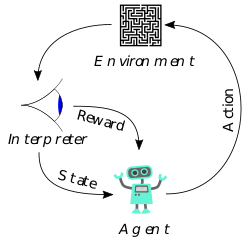
\includegraphics[width=75mm]{figures/Reinforcement_learning_diagram.png}
  \caption{Reinforcement learning} \label{fig:rl_basic}
\end{figure}

There are many flavors of RL algorithms, each targeted  at specific types of problems. A representative taxonomy of RL algorithms is provided in Figure \ref{fig:taxanomy}.

\begin{figure}[htpb]
  \centering
  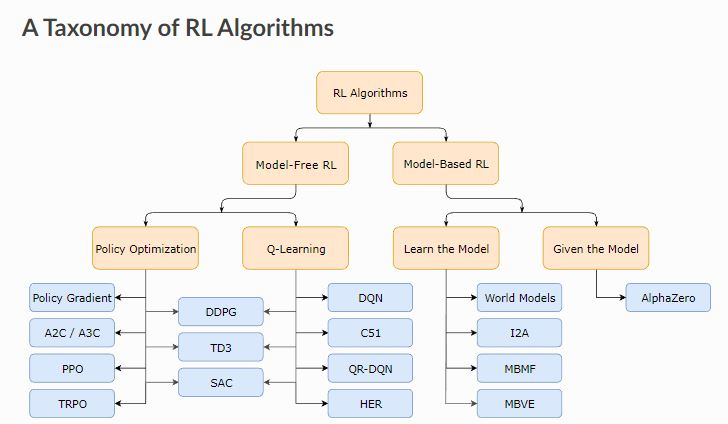
\includegraphics[width=0.8\textwidth]{figures/Taxanomy.jpg}
  \caption{Taxanomy of RL algorithms} \label{fig:taxanomy}
\end{figure}


\subsection{Model-Free vs Model-Based RL}
As can be seen in Figure \ref{fig:taxanomy}, a major classification in RL algorithms is related to the model of the environment, depending on whether or not, the model is known to the agent a priori. By model, we mean the state transition functions on taking any permissible action in the environment and also the rewards the agent obtains by taking up such an action \cite{sutton2018reinforcement}.

When the model is known to the agent, the problem is easier to solve as the agent can explicitly decide what action to take depending on the possible rewards on taking up that action. In-sample accuracy improves and training time reduces substantially when the environment can be modeled \cite{nguyen2017review}.

However in many settings, the ground truth model of the environment is  not available to the agent. 
In such cases, the agent can try to build a model based on the experience of the agent. However  such models are biased towards the training sample and quite often such agents perform terribly in real-life scenarios \cite{kaelbling1996reinforcement}.

Model-free methods on the other hand are algorithms that do not use a model of the environment, meaning they do not have a function that predicts state transitions and rewards. Instead, these methods rely solely on the experience of the agent through trial-and-error interactions with the environment. Model-free methods are easier to implement and tune compared to model-based methods, which require the agent to learn a model of the environment. Some popular model-free RL algorithms include Q-Learning, SARSA, and actor-critic networks. However, model-free methods are less sample efficient compared to model-based methods because they do not allow the agent to plan ahead. But generally they are more robust in handling real life scenarios.



\section{Q-Learning}
One of the most popular methods for solving RL problems is Q-Learning \cite{watkins1992q}, which is a model-free, off-policy algorithm. 
The basic idea behind Q-Learning is to estimate the action-value function $Q(s,a)$, also refered to as "critic", which represents the expected future reward starting from state $s$, taking action $a$ and acting optimally afterwards. The optimal action $a^*(s)$ is then computed as

\begin{equation}
a^*(s) = \arg \max_{a \in A} Q(s,a),
\end{equation}

where $A$ is the set of admissible actions.

We start off with an estimate of the $Q$ function and then iteratively update the estimate by using the Bellman optimality equation \parencite{bellman1957dynamic}


\begin{equation}
Q(s,a) \leftarrow Q(s,a) + \alpha \big[r(s,a,s') +  \max_{a' \in A} Q(s',a') - Q(s,a)\big],
\end{equation}

where $\alpha$ is the learning rate, $r(s,a,s')$ is the reward obtained after taking action $a$ in state $s$ and $s'$ is the next state.

Q-Learning has some favorable properties \cite{sutton2018reinforcement} such as:

\begin{itemize}
    \item 
    \textbf{Model-Free}: One of the key advantages of Q-Learning is that it is model free. So it is very flexible and can be applied to solve a wide range of problems.
    \item
\textbf{Off-Policy}: Q-Learning is an off-policy learner. An off-policy learner learns the value of the optimal action independently of the agent's actions. This leads to more stable results, especially when the scenarios change rapidly over time.
    \item
\textbf{Easy Implementation}: Q-Learning is a relatively simple algorithm to implement, making it a good starting point for understanding reinforcement learning.
    \item

\textbf{Good Exploration-Exploitation Trade-off}: Q-Learning balances exploration and exploitation by updating its estimates based on observed rewards. By tuning the learning rate, we can configure the exploration/exploitation trade-off at different times as we proceed into the experiment.

\end{itemize}

Q-Learning has been applied to a wide range of problems, including robot control, recommendation systems, game playing, and finance. The algorithm has been shown to be effective in many applications, but it can suffer from slow convergence and instability when applied to problems with large state spaces and sparse rewards.


One of the challenges in implementing Q-Learning is dealing with the fact that the Q-value function can have high variance. To mitigate this issue, the algorithm can be combined with function approximation techniques, such as neural networks, to approximate the value function.

\subsection{Actor - Critic Algorithm}
A variation of Q-Learning is the actor-critic algorithm \cite{konda2000actor}, which uses separate actor, $a^\phi$ and critic, $Q^\theta$ with parameters $\phi$ and $\theta$ to estimate the optimal action and the Q-value function, respectively. In other words the central underlying assumption is that $$Q(s,a) = Q^\theta(s,a)  \text{ and } a^*(s)=a^\phi(s),$$  for suitable parameterized functions $Q^\theta$ and $a^\phi$ with parameters $\theta$ and $\phi$. The actor maps states to actions, while the critic maps states and actions to a scalar value, representing the expected reward. The actor is updated based on the gradients of the Q-value function with respect to the actions, while the critic is updated using the standard Q-Learning rule. 



\section{DDPG Basics}

Deep Deterministic Policy Gradient (DDPG) is an algorithm which concurrently learns a Q-value function and an optimal action function. It uses off-policy data and the Bellman equation to learn the Q-function, and uses the Q-function to learn the policy. DDPG can only be used for environments with continuous action spaces and can be thought of as protoypical deep Q-Learning for continuous action spaces.

The DDPG approach is closely connected to Q-Learning, and is motivated by the same relation between actor $a^{\ast}$ and the critic $Q$
\begin{equation}\label{equation:Q Learning}
a^*(s) = \underset{a \in A}{\text{argmax }} Q(s,a).
\end{equation}

DDPG combines the process of learning an estimate for $Q(s,a)$ and an estimate for $a(s)$ in every update step and is tailored specifically for environments with continuous action spaces. This specialization of DDPG lies in how it calculates the maximum value of $Q(s,a)$ over all actions $a$, i.e  $\max_{a \in A} Q(s,a)$.

Finding the maximum Q-value in a scenario with a finite number of discrete actions is straightforward because we can easily evaluate the Q-values for each action and compare them, giving us the optimal action right away. However, when the action space is continuous, it's impossible to evaluate all possible actions, making the optimization problem much more complex. Using a traditional optimization algorithm to compute $\max_{a \in A} Q(s,a)$ would be computationally demanding and would have to be executed every time the agent needs to take an action, which is not practical.

Since the action space is continuous, it is assumed that the function $Q^{\theta}(s,a)$ is differentiable with respect to the action argument. This enables us to implement an efficient learning rule for the optimal action $a^\phi(s)$ that leverages this property. As a result, instead of running a costly optimization routine every time we need to calculate $\max_{a \in A} Q^\theta(s,a)$, we can approximate it as $\max_{a \in A} Q^\theta(s,a) \approx Q^\theta(s,a^\phi(s))$. 


\subsection{Algorithm}

Let us begin by stating the Bellman equation describing the optimal action-value function \cite{bellman1957dynamic} 
\begin{equation}
 Q(s,a) = \underset{s' \sim P}{{\mathbb E}}\left[r(s,a,s') +      (1-d)\max_{a'} Q(s', a')\right],   
\end{equation}


where $s' \sim P$ is shorthand for saying that the next state, $s'$, is sampled by the environment from a distribution $P(\cdot| s,a)$ and $d$ indicates whether the state $s'$ is terminal or not.

To learn an approximation of $Q(s,a)$, and $a(s)$ we use a parametrized function $Q^{\theta}(s,a)$ and $a^\phi(s)$ with parameters $\theta$ and $\phi$, and transitions $ (s,a,r,s',d)$ according to a distribution ${\mathcal D}$. We can evaluate the approximation's quality by calculating the mean-squared Bellman error (MSBE) as follows:

\begin{equation}\label{equation:Eqln}
\begin{array}{l@{}l}
L(\theta,\phi, {\mathcal D}) &{}= \underset{(s,a,r,s',d) \sim {\mathcal D}}{{\mathbb E}}\left[
    \Bigg( Q^{\theta}(s,a) - \left(r(s,a,s') +(1 - d) \max_{a'} Q^{\theta}(s',a') \right) \Bigg)^2
    \right]\\
    &{}\approx \underset{(s,a,r,s',d) \sim {\mathcal D}}{{\mathbb E}}\left[
    \Bigg( Q^{\theta}(s,a) - \left(r(s,a,s') +(1 - d) Q^{\theta}(s',a^\phi(s')) \right) \Bigg)^2
    \right]
\end{array}
\end{equation}

The Q-Learning algorithms for function approximators, including DQN and its variants as well as  DDPG, aim to minimize the MSBE loss function. These algorithms employ two key strategies and have a unique characteristic, which is specific to DDPG.

\subsubsection{Replay Buffers}

The use of an experience replay buffer is a common feature in algorithms for training deep neural networks to approximate the Q-value function, $Q(s,a)$. The replay buffer, which is a set of past experiences, must be large enough to include a diverse range of experiences, but it is important to strike a balance between having too much and too little data. Too much data may slow down the learning process, while using only the most recent data could lead to overfitting and performance issues.

It's worth noting that DDPG is an off-policy algorithm, meaning it can use experiences from outdated actions. This is possible because the Bellman equation holds for all possible transitions, regardless of how the actions were selected or what occurs after a transition. Any experiences that have been collected can be used when fitting a Q-function approximation through minimization of the mean-squared Bellman error.

\subsubsection{Target Parameters}

Several Q-Learning algorithms make use of target parameters. The term 
\begin{equation}
r(s,a,s') +(1 - d)\max_{a'} Q^{\theta}(s',a') \approx  r(s,a,s') +(1 - d) Q^{\theta}(s',a^\phi(s'))
\end{equation}
in the equation (\ref{equation:Eqln}) is called the target, because when we minimize the MSBE loss, we are trying to move the Q-value function close to this target. Q-Learning algorithms incorporate the use of target parameters to stabilize the training process. The target parameters, denoted as $\theta_{trg}$ and $\phi_{\text{trg}}$, are kept close to the actual parameters, $\theta$ and $\phi$, but with a time delay. The target parameters are used in the mean-squared Bellman error (MSBE) loss function, which is the quantity that the Q-function is trying to minimize.

To avoid instability in MSBE minimization caused by the target parameters dependence during training, the target parameters are updated periodically. In DQN algorithms, this is done by copying the actual parameters to the target every certain number of steps. In DDPG algorithms, the target parameters are obtained by weighted averaging the actual parameters and the existing target parameters with a hyperparameter $\tau$. 

\begin{equation}
\begin{array}{l@{}l}
\theta_{\text{trg}} &{}\leftarrow (1-\tau) \theta_{\text{trg}} + \tau\theta \\
\phi_{\text{trg}} &{}\leftarrow (1-\tau) \phi_{\text{trg}} + \tau\phi,

\end{array}
\end{equation}
where $\tau$ is a hyperparameter between 0 and 1 (usually close to 0). 




\subsection{Exploration vs. Exploitation}
To train the optimal allocation in DDPG, the algorithm employs an off-policy approach. To increase the exploration of previously untested actions, noise is added to the actions during training. The original DDPG paper recommends using time-correlated Ornstein-Uhlenbeck (OU) noise, but recent findings suggest that using uncorrelated, mean-zero Gaussian noise is just as effective and is simpler. It's possible to reduce the noise scale during training to improve the quality of the training data, but this is not a common practice in implementations and the noise scale is typically kept constant.

\chapter{DDPG Setup and Actor-Critic }\label{chapter:ExperimentSetup}
Before we present our version, DDPGFunctions, in this chapter we consider the broad set up for our DDPG solution. We specify the tuple - input state, action,  rewards and future states in the context of portfolio optimization. 
In the remainder of the chapter we dive deep into the actor, critic function classes  we have used in our experiments for log and power  utility functions.




\section{DDPG Setup} 
 \subsection{Recap}
 Let us first restate the portfolio optimization problem below. 
 
 \begin{equation}
    (\mathbf{P_t}) \begin{cases}
     \Phi(t,V) = \underset{\pi \in \Lambda}{\textit{sup }}\mathbb{ E}[U(V^{v_0,\pi}(T)) | V^{v_0,\pi}(t)=V]
     \end{cases}
 \end{equation}
The formulation of Q-learning is considered throughout this project, and DDPG in particular, rely on the fact that the control-process for the dynamic optimization problem is a discrete sequence of clearly separable actions \cite{RL_ArtInt_268}. As ($\textbf{P}_t$) is formulated as dynamic optimization problem with continuous-time
controls in equation (\ref{equation:reduced_Po}), we need to formulate an appropriate time-discretization version of it.

 We restrict the investor’s ability to change his relative portfolio allocation $\pi$ only at a discrete series of time-points
 $0=t_0<t_1<..<t_n=T \quad \text{with } t_i = i\frac{T}{n} = i\Delta t$\quad for i =0,...,n.    

 The set of admissible and discretized portfolio processes $\pi$ can then be characterized as    
 $$\Lambda^{\Delta t} = \Big\{\pi^{\Delta t} = (\pi_i)_{i=0,...,(n-1)} | \pi_i = \pi(t_i,\cdot) : (0,\infty) \rightarrow \mathbb{R}, \pi^{\Delta t} \in \Lambda , i=0,...,(n-1)\Big\}.$$\\
The discretized version of ($\mathbf{P}_\mathbf{t}$) can now be defined as 

 \begin{equation}\label{equation:pot}
    (\mathbf{P}^{\Delta t}_{t_i})\begin{cases} \Phi^{\Delta t}(t_i,v) = \underset{\pi \in \Lambda^{\Delta t}}{\textit{sup }}\mathbb{ E}[U(V^{v_0,\pi}(T)) | V^{v_0,\pi}(t_i)=v],\end{cases}
\end{equation}
where $\pi^{\Delta t}$ is shortened as $\pi$ for ease of exposition.
\subsection{Setup}
Given this discretized version, ($\mathbf{P}_{t_i}^{\Delta t}$) of $P_t$ we can embed ($\mathbf{P}^{\Delta t}_{t_i}$) into a deep Q-learning framework with:

\begin{itemize}
    \item The state space $S = \{t_1,..,T\} \times (0,\infty)$, where the first component is time and the second component represents investor's wealth.
    \item The action space defined as the admissible values for the relative portfolio process, i.e. $A = \mathbb{R}$.
    \item The action sequences defined as the discretized relative portfolio
processes, i.e. $a = \pi \textrm{ for } \pi \in \Lambda^{\Delta t}$
    \item The wealth updates according to a wealth update process in the continuous space as specified below.
    \begin{equation}
    \begin{array}{l@{}l}
     v_{i+1}=V^{v_0,\pi}(t_{i+1})  &{}= \underbrace{V^{v_0,\pi}(t_{i})}_{=:v_i}\exp(\int_{t_i}^{t_{i+1}} r_c + (\mu-r_c)\pi(s,V^{v_0,\pi}(s)) -\frac{1}{2}(\sigma \pi ( s, V^{v_0,\pi}(s))^2 ds \\
     &{}+\int_{t_i}^{t_{i+1}} \pi(s,V^{v_0,\pi}(s))\sigma dW(s) )\\
     &{}= v_i \exp \left ( r_c+ (\mu-r_c)\pi(t_i,v_i)  -\frac{1}{2}\left(\sigma \pi (t_i,v_i)\right)^2 \Delta t + \pi((t_i,v_i))\sigma \Delta W_{t_{i+1}}\right )
    \end{array}
    \end{equation}
    where $\Delta W_{t_{i+1}} \backsim \mathcal{N}(0,\Delta t)$
    
    Using the risky asset log returns, $\Delta P_{t_{i+1}}=ln\left(\frac{P_1(t_{i+1})}{P_1(t_{i})}\right)$, we may alternatively write$$v_{i+1} = v_{i} \exp \left ( (1-\pi(t_i,v_{i+1})r_c \Delta t+ \pi(t_i,v_i)\Delta P_{t_{i+1}}+\frac{1}{2}\sigma^2\pi(t_i,v_i)(1-\pi(t_i,v_i))\Delta t  \right)$$
    \item The reward function defined as 
    \begin{equation}
        r(s,a,s')     = r\left((t_i,v_i),\pi(t_i,v_i),(t_i+\Delta t,v_{i+1})\right)=   
                    \begin{cases}
                    0  \textrm{, if }t_i +\Delta t \neq T  \\
                    U(v_{i+1}) \textrm{, if }t_i +\Delta t = T \\
\end{cases}
    \end{equation}
    
\end{itemize}
 For setting up the actor and critic, we use specific function classes for log and power utility functions. For these functions, the true critic and the actor can be computed in closed form. We present the results in the following section.

 \section{Log Utility Function}
For the log utility function $U(v) = log(v)$, the optimal action $a^*$ (correspondingly the optimal allocation $\pi^*$) (see Remark 3.1 in \cite{FernandezKschonnek2022}) is \\

\begin{equation}\label{optimallog}
a^*(t,v) = \pi^* = \frac{\mu-r_c}{\sigma^2}.
\end{equation}

The optimal action is independent of time and wealth. Hence, rather than learning $\mu$, $r$, $\sigma$ directly, we may parametrize $a^* \approx a^{\phi}$ as

\begin{equation}\label{optimalaplog}
a^\phi(t,v) = \pi^* = \phi \quad \text{ for some } \phi \in \mathbb{R}.
\end{equation}

The value function $\Phi$ (see Remark 3.1 in \cite{FernandezKschonnek2022}) is given as

\begin{equation}\label{logUEquation}
\Phi(t,v)  = \log(v) + \left[r_c + \frac{1}{2}\left(\frac{\mu-r_c}{\sigma}\right)^2(T-t) \right]    .
\end{equation}

The Q-Value function can then be derived (see Lemma 3.4 in \cite{FernandezKschonnek2022}) as

\begin{equation}\label{OptQLog}
    \begin{array}{l@{}l}
Q(t_i,v,a) 
    &{}= \log(v) + (r_c + (\mu-r_c)a -\frac{1}{2}\sigma^2a^2)\Delta t + (r_c+\frac{1}{2}(\frac{\mu-r_c}{\sigma})^2)(T-t_{i+1}) 
   
    
\end{array}
\end{equation}
Again, rather than learning $\mu$, $r_c$, $\sigma$ directly, we can identify Q as a quadratic function in $a$ with parameters $\theta_0,\theta_1,\theta_2,\text{and } \theta_T$ such that

\begin{equation}\label{paramlog}
\begin{array}{l@{}l}
Q(t_i,v,a) = \log(v) + (\theta_0 + \theta_1a + \theta_2a^2)\Delta t + \theta_T(T-t_{i+1}).
\end{array}
\end{equation}

 \section{Power Utility Function}
For the power utility function $U(v) = \frac{1}{v}v^b$, the optimal action $a^*$ (correspondingly the optimal allocation $\pi^*$) (see Remark 3.1 in \cite{FernandezKschonnek2022}) is \\

\begin{equation}\label{optimalpow}
a^*(t,v) = \pi^* = \frac{\mu-r_c}{(1-b)\sigma^2}
\end{equation}

The optimal action is independent of time and wealth. Hence rather than learning $\mu$, $r$, $\sigma$ directly, we may parametrize $a^* \approx a^{\phi}$ as

\begin{equation}\label{optimalappow}
a^\phi(t,v) = \pi^* = \phi \quad \text{ for some } \phi \in \mathbb{R}
\end{equation}

The value function $\Phi$ (see Remark 3.1 in \cite{FernandezKschonnek2022}) is given as

\begin{equation}\label{powUEquation}
\Phi(t,v)  = \frac{1}{b}v^b \exp \left( \left(br_c + \frac{1}{2}\left(\frac{\mu-r_c}{\sigma}\right)^2\frac{b}{1-b} \right)(T-t) \right).
\end{equation}

The Q- Value function can be derived (see Lemma 3.5 in \cite{FernandezKschonnek2022}) as
\begin{multline}\label{OptQPow}
Q(t_i,v,a) = \frac{1}{b}v^b\exp\left( b\left[r_c +  \frac{(\mu-r_c)^2}{2(1-b)\sigma^2}\right](T-t_{i+1})\right) \\
\exp\left(\left\left[br_c + b(\mu-r_c)a + \frac{1}{2}b(b-1)\sigma^2 a^2)\right]\Delta t\right)
\end{multline}

Again, rather than learning $\mu$, $r_c$, $\sigma$ directly, we can identify Q as an exponentially quadratic function in $a$, with parameters $\theta_0,\theta_1,\theta_2,\text{and } \theta_T$ such that

\begin{equation}\label{parampow}
\begin{array}{l@{}l}
Q(t_i,v,a) = \frac{1}{b}v^b\exp \left( (\theta_0 + \theta_1a + \theta_2a^2)\Delta t + \theta_T(T-t_{i+1}) \right).
\end{array}
\end{equation}

 \section{Function classes for Actor and Critic}
 Based on the Q-value and a-value functions that we have defined for the utility functions, we can build different configurations of actor and critic. We summarize some of the possible configurations in Table \ref{table:actor_critic}. \\
\begin{table}
\begin{tabular}{ ||p{2cm}||p{2cm}|p{2cm}|p{2cm}|p{4cm}|p{2cm}||  } 
\hline\hline

\textbf{Case}&\textbf{Utility Function}& \textbf{Actor} & \textbf{Learnable Parameters} &\textbf{Critic}& \textbf{Learnable parameters}\\
 \hline
 (i) &Log   & $\frac{\mu-r_c}{\sigma^2}$    & None & (\ref{OptQLog})& $\mu$ and $\sigma$ \\ \hline
  (ii) &Log   & $\frac{\mu-r_c}{\sigma^2}$&$\mu$ and $\sigma$&  (\ref{OptQLog}) & $\mu$ and $\sigma$ \\
  \hline
    (iii) &Log   & $\phi$    & $\phi$  & (\ref{paramlog})& $\theta_0, \theta_1, \theta_2$ \text{ and } $\theta_T$   \\
  \hline
  (i) &Power   & $\frac{1}{1-b}\frac{\mu-r_c}{\sigma^2}$    & None & ($\ref{OptQPow}) $& $\mu$ and $\sigma$ \\
 \hline
 (ii) &Power   & $\frac{1}{1-b}\frac{\mu-r_c}{\sigma^2}$    & $\mu$ and $\sigma$ & $(\ref{OptQPow}) $& $\mu$ and $\sigma$ \\
 \hline
 (iii) &Power   & $\phi$   & $\phi$ & $(\ref{parampow}) $& $\theta_0, \theta_1, \theta_2$ \text{ and } $\theta_T$   \\
 \hline
  
\end{tabular}
\caption{\label{table:actor_critic}Actor critic functions}

 \end{table}
 
We can use the previously defined parametrizations of actor and critic derived for log and power utility functions in three natural ways:

\begin{itemize}
\item
\begin{enumerate}[(i)]
    


    \item Learn the market parameters $\mu$ and $\sigma$ through the calibration of the critic and pass them on directly to the actor
    \item Learn the market parameters $\mu$ and $\sigma$ simultaneously through the calibration of the actor and critic
    \item Learn the structural parameters $\phi,\theta_0, \theta_1, \theta_2, \text{and } \theta_T$ simultaneously through the calibration of the actor and critic 

\end{enumerate}
\item Alternatively one could still consider choosing more generic function classes, such as neural networks, in such a way that structural properties of the optimization problem are still retained. This can be very useful as many utility functions settings are complex and explicit solutions for Q functions may not be found. However we might still expect some structural form of the final solution.

    
\end{itemize}







\chapter{DDPGFunctions}\label{chapter:DDPGFuncs}
    In this chapter, we present a version of DDPG, which is implemented and set up from scratch with customizable functions for the actor and critic. We detail the pseudocode of our first version of our algorithm called DDPGFunctions and discuss the 4 main components of the algorithm
\begin{itemize}
    \item Event loop
    \item Environment
    \item Replay Buffer
    \item DDPG with actor and critic
\end{itemize}

We then summarize the methodology by going over some of the features of the algorithm.

\end{itemize}

\section{Algorithm}

There are 4 major components in the algorithm. To describe them completely, we first go over the main event loop, where the experiments progress.  We then describe the individual components in the event loop and drill deep into each one of the components to understand the whole picture.

\subsection{Event Loop}

This is the main driver of the algorithm where the agent  interacts with the environment in an episodic way. At the beginning of every episode, the agent begins with a wealth $v_0$ , and is invested in a basket of a risky and riskless asset. Based on the action learned by the agent, the allocations change over time between the 2 assets. The agent (i.e the investor) obtains a reward $r$ at the end of an episode which ends at time $T$. The goal of a whole experiment is to maximize the expected utility of the agents wealth at time $T$. The pseudo code of what happens in an episode is described below.

\begin{algorithm}
\caption{Event loop}\label{alg:eventloop}
\begin{algorithmic}[1]
\Require $total\_episodes \geq 100$
\State $ddpg \gets DDPG$
\State $actor \gets Actor $
\State $critic \gets Critic$
\State $buffer \gets ReplayBuffer$
\State $env \gets Enviroment$
\State $settings \gets Settings$
\State $ep \gets 0$
\State $noiseFactor \gets 1$
\While{$ep <= total\_episodes$}
    \State $currentState \gets env.reset$
    \While{TRUE}
    \State $action \gets actor.\phi^{actual} (currentState)$ \label{el:aN}
    \State $action \gets Policy(action,settings.NoiseScale,settings.Factor)$ \Comment{See Algorithm \ref{alg:policy}}
    \State $nextState,reward,isDone \gets env.step(currentState,action)$ \label{el:rb}
    \State $buffer.record (nextState,reward,isDone) $
    \State  $ddpg.learn()$
    \If {decayTau}
        \State $ddpg.updateTau((total\_episodes-ep)/total\_episodes)$
    \EndIf
    \If{isDone} 
        \State BREAK
    \EndIf
     \State $currentState \gets nextState$
    \State Record metrics
    \EndWhile
\EndWhile

\end{algorithmic}
\end{algorithm}
\begin{algorithm}
    \caption{Policy for optimal action}\label{alg:policy}
    \begin{algorithmic}[1]
    \Require
        \Statex $action,scale,factor \gets Action,Scale,Factor$
    \Statex
        \State $noise \gets Noise\_object$ \Comment{Could be OU or Gaussian process (config based)}
        \State  $policy\_action = action + scale*factor*noise$
        \State \Return $policy\_action$ 
    \end{algorithmic}
\end{algorithm}

Most of the pseudocode is very self explanatory. At line number \ref{el:aN}, one can see that the optimal action for the state is selected. Then, based on a policy, a certain level of noise is added to the optimal action. This controls the exploration part of the DDPG algorithm. There is a replay buffer that records all the experiences in line \ref{el:rb} (again described more in Section  \ref{subsection:replaybuffer} ). The DDPG's learning method, "learn",  then updates the optimal Q and A values for both the actual and the target network respectively. We finally record metrics to be used for tracking and visualizing results.


\subsection{Environment}
The environment itself is a custom discrete-time Black-Scholes environment with one risky-asset and bank account. The environment simulates the evolution of the investor's portfolio according to
a discrete version of the wealth SDE. The interesting function 'step' is explained in the following pseudocode.

\begin{algorithm}
\caption{Environment Step}\label{alg:env_step}
\begin{algorithmic}[1]
\Require $State,action$ 
\State $v \gets State.GetWealth()$
\State $t \gets State.GetTime()$
\State $\Delta W \gets $ Generate standard normal variable
\State $\Delta P \gets (\mu - 0.5\sigma^2)\Delta t + \sigma     \sqrt{\Delta t} \Delta W$  \label{pc:envsT:lret}
\State $v \gets v\exp{\left((1-action)r_c\Delta t + action \Delta P + \frac{1}{2}action(1-action)\sigma^2\Delta t)\right)}$\label{pc:envsT:vu}
\State $t \gets t +  \Delta t$
\State $done \gets False$ 
\If{t = T} 
    \State $reward \gets Utility(v)$
    \State $done \gets True$
\Else

    \State $reward \gets 0$
\EndIf

\State \Return $(t,v),reward,done$
\end{algorithmic}
\end{algorithm}

 At line \ref{pc:envsT:lret}, one can see the log returns of the risky asset being generated. The wealth of the portfolio is then updated at line \ref{pc:envsT:vu} ,  (see wealth dynamics, \cite{Zagst2019} [Inv. Strategies script (by Prof. Zagst) Theorem 2.18}]. The reward is only obtained at the end of the episode. For all other time steps, the reward is 0. The utility function can either be a log or power utility function in our experiments.

\subsection{Replay Buffer}\label{subsection:replaybuffer}
The replay buffer records experiences in a preset container of fixed size and evicts experiences when the buffer becomes full. The DDPG component samples random experiences from this buffer and learns the optimal Q-and a-value functions.  Each observation has to be independent of each other and the replay buffer provides a way of sampling independent observations. Otherwise, sampling the last N observations will make the observations highly correlated to each other and gradient descent would not work on those scenarios.

The replay buffer can support numerous eviction policies. Some common policies used are 

\begin{itemize}
    \item FIFO - Oldest experiences are evicted out in this policy.
    \item MRU - Most recently used experiences can be evicted out. This would give a chance to sample from unused observations by evicting out already used observations.
\end{itemize}

\subsection{DDPG}
The DDPG module is invoked by the event loop to update the value of Q and A parameters on every step.  In DDPGFunctions, the main steps of the update function are detailed in the following pseudocode.



DDPG as we have established is an off policy algorithm - in that sense, the policy that is being learned at every iteration  is not the policy used to make decisions to traverse to the next state in terms of portfolio allocation. This can be seen in the way there are 2 sets of parameters presented in the algorithm \ref{alg:ddpg_update} - actual and target. The target is in fact here, a slow moving version of the actual parameters that are both being updated at every step - $\tau$ being the factor that controls this learning. Another implementation specific comment on the algorithm is that since we do not necessarily use neural networks, we had to customize the backpropagation step of gradients by exposing an API in both the Q-value function and the a-value function, that would transmit the trainable variables. The implementation can then be generic to include any parametrized function(even a neural network) so long as we can get a list of trainable variables. 


An highlight of our implementation, is that the different modules in the update step are loosely coupled to each other - which helps us to experiment with different configurations. The critic and actor are both external to DDPG and can be the different implementations we have talked about in the Chapter \ref{chapter:ExperimentSetup}. Also, we provide hooks to have a custom actor function that can be fed in by the critic or invoke any conventional actor that can be trained.


\begin{algorithm}
\caption{DDPG Update}\label{alg:ddpg_update}
\begin{algorithmic}[1]
\State $state,action,reward,next\_state \gets ReplayBuffer.getBatch$
\State $actor \gets Actor$
\State $critic \gets Critic$

\State \\******* Update Critic  *****\\
\State $action^{target} \gets actor.\phi^{target}(next\_state)$ 
\State $Q^{target}(state,action) \gets reward + critic.Q\theta^{target}(next\_state,action^{target})$
\State $Q^{actual}(state,action) \gets critic.Q\theta^{actual}(state,action)$
\State $criticLoss \gets (Q^{target}(state,action)- Q^{actual}(state,action))^2$
\State $criticLossGradient \gets Gradient(criticLoss,critic.Trainablevariables)$
\State $ApplyGradients(criticLossGradient,critic.Trainablevariables)$

\State \\******* Update Actor  *****\\
\If{$actor.needsGradientUpdate$}
    \State $action^{actual} \gets actor.\phi^{actual}(state)$
    \State $optimalCriticValue \gets critic.Q\theta^{actual}(state,action^{actual})$
    \State $actorLoss \gets \sum_N optimalCriticValue $ \Comment{N is the minibatch size}
    \State $actorLossGradient \gets Gradient(actorcLoss,actor.Trainablevariables)$
    \State $ApplyGradients(actorLossGradient,actor.Trainablevariables)$
\Else
    \State $actor.applyCustomUpdate()$ \Comment{When parameters have to be passed into a non learnable actor }
\EndIf

\State \\******* Update Target Actor *****\\
\State $action^{target},action^{actual} \gets actor.getAllVariables$
\For {$a^{target} \in action^{target}$ and $a^{actual} \in action^{actual}$}
        \State $a^{target} = \tau a^{actual}+(1-\tau)a^{target}$
\EndFor


\State \\******* Update Target Critic  *****\\
\State $critic^{target},critic^{actual} \gets critic.getAllVariables$
\For {$c^{target} \in critic^{target}$ and $c^{actual} \in critic^{actual}$}
        \State $c^{target} = \tau c^{actual}+(1-\tau)c^{target}$
\EndFor
\end{algorithmic}
\end{algorithm}
\break


\section{DDPGFunctions - Features}

Our DDPGFunctions algorithm builds on top of the original DDPG solution with neural networks. We present a detailed analysis of the results of the algorithm in a later chapter. \label{chapter:Results} However in this brief section we comment on the features of our algorithm and the problems it is expected to solve.
\begin{itemize}
    \item \textbf{Faster simulations}: This is one of our key expectations/motivation of our algorithm. Having conventional deep layered neural network would lead to exploding run times. The problem becomes practically intractable with marginal additional complexity to the environmental set up. For example, having a 100-step simulation for 2 or more assets would by itself take weeks to converge to stable results \cite{Janik2022}. Since our functions are very simple, and the number of tunable parameters is not more than 5, convergence should be observed more rapidly.
    \item \textbf{Accurate convergence}: In most of the experiments we conducted, the problem setting is relatively simple, where the critic and the actor parametrizations are given almost explicitly the problems they are expected to solve. Thus we expect our simulations to converge to values very close to the exact results. 
    \item \textbf{Building custom deep networks}: We can still use the algorithm to build deep neural networks in settings where we cannot explicitly (analytically) specify the function for Q-and a- value functions. In these complex settings, we can still start off with a general form, which includes properties which the function are known or expected to have.  Then, we use deep neural networks for the parameters for that function. We can exploit the structural characteristics of the function while also including the advantages of having a neural network for modeling unknown properties.
\end{itemize}

\beg



 
\makeatletter
\newenvironment{breakablealgorithm}
  {% \begin{breakablealgorithm}
   \begin{center}
     \refstepcounter{algorithm}% New algorithm
     \hrule height.8pt depth0pt \kern2pt% \@fs@pre for \@fs@ruled
     \renewcommand{\caption}[2][\relax]{% Make a new \caption
       {\raggedright\textbf{\ALG@name~\thealgorithm} ##2\par}%
       \ifx\relax##1\relax % #1 is \relax
         \addcontentsline{loa}{algorithm}{\protect\numberline{\thealgorithm}##2}%
       \else % #1 is not \relax
         \addcontentsline{loa}{algorithm}{\protect\numberline{\thealgorithm}##1}%
       \fi
       \kern2pt\hrule\kern2pt
     }
  }{% \end{breakablealgorithm}
     \kern2pt\hrule\relax% \@fs@post for \@fs@ruled
   \end{center}
  }
\makeatother
\chapter{DDPG Shock Buffer}\label{chapter:ShockBuffer}
In this chapter we analyze some of the problems behind DDPGFunctions described in Chapter \ref{chapter:DDPGFuncs}. We then discuss the reasons why this could happen and ways to mitigate the problems. Afterwards, we present our 2nd version of our DDPG algorithm - DDPG Shock Buffer and explain why in this algorithm, some of the problems in DDPGFunctions get alleviated. We finally explore some hyper parameter constructs with respect to DDPG Shock Buffer and how they impact the simulations.

\section{DDPG Functions - Problems}

We noticed that while DDPG functions provided good results (we discuss them in detail in chapter \ref{chapter:Results}), sometimes we noticed the gradients explode in certain configurations. 

\begin{figure}[htpb]
\centering
  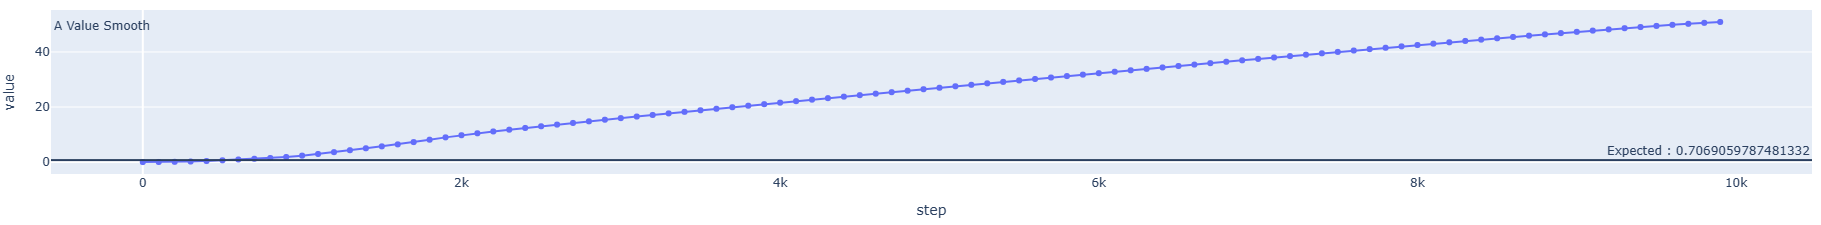
\includegraphics[width=1\textwidth,height=4cm]{figures/DDPGExplod.png}
  \caption[A value Exploding Simulations -DDPG Functions]{A-value ($a^\phi$) during training } \label{fig:expa}
\end{figure}
\begin{figure}[htpb]
\centering
  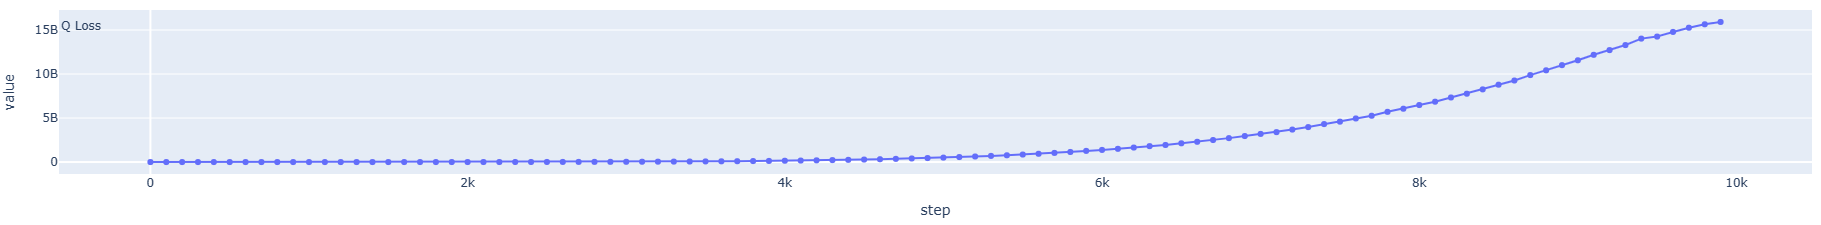
\includegraphics[width=1\textwidth,height=4cm]{figures/DDPGExplodQLoss.png}
  \caption[Q loss Exploding Simulations -DDPG Functions]{Approximate MSBE or "Q-loss" (see (\ref{equation:Eqln}))    during training } \label{fig:expqloss}
\end{figure}

    In Figures \ref{fig:expa} and  \ref{fig:expqloss}, we can see that both MSBE and a-value explode after around 800 training steps.  We saw a non trivial number of experiments (37/1404) , around 2.6\% where the gradients exploded while testing on different market parameters. In addition, we observed that for around 2.5\% of experiments the relative error between the learned portfolio allocation and the optimal allocation was more than 100\%. 


Further, we noticed that in many experiments, the variance of the learned allocation was very high during training.

\begin{figure}[htpb]
  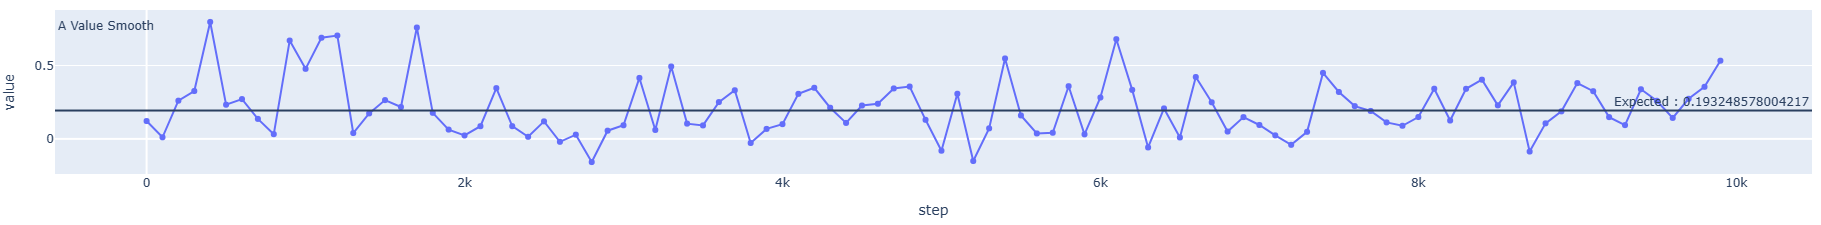
\includegraphics[width=1.0\textwidth,height=4cm]{figures/variance_ddpg.png}
  \caption[Variance of A value]{Example of high variance of $a^\phi$ during training} \label{fig:variance-ddpg}
\end{figure}

In addition to both these issues, we also wanted to explore and obtain more accurate approximation $a^\phi$ for the optimal portfolio $\pi^*$ .

\section{Key Idea}

To understand what could be a key area of improvement let us restate the Bellman optimality equation defined in Chapter \ref{chapter:PO_Problem}

\begin{equation} \label{eq:BMO1}
\begin{array}
 Q Q^*(s,a) = \underset{s' \sim P}{{\mathbb E}}\left[r(s,a,s') + (1-d) \max_{a'} Q^*(s', a')\right] \\
&\iff 0 = \left (\underset{s' \sim P}{{\mathbb E}}\left[Q^*(s,a)-r(s,a,s') - (1-d) \max_{a'} Q^*(s', a')\right] \right )^2
\end{array}
\end{equation}

The mean-squared Bellman error (MSBE) function, which tells us roughly how closely $Q^{\theta}$ comes to satisfying the Bellman equation is defined as :

\begin{equation}\label{equation:LossExpectedBM}
L(\theta,\phi, {\mathcal D}) = \underset{(s,a,r,s',d) \sim {\mathcal D}}{{\mathbb E}}\left[
    \Bigg( Q^{\theta}(s,a) - \left(r(s,a,s') +  (1 - d) \max_{a'} Q^{\theta}(s',a') \right) \Bigg)^2
    \right]
\end{equation}

In the mini batch setting which takes place in the update step of the DDPG, the expectation in Equation (\ref{equation:LossExpectedBM}) is approximated, rather than the expectation in (\ref{eq:BMO1}). Specifically DDPG uses the estimate
\begin{equation}\label{equation:bellman}
\begin{array}{l@{}l}
    &{}\underset{(s,a,r,s',d) \sim {\mathcal{D}} }{\mathbb{E}}[(r(s,a,s') + (1-d) \max_{a'} Q^\theta(s',a') - Q^\theta(s,a))^2]\\  &{} \approx \frac{1}{|\mathbi{B}|}\underset{(s,a,r,s',d) \sim {\mathbi{B}}}{\sum}(r(s,a,s') + (1-d) Q^{\theta_{trg}}(s',a^{\phi_{trg}}(s')) - Q^\theta    (s,a)))^2.
    \end{array}
\end{equation}
    where B is the mini batch and $Q^{\theta_{trg}}$ and $a^{\phi_{trg}}$ are target networks for critic and actor respectively. However, the term $s'$ is only 1 realization of the state after taking the action $a$, in state $s$. Hence, we regard the expression inside the expectation in Equation (\ref{equation:LossExpectedBM}) as a Monte-Carlo estimate for (\ref{eq:BMO1}) where just \textit{one} realization of s' is used for each state-action pair (s,a). This is bound to make the simulation unstable and may lead to the exploding gradients problem as we saw in Figure \ref{fig:expa}
We aim to mitigate this issue by obtaining more accurate estimates for the expectation in (\ref{eq:BMO1}) without requiring more samples. We contend that this should solve our exploding gradient problem and also improve our results in terms of accuracy.

\section{Algorithm}

One way of obtaining  a better estimate of the expectation in the Equation (\ref {eq:BMO1}), is to create two separate buffers $R_a$ and $R_p$. Only the observed state-action pairs $(s,a)=(t,v,a)$ are stored in $R_a$, whereas the observed one-period log-returns of the risky assets (or "shocks"), $\Delta P$, are stored in $R_p$. For given $(t,v,a) \in R_a$ and log-return $\Delta P \in R_p$, we can determine a realization of the consecutive state $s'=(t+\Delta t, V^u)$ and reward $r$ by defining
 \begin{equation}\label{equation:wu3}
    \begin{array}{l@{}l}
V^u
 &{}= V^u(v,a,\Delta P) =  V\exp{((1-a)r_c\Delta t + a\Delta P) + \frac{1}{2}a(1-a)\sigma^2\Delta t))}\\
 r(s,a,s’)  &{}= r(t_i,V^u) = \begin{cases}
                    0  \textrm{, if }t_i +\Delta t \neq T  \\
                    U(V^{u}) \textrm{, if }t_i +\Delta t = T. \\
                \end{cases}
 \end{array}
\end{equation}
In particular, as the shocks $\Delta P \in R_p$ are generated independently from $R_a$ we can sample a mini-batch $B_p \subset R_p$ to obtain a better estimate of (\ref{eq:BMO1}) for any $(s,a)=(t,v,a) \in R_a$:
\begin{equation}\label{equation:horrible}
\begin{array}{l@{}l}
&{}\left (\underset{s' \sim P}{{\mathbb E}}\left[Q(s,a)-\left(r(s,a,s') + (1-d)\max_{a'} Q(s', a')\right)\right] \right )^2\\ &{}\approx \left( Q(t,v,a) - \left(\frac{1}{|B_p|}\underset{\Delta P \in B_p}{\sum}r(t,V^u) + \mathbb{1}_{\{t+\Delta t \neq T\}}\max_{a'}(Q(t+\Delta t,V^u,a'))\right)\right)^2
\end{array}
\end{equation}
Using (\ref{equation:horrible}) and mini-batches $B_a \subset R_a$ and $B_p \subset R_p$, improve the update rule of the actor and critic parameters $\theta$ and $\phi$ to 

\begin{equation}
 \begin{array}{l@{}l}
    
\theta &{}\leftarrow  argmin_{\theta '}\frac{1}{|\mathbi{B_a}|}\underset{(t,v,a) \in B_a}{\sum}\left( Q^{\theta '}(t,v,a) - \frac{1}{|\mathbi{B_p}|}\underset{\Delta P \in B_p}{\sum} r(t,V^u) + \mathbb{1}_{\{t+\Delta t \neq T\}}  Q^{\theta_{trg}}(t+\Delta t,V^u, a^{\phi_{trg}}(t+\Delta t,V^u))\right) ^2 \\
\phi &{} \leftarrow argmax_{\phi '} \frac{1}{|{B_a}|} \underset{(t,v,a) \in B_a}{\sum} Q^{\theta}(t,v,a^{\phi '}(t,v )).
 \end{array}
  \end{equation}

The whole procedure can be explained in the following pseudo code

\begin{breakablealgorithm}
    

\caption{DDPG Shock Buffer Update}\label{alg:ddpg_shock_buffer_update}
\begin{algorithmic}[1]
\State $state_i,action_i \gets ReplayBuffer.getBatch$
\State $wealth_i,time_i  \gets state_i$
\State $dP \gets ReplayBuffer.getShockBatch$
\State $actor \gets Actor$
\State $critic \gets Critic$

\State \\******* Update Critic  *****\\

\State $wealth_{i+1} \gets wealth_i * env.wealthGridUpdate(action,dP)$ \Comment{This is a big update with $wealth_{i+1}$ dimensions being (state\_buffer\_size X shock\_buffer\_size)} \label{alg:wul}
\State $time_{i+1} \gets time_i + \Delta t$
\State $time_{i+1} \gets RepeatAcrossShockBufferSize(time_{i+1})$ \Comment{In these lines we adjust the dimension from $1 \times |m|$ to $n \times m$, where n is state\_buffer\_size and  m is shock\_buffer\_size }
\State $state_{i+1} \gets (wealth_{i+1},time_{i+1})$ \Comment{ Dimension: (state\_buffer\_size X shock\_buffer\_size)}
\State $action_{i+1} \gets aN.\Phi^{target}(state_{i+1})$ \label{alg:nal}
\If{$t_{i+1} = T$}
    \State $reward_{i+1} \gets env.U_2(wealth_{i+1})$ \label{alg:nrl1}
\Else
    \State $reward_{i+1} \gets 0 $ \label{alg:nrl}
\EndIf
\State $Q^{target}(state_{i+1},action_{i+1}) \gets reward_{i+1} + critic.Q\theta^{target}(state_{i+1},action_{i+1})$ \Comment{ Dimension: (state\_buffer\_size X shock\_buffer\_size)}

\State \\******* Arrive back at the modified Bellman optimality Equation *****\\
\State $Q^{target}(state_i,action_i) \gets getMeanAcrossShockBatch(Q^{target})$ \Comment{ Dimension: state\_buffer\_size }
\State $Q^{actual}(state_i,action_i) \gets critic.Q\theta^{actual}(state_i,action_i)$
\State $criticLoss \gets (Q^{target}(state_i,action_i)- Q^{actual}(state_i,action_i))^2$
\State $criticLossGradient \gets Gradient(criticLoss,critic.Trainablevariables)$
\State $ApplyGradients(criticLossGradient,critic.Trainablevariables)$

\State \\******* Update Actor  *****\\
\If{$actor.needsGradientUpdate$}
    \State $action_i^{actual} \gets actor.\phi^{actual}(state_i)$
    \State $optimalCriticValue \gets critic.Q\theta^{actual}(state_i,action_i)$
    \State $actorLoss \gets \sum_N optimalCriticValue $ \Comment{N is the minibatch size}
    \State $actorLossGradient \gets Gradient(actorcLoss,actor.Trainablevariables)$
    \State $ApplyGradients(actorLossGradient,actor.Trainablevariables)$
\Else
    \State $actor.applyCustomUpdate()$ \Comment{When parameters have to be passed into a non learnable actor }
\EndIf
\State \\******* Update Target Actor  *****\\
\State $action_i^{target},action_i^{actual} \gets actor.getAllVariables$
\For {$a^{target} \in action_i^{target}$ and $a^{actual} \in action_i^{actual}$}
        \State $a^{target} = \tau*a^{actual}+(1-\tau)a^{target}$
\EndFor

\State \\******* Update Target Critic  *****\\
\State $critic^{target},critic^{actual} \gets critic.getAllVariables$
\For {$c^{target} \in critic^{target}$ and $c^{actual} \in critic^{actual}$}
        \State $c^{target} = \tau*c^{actual}+(1-\tau)c^{target}$
\EndFor
\end{algorithmic}
\end{breakablealgorithm}

The main difference between Algorithm \ref{alg:ddpg_update} and Algorithm \ref{alg:ddpg_shock_buffer_update} is in  the update of the critic actor function. All the other parts of the algorithm are identical.

The most interesting aspects are at line \ref{alg:wul} where instead of 1 realization of $s'$, we have a shock\_buffer size of realizations of $s'$. Afterwards we compute the next optimal action for all these states $s'$ at line \ref{alg:nal} and the corresponding rewards at lines \ref{alg:nrl1} and \ref{alg:nrl}. We then compute the expected reward and expected Q value for the next (state,action) tuple by taking a mean over the shock buffer. We use the expected reward and the expected Q value to compute the Bellman optimality equation.

In the pseudo code at line  \ref{alg:wul}, we define the wealth update in the environment module as 

\begin{breakablealgorithm}
\caption{DDPG Wealth Update Shock Buffer}\label{alg:ddpg_shock_buffer_update_wu}
\begin{algorithmic}[1]
    \State $\mathbf{\Delta P} \gets \textrm{"Shock" returns sampled from replay buffer} R_p$ \Comment{Size : N\_s x 1 }
    \State $\textbf{a} \gets \textrm{Actions sampled from replay buffer } R_a \Comment{Size: N\_b x 1}
    \State $r,\Delta t \gets \textrm{Risk free rate, discretized time step}$
    \State \Return $\exp{\{(\mathbb{1}_{N_b} -\textbf{a})\mathbb{1}_{N_s}' r \Delta t + \textbf{a}\mathbf{\Delta P}' + \frac{1}{2}\textbf{a}(\mathbb{1}_{N_b}-\textbf{a})\mathbb{1}_{N_s}'\sigma^2 \Delta t\}}$ \Comment{$\mathbb{1}$ is a vector of all one(s) of dimension defined in subscript.  }

\end{algorithmic}    
\end{breakablealgorithm}
The environment step function is very similar to the one discussed in Chapter \ref{chapter:DDPGFuncs}, the only difference being the log return of the "shock" that is also generated is stored in a separate buffer every time a transition happens.

\subsection{Hyper Parameter Considerations}
In this very brief section, we consider the effect of the size of the shock buffer and the batch size for the shock buffer. Since the batch size of the shock buffer multiplies with the batch size of the state transitions, setting a high value for the shock buffer batch size, will increase the training times considerably. At the same time setting a low value for the shock buffer batch size will result in the same problems discussed in the original version explained in Chapter \ref{chapter:DDPGFuncs}. Hence a trade off experimentation is needed to set the optimal size of the shock buffer batch sizes.

The shock buffer size itself can be completely independent of the state buffer size. Older observations need not be discarded if the model parameters of the environment are static over time. However, in real-life scenarios, one can also think that the distribution of the log shock returns will change over time. So, having a policy like FIFO to discard the older shock observations makes sense in such settings.















\makeatletter
\newenvironment{breakablealgorithm}
  {% \begin{breakablealgorithm}
   \begin{center}
     \refstepcounter{algorithm}% New algorithm
     \hrule height.8pt depth0pt \kern2pt% \@fs@pre for \@fs@ruled
     \renewcommand{\caption}[2][\relax]{% Make a new \caption
       {\raggedright\textbf{\ALG@name~\thealgorithm} ##2\par}%
       \ifx\relax##1\relax % #1 is \relax
         \addcontentsline{loa}{algorithm}{\protect\numberline{\thealgorithm}##2}%
       \else % #1 is not \relax
         \addcontentsline{loa}{algorithm}{\protect\numberline{\thealgorithm}##1}%
       \fi
       \kern2pt\hrule\kern2pt
     }
  }{% \end{breakablealgorithm}
     \kern2pt\hrule\relax% \@fs@post for \@fs@ruled
   \end{center}
  }
\makeatother
\chapter{DDPG Estimates}\label{chapter:Estimates}
In this chapter we try to analyze some of the problems behind DDPG Shock Buffer described in Chapter \ref{chapter:ShockBuffer}. We then discuss the reasons why this could happen and ways to mitigate the problem. We then present our third version of the DDPG algorithm - DDPG Estimates and explain why in this algorithm, some of the problems in DDPG Functions get alleviated. We finally explore some hyper parameter constructs with respect to DDPG Estimates and how they can impact the simulations.

\section{DDPG Shock Buffer - Problems}

One considerable improvement of DDPG Shock Buffer over DDPG Functions was in making the simulations stable. We noticed no experiment that exploded in the calculations in that scenario (multiple market parameters for experiments up to 10 time steps). Also the number of experiments where the relative error rate was more than 100\% was around 2.06\% which was lower than DDPG Functions (we noted that such bad simulations happened when the optimal allocations were close to 0).

While the above results looked promising, we noticed that the learned optimal action $a^\phi$ still exhibits a high variance during training when using Shock Buffer, see Figure \ref{fig:sbvariance} . 

\begin{figure}[htpb]
\centering
  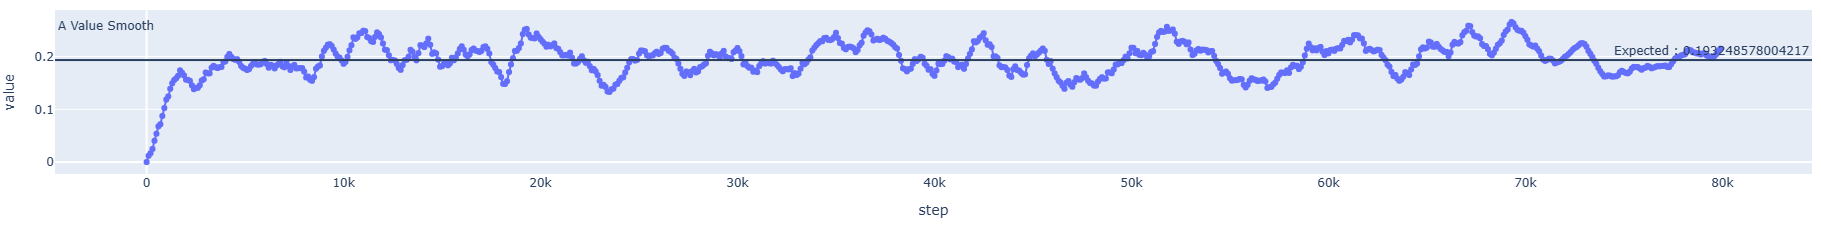
\includegraphics[width=1\textwidth,height=4cm]{figures/DDPGSBVariance.png}
  \caption[High variance Shock Buffer]{Example of high variance of $a^\phi$ during training of Shock Buffer} \label{fig:sbvariance}
\end{figure}

The other problem we faced (which also happened always with DDPG Functions) was that as the number of time steps increased, the probability that the gradients explode increased significantly. This is illustrated in Figure \ref{fig:expasb}.


\begin{figure}[htpb]
\centering
  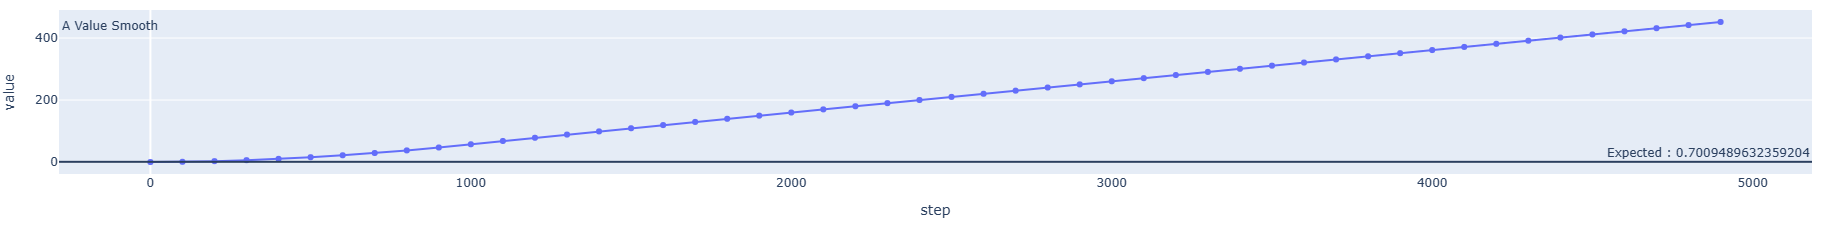
\includegraphics[width=1\textwidth,height=4cm]{figures/SBExplA.png}
  \caption[Exploding A values - Shock Buffer]{A-value ($a^\phi$)  exploding during training - Shock Buffer } \label{fig:expasb}
\end{figure}
\begin{figure}[htpb]
\centering
  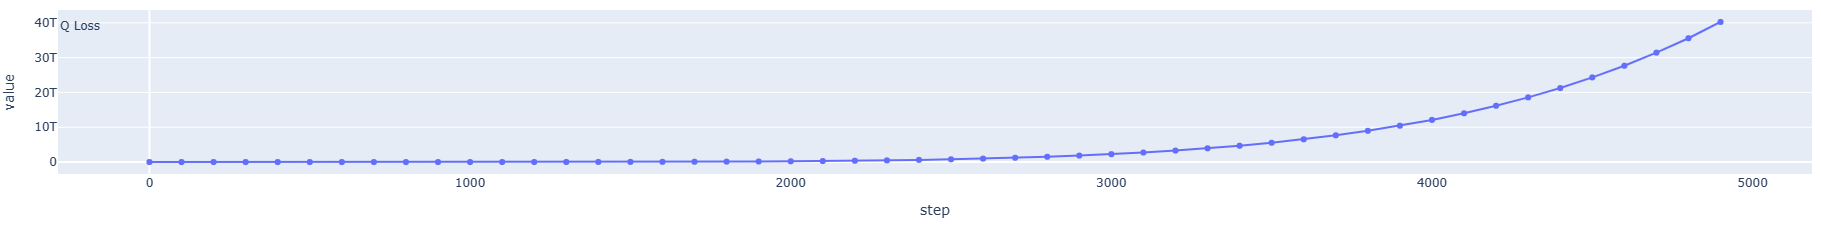
\includegraphics[width=1\textwidth,height=4cm]{figures/SBExplQ.png}
  \caption[Exploding Q loss - Shock Buffer]{Approximate MSBE or "Q-loss" (see (\ref{equation:Eqln})) exploding during training } \label{fig:expqlosssb}
\end{figure}

We noticed that the error rates could further be improved. The median accuracy we obtained for a batch of experiments was around 92\%.

\section{Key Idea}

Let us first look at some possible shortcomings in the formulation of DDPG Shock Buffer. In  DDPG Shock Buffer we strive to obtain a better estimate of the expectation defined in equation (\ref{eq:BMO1}). In DDPG Shock Buffer, this is achieved by generating multiple realizations of $s'$ on every update step by sampling from $m=|B_p|$ realizations of the past shock returns we have experienced and stored in $R_p$.

We now consider another way of obtaining  a better estimate  of the expectation defined in equation (\ref{eq:BMO1}). by using the information of the distribution of the log returns dP. Let us restate the probability density function for a standard normal distribution.
\begin{equation}\label{equation:pdf}
\varphi(x)= \frac{1}{\sqrt{(2\pi)}}e^{\frac{-x^2}{2}}
\end{equation}
Let $\beta>0$,$m \in \mathbb{N}$  and let $-\beta=z_{-n}<z_{-(n-1)}<...<z_0=0<z_1<...<z_n=\beta$ be a partition of $[-\beta,\beta]$ for large $\beta$.
Then for any (regular) $f:\mathbb{R} \rightarrow \mathbb{R}$ and $Z \sim \mathcal{N}(0,1)$
\begin{equation}\label{equation:pdf2}
\mathbb{E}[f(Z)] = \int_\mathbb{R}f(z)\varphi(z)dz \approx \int_{-\beta}^{\beta}f(z)\varphi(z) dz \approx \sum_{i=-(m-1)}^{m} f(z_i)\varphi(z_i)(z_i-z_{i-1})
\end{equation}

We can then use this idea in our framework while computing our target Q values. In our framework, the next state (i.e the next wealth) given the state $s_i = (t_i,v_i)$ and action $a_i$ can be obtained as:
\begin{equation}\label{equation:wu2}
    \begin{array}{l@{}l}
v_{i+1} 
 &{}= v_i\exp{((1-a_i)r_c\Delta t + a_i\Delta P) + \frac{1}{2}a_i(1-a_i)\sigma^2\Delta t))}\\
 &{}=: V^u(v_i,a_i,z),\\
\textrm{with, }\Delta P &{}= (\mu - \frac{1}{2}\sigma^2)\Delta t + \sigma z \sqrt{\Delta t}
\end{array}
\end{equation}
We can then use (\ref{equation:wu2}) and (\ref{equation:pdf2}) to obtain an approximate Bellman equation.

Define again the reward function $r(s,a,s')$ as 
\begin{equation}\label{rfse}
      r(s,a,s’)  &{}= r(t_i,V^u) = \begin{cases}
                    0  \textrm{, if }t_i +\Delta t \neq T  \\
                    U(V^{u}) \textrm{, if }t_i +\Delta t = T. \\
                \end{cases}
\end{equation}

Then the Bellman equation becomes
\begin{equation}
\begin{array}{l@{}l}\label{equation:sbtgtq}
Q(t,v,a)
&{}= \mathbb{E}[r(t, V^u(v,a,z))] + \mathbb{1}_{\{t+\Delta t \neq T\}} \mathbb{E}[\max_{a' \in A} Q(t+\Delta t, V^u(v,a,z),a')]\\
&{}= \int_\mathbb{R}r(t, V^u(v,a,z))\varphi(z) dz
+ \mathbb{1}_{\{t+\Delta t \neq T\}} \int_\mathbb{R}{\max}_{a' \in A} Q(t+\Delta t, V^u(v,a,z),a')\varphi(z)dz\\
&{}\approx \sum_{i=-(m-1)}^{m}[r(t, V^u(v,a,z_i))+\mathbb{1}_{\{t+\Delta t \neq T\}}\max_{a' \in A}Q(t+\Delta t, V^u(v,a,z_i),a')]\varphi(z_i)(z_i-z_{i-1})
\end{array}
\end{equation}

Thus, the core idea is to use the equation derived in (\ref{equation:sbtgtq}) in the target Q in the critic loss update step. This can be further seen in Algorithm \ref{alg:ddpg_se_iu}.


\section{Algorithm}

The procedure can be explained in the following pseudo code
\begin{breakablealgorithm}\caption{Set Initial Values} \label{alg:ddpg_se_iu}
    \begin{algorithmic}[1]
        \State $N \gets Intervals$ 
        \State $z \gets GetPartition(z)$  \label{ln:gp}
        \State $dP \gets (\mu - \frac{1}{2}\sigma^2)\Delta t + \sigma z\sqrt{\Delta t}$ for all $z$ \Comment{Dimension : N}
        \State $pdf \gets \varphi(z) =  \frac{1}{\sqrt{2\pi}}e^{-\frac{1}{2}z^2}$\Comment{Dimension : N}
        \State $diff_i \gets z_i - z_{i-1}$ for all $i$ except $i=0$,  $diff_0 \gets 0$ \Comment{Dimension : N}
        \State $dP \gets RepeatAcrossStateBufferSize(dP)$ \Comment{Dimension : state\_buffer\_size X N }
        \State $pdf \gets RepeatAcrossStateBufferSize(pdf)$ \Comment{Dimension : state\_buffer\_size X N }
        \State $diff \gets RepeatAcrossStateBufferSize(diff)$ \Comment{Dimension : state\_buffer\_size X N }
        
    \end{algorithmic}
\end{breakablealgorithm}
\pagebreak
Now the DDPG update step is explained below.

\begin{breakablealgorithm}

\caption{DDPG Estimate Update}\label{alg:ddpg_estimate_update}
\begin{algorithmic}[1]
\State $state_i,action_i \gets ReplayBuffer.getBatch$
\State $wealth_i,time_i  \gets state_i$
\State $actor \gets Actor$
\State $critic \gets Critic$

\State \\******* Update Critic  *****\\

\State $wealth_{i+1} \gets wealth_i * env.wealthGridUpdate(action,dP)$ \Comment{This is a big update with $wealth_{i+1}$ dimensions being (state\_buffer\_size X N)} \label{alg:wul3}
\State $time_{i+1} \gets time_i + \Delta t$
\State $time_{i+1} \gets RepeatAcrossNcolumns(time_{i+1})$ \Comment{Tile the next time across all partitions so the dimension lines up with $wealth_{i+1}$}
\State $state_{i+1} \gets (wealth_{i+1},time_{i+1})$ \Comment{ Dimension: (state\_buffer\_size X N)}
\State $action_{i+1} \gets aN.\phi^{target}(state_{i+1})$ \label{alg:nal3} \Comment{ Dimension: (state\_buffer\_size X N)}
\If{$t_{i+1} = T$}
    \State $reward_{i+1} \gets env.U_2(wealth_{i+1})$ \label{alg:nrl31}
\Else
    \State $reward_{i+1} \gets 0 $ \label{alg:nrl3}
\EndIf
\State $Q^{target}(state_{i+1},action_{i+1}) \gets (reward_{i+1} + critic.Q\theta^{target}(state_{i+1},action_{i+1})).pdf.diff$ \Comment{ Dimension: (state\_buffer\_size X shock\_buffer\_size) , pdf and diff are defined in algorithm \ref{alg:ddpg_se_iu}}


\State \\******* Arrive back at the modified Bellman optimality Equation *****\\
\State $Q^{target}(state_i,action_i) \gets getSumAcrossPartitionAxes(Q^{target})$ \Comment{ Dimension: state\_buffer\_size }
\State $Q^{actual}(state_i,action_i) \gets critic.Q\theta^{actual}(state_i,action_i)$
\State $criticLoss \gets (Q^{target}(state_i,action_i)- Q^{actual}(state_i,action_i))^2$
\State $criticLossGradient \gets Gradient(criticLoss,critic.Trainablevariables)$
\State $ApplyGradients(criticLossGradient,critic.Trainablevariables)$

\State \\******* Update Actor  *****\\
\If{$actor.needsGradientUpdate$}
    \State $action_i^{actual} \gets actor.\phi^{actual}(state_i)$
    \State $optimalCriticValue \gets critic.Q\theta^{actual}(state_i,action_i)$
    \State $actorLoss \gets \sum_N optimalCriticValue $ \Comment{N is the minibatch size}
    \State $actorLossGradient \gets Gradient(actorcLoss,actor.Trainablevariables)$
    \State $ApplyGradients(actorLossGradient,actor.Trainablevariables)$
\Else
    \State $actor.applyCustomUpdate()$ \Comment{When parameters have to be passed into a non learnable actor }
\EndIf
\State \\******* Update Target Actor  *****\\
\State $action_i^{target},action_i^{actual} \gets actor.getAllVariables$
\For {$a^{target} \in action_i^{target}$ and $a^{actual} \in action_i^{actual}$}
        \State $a^{target} = \tau*a^{actual}+(1-\tau)a^{target}$
\EndFor

\State \\******* Update Target Critic  *****\\
\State $critic^{target},critic^{actual} \gets critic.getAllVariables$
\For {$c^{target} \in critic^{target}$ and $c^{actual} \in critic^{actual}$}
        \State $c^{target} = \tau*c^{actual}+(1-\tau)c^{target}$
\EndFor
\end{algorithmic}
\end{breakablealgorithm}

The main difference between Algorithm \ref{alg:ddpg_update} and Algorithm \ref{alg:ddpg_estimate_update} is in  the update of the critic actor function. All the other parts of the algorithm are identical.

The most interesting aspects are at line \ref{alg:wul3} where instead of 1 realization of $s'$, we have $m$ realizations of $s'$, one realization for each grid point, $z_i$. We then compute the next optimal action for all these states $s'$ at line \ref{alg:nal3} and the corresponding rewards at line \ref{alg:nrl31} and \ref{alg:nrl3}.

In the pseudo code at line  \ref{alg:wul3}, we use the wealth update from Algorithm \ref{alg:ddpg_shock_buffer_update_wu}. The environment step function is identical to the one discussed in Chapter \ref{chapter:DDPGFuncs}. 
\subsection{Generating Intervals}
While choosing intervals stated in the Algorithm \ref{alg:ddpg_se_iu} at line \ref{ln:gp}, it is important that the discretization of the integral using "Riemann" integrals \cite{riemann1887} captures the integral approximately well. The naive way of choosing $N$ equally spaced partitions does not account for the changing size of $\varphi.$ This could in turn lead to large discretization errors in regions where $\varphi$ is large and thus cause a large error for the approximation of the integral. This can be avoided if we choose the partition in such a way that we have many grid points in regions where $\varphi$ is large and few grid points in areas where $\varphi$ is small. One such procedure is described below.

Let $\Phi$ be the cumulative distribution function of a standard normal distribution $\mathcal{N}(0,1)$, i.e
\begin{equation}
\Phi(x) = \mathbb{Pr}[Z\leq x] = \int_{-\infty}^x\varphi(z)dz.
\end{equation}
Let $F=\Phi^{-1}$ be the generalised inverse of $\Phi$, i.e the quantile function of $z  \sim \mathcal{N}(0,1)$ such that 
\begin{equation}
    X= F(\Phi(x)) = F(\mathbb{P}(Z \leq x)) \quad \forall x \in \mathbb{ R}
\end{equation}
For $m\in\mathbb{N}$, define a partition of [0,1] as
\begin{equation}
    y_j = \frac{1}{2} (1+\frac{j}{m+1}) = \frac{m+1+j}{2(m+1)} \in (0,1) \text{ for } -m \leq j \leq m
\end{equation}
Finally, we define $z_{-m}<...<z_m$ as 
\begin{equation}
    z_j = F(y_j).
\end{equation}

















\chapter{System Architecture, Design and utility frameworks}\label{chapter:SystemArchitecture}
In this chapter, we describe some highlights in terms of the architecture of the setup.  We start off by summarizing all the components we had described in Chapters \ref{chapter:DDPGFuncs}, \ref{chapter:ShockBuffer} and \ref{chapter:Estimates} with an architecture diagram and then a class diagram showing the compositional and hierarchical structure of the different classes we designed. We then proceed to give some comments about the architecture in broadly 4 areas
\begin{itemize}
    \item \textbf{Modular components of the setup}. The different components of the set up that can be 'plug and played' are.
    \begin{itemize}
        \item Actor 
        \item Critic 
        \item Replay Buffer
        \item DDPG Flavors
    \end{itemize}
    \item \textbf{Tracking , Visualization}. Combining good tracking tools such as MLFlow, we also have implemented a visualization framework based on dash \cite{dash_2022}, to see the list of results and export the data for charting, and a tailor made list of plot functions that can be extended to further projects that extend this idea.  
    \item \textbf{Deployment} - We present our Fastapi\cite{FastAPI} based server, from where experiments can be spawned directly from a webserver that can be hosted from any location.
    
    \item \textbf{Hyper parameter network}. We present a customizable tuning framework from where families of configurations can be launched from a configuration file.
    
\end{itemize}
\section{Architecture}
\begin{figure}[htpb]
\centering
  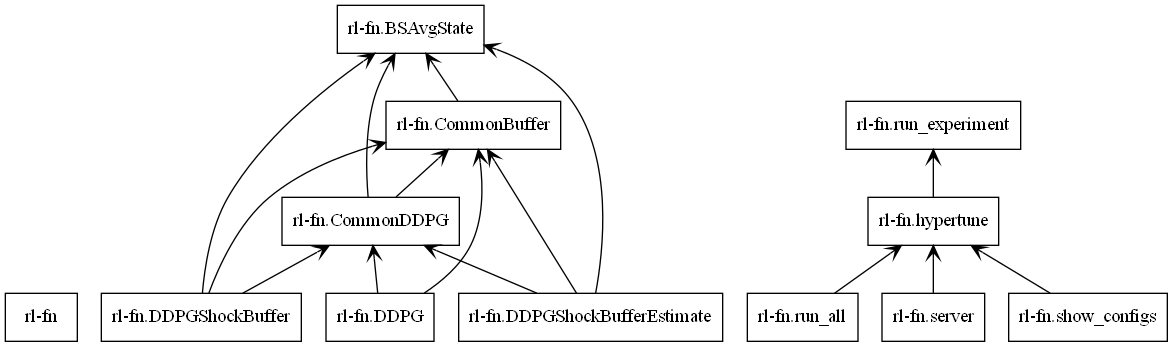
\includegraphics[width=1.0\textwidth]{figures/Results/rl-fn_architcture.png}
  \caption[Architecture]{Architecture of the different components in the project } \label{fig:architecture}
\end{figure}
There are 2 different kinds of components in the architecture specified in Figure \ref{fig:architecture} - the core DDPG components and the driver components.

The driver components broadly specify the different ways the project can be run. They are
\begin{itemize}
    \item \textbf{run\_all} : This is the traditional version of the project , a command line version from where the project can be run. The command line version takes a configuration file as input which contains the parameters of the experiments along with the hyper parameters, that have to be tuned and calls the \textbf{hypertune} component, which would spawn individual configurations for each value of a hyper parameter. The generated config would then be used by the \textbf{run\_experiment} module which would run individual experiments using the core components of the project.
    \item \textbf{server} : This is almost equivalent to the command line version in terms of the functionality but this is used while the project is hosted on a server, serving Restful APIs  \cite{fielding2000architectural} from a Flask framework \cite{UVicorn} 
    \item \textbf{show\_configs} : This version is used to only generate all the configurations, corresponding to all the tunable hyper parameters and would not run the individual experiments.  This version is ideal to inspect the possible configurations an experiment will be tuned for.
\end{itemize}
The core components encompass the different DDPG versions \textbf{DDPG}, \textbf{DDPG ShockBuffer}  and \textbf{DDPG Estimates} (shown as DDPGShockBufferEstimate in Figure \ref{fig:architecture}). The common functionalities for all these components are inherited in a \textit{base class}, \textbf{CommonDDPG}. All the 3 versions use the same replay buffer \textbf{CommonBuffer}, which is already customized to store the environment variables , extra variables such as log-returns (specific only to Shock buffer) and can be easily extended to store other parameters in any newer setting. The \textbf{BSAvgState} is the environment component that is used across all the other components and progresses the episodes of the experiments. The environment currently supports a Black-Scholes process and the utility functions - log and power. Besides the component can be extended to newer utility functions by overriding a utility interface in the environment class.   

The class diagram for these components is displayed in Figure \ref{fig:classdiag}.


\begin{figure}[htpb]
\centering
  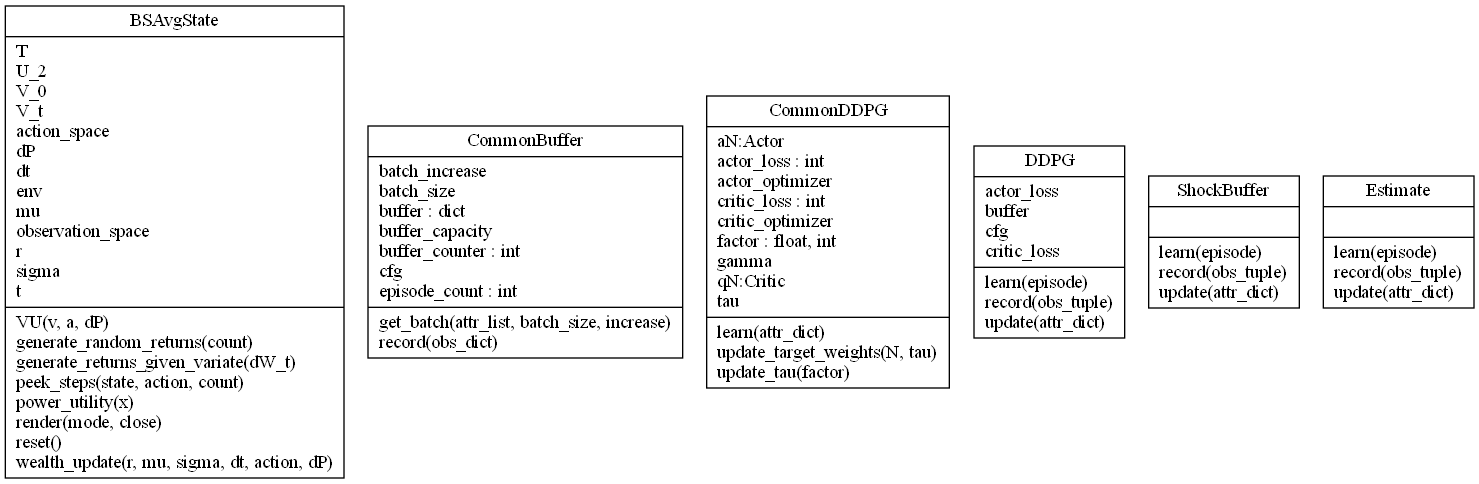
\includegraphics[width=1.0\textwidth]{figures/ClassDiagram.png}
  \caption[Class diagram]{Class diagram of DDPG components } \label{fig:classdiag}
\end{figure}
\pagebreak
Besides, we have a number of classes for the critic and the actor as well. There are 2 types of Q (and A) classes we use depending on how the critic and actor are defined. They are shown in Figure \ref{fig:classdiagc}.


\begin{figure}[htpb]
\centering
  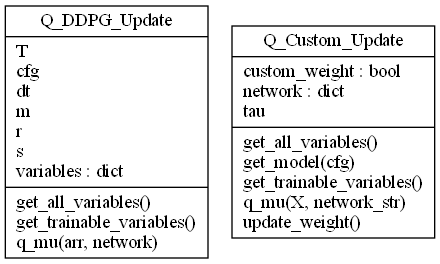
\includegraphics[width=1.0\textwidth]{figures/QClasses.png}
  \caption[Class diagram - Critic Functions]{Class diagram of critic } \label{fig:classdiagc}
\end{figure}
Q\_DDPG\_Update corresponds to cases (ii) and (iii) defined in Table \ref{table:actor_critic}, while Q\_Custom\_Update corresponds to case (i) defined in the same table.The difference between these 2 classes is that the Q\_Custom\_Update has an extra method update\_weight which needs to be customized for case (i).

\pagebreak
\section{Modular Components}\label{section:Modular Components}
At the heart of every experiment run is a configuration which we take as input.
A sample configuration is described below.
\begin{lstlisting}[language=json,firstnumber=1,caption=Example Configuration,label=json:sample_config]
{
  "name": "Experiment - Decaying tau and batch size in DDPG Shock Buffer version",
  "env": {
    "name": "BlackScholes-V2",
    "mu": 0.09,
    "sigma": 0.3,
    "r": 0,
    "T": 1,
    "dt": 0.2,
    "V_0": 1.0,
    "U_2": "pow",
    "b": -1
  },

  "general_settings": {
    "max_episodes": 5000,
    "max_steps": 100,
    "batch_size": 1024,
    "batch_size_increase": "linear"
  },
  "ddpg": {
    "type" :
       {
      "name": "DDPGShockBufferEstimate",
       "m": 20
       },
    "gamma": 1,
    "noise_decay": 1,
    "noise_scale": 1,
    "tau": 0.005,
    "tau_decay": "linear",
    "buffer_len": 20000,
    "q": {
      "name": "q_pow_utparametric",
      "lr": 0.005,
      "variables": [
        0.1,
        0.2,
        0.1,
        0.1
      ]
    },
    "a": {
      "name": "a_pow_ut1",
      "lr": 0.001,
      "variables": {
        "m": 0.1
      }
    }
  }

\end{lstlisting}

 As one can see in the Listing \ref{json:sample_config}, broadly there are 3 modules: 
 \begin{itemize}
     \item \textbf{Environment (env)}: This module takes the environment parameters, and a utility function as input. This includes $r,\mu$,$\sigma$, the time step interval $\Delta t$, T, initial wealth $v_0$ and the utility function $U$.
     
     The parameters are themselves quite flexible and new parameters can be added and existing parameters can be removed easily. For example one can set up a Heston model \cite{Heston1993}  instead of a Black Scholes Model by defining the evolution of the volatility explained by the equations
     \begin{equation}\label{HestonEq}
    \begin{array}{l@{}l}
     dS_t = (r + \eta z_t)S_tdt + \sqrt{z_t}S_tdW(t)\\
     dz_t = \kappa(\theta - z_t)dt + \sigma \sqrt{z_t}dW_z(t).     
     \end{array}
     \end{equation}
     In terms of our modular setup, we would have to redefine the step function as specified in the Algorithm \ref{alg:env_step} and then add the following variables :
     \begin{itemize}
         \item $\eta$ - Market price of the risk driver
         \item $\kappa$ - Mean reversion speed of volatility
         \item $\theta$ - Long-run average volatility
         \item $\sigma$ -  Volatility of volatility
         \item $\rho$ - Correlation factor
         
     \end{itemize} The other components of the DDPG can just 'flow' in as they were implemented.
     \item \textbf{DDPG}: 
     The DDPG module itself can be replaced by different flavors / implementation. What we described in Algorithm \ref{alg:ddpg_update} is only 1 version for our DDPG. As we have seen in Chapters \ref{chapter:ShockBuffer} and \ref{chapter:Estimates}, any DDPG model can be plugged in so long as it includes the following APIs
    \begin{itemize}
        \item Learn - The function that is meant to update the Q-value and a-value functions. 
        \item Record - The API that stores all the experience into a replay buffer.
    \end{itemize}
    Besides the APIs that DDPG should support, there are a bunch of hyper parameters that DDPG operates on, that are also listed in the sample configuration.
    \item \textbf{Actor($a$) and Critic ($Q$)}
        The different actor and critic algorithms that were discussed in detail in Chapter \ref{chapter:ExperimentSetup} are implemented in these modules. There is no restriction or a sense of constraint between the critic and the actor functions themselves. Any set of interesting modules can be used and experimented in the existing set up.
        We however require that these modules support the following APIs.
        \begin{itemize}
            \item The critic  should implement a function - Q\_mu(s,a) that returns the Q value of the state-action tuple, (s,a).
            \item The actor  should implement a function Mu(s) that returns the (suggested) optimal action for state 's'.
            \item The function TrainableVariables() for both actor and critic, that provides the list of variables to be trained using stochastic gradient descent in the context of DDPG.
            \item The function AllVariables() - A tuple of both trainable variables and the 'target' network variables that are not trained but just updated.
        \end{itemize}
 \end{itemize}
\section{Data Visualization, Experiment Tracking, Deployment and Plotting}
These are some of the downstream activities of our experiments but they are crucial to gain insights from the experiments we were conducting. Since the functions we chose for the actor and critic were quite small in terms of parameters compared to a multi-layered neural network, most of our experiments ran much faster compared to traditional DDPG problems.

Therefore we were able to run a vast number of experiments, tuning different hyper parameters, building  many versions of the core DDPG algorithm itself and also tracking the accuracy of our experiments in different environmental conditions - namely under different expected return and volatility of the risky assets.

Manually keeping track of so many experiments was hard and we were able to achieve better tracking by integrating MLFlow \cite{Zaharia2018MLflow} into our experiments. 

\subsection{Experiment Tracking and Visualization}

Here we present a dashboard that can be constructed from running many configurations in a particular experiment.

\begin{figure}[htpb]
\centering
  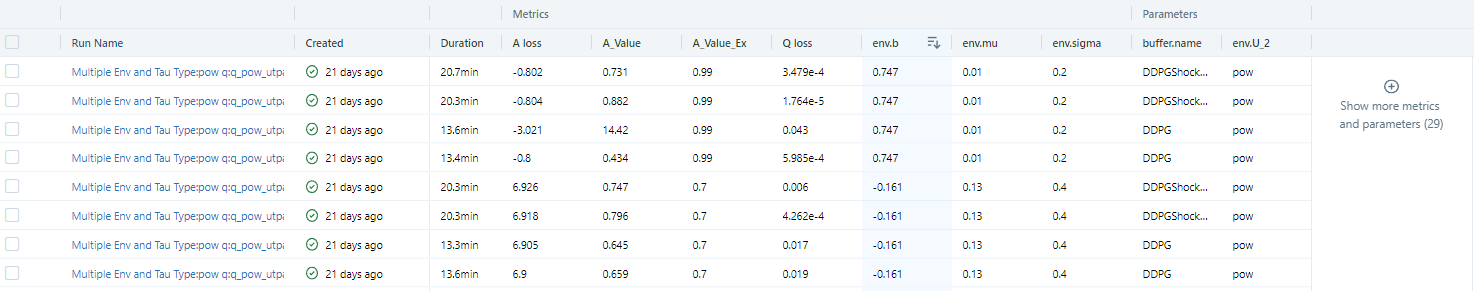
\includegraphics[width=1.0\textwidth]{figures/Dashboards.png}
  \caption[Sample Dashboard - Different Runs]{Sample dashboard showing the different runs of an experiment. Note A\_Value\_Ex is the theoretical optimal action } \label{fig:dashboard}
\end{figure}

The dashboard presents metrics, and parameters that can be logged during an experiment. Besides the metrics themselves, one can also log artifacts such as the configuration file mentioned in Listing \ref{json:sample_config}.

Within a run one can also see the progression of an experiment. The following plot shows the multi series of learned a-value, optimal a-Value, Q losses and a losses (i.e the maximization objective in the actor update) as we progress within an experiment.

\begin{figure}[htpb]
\centering
  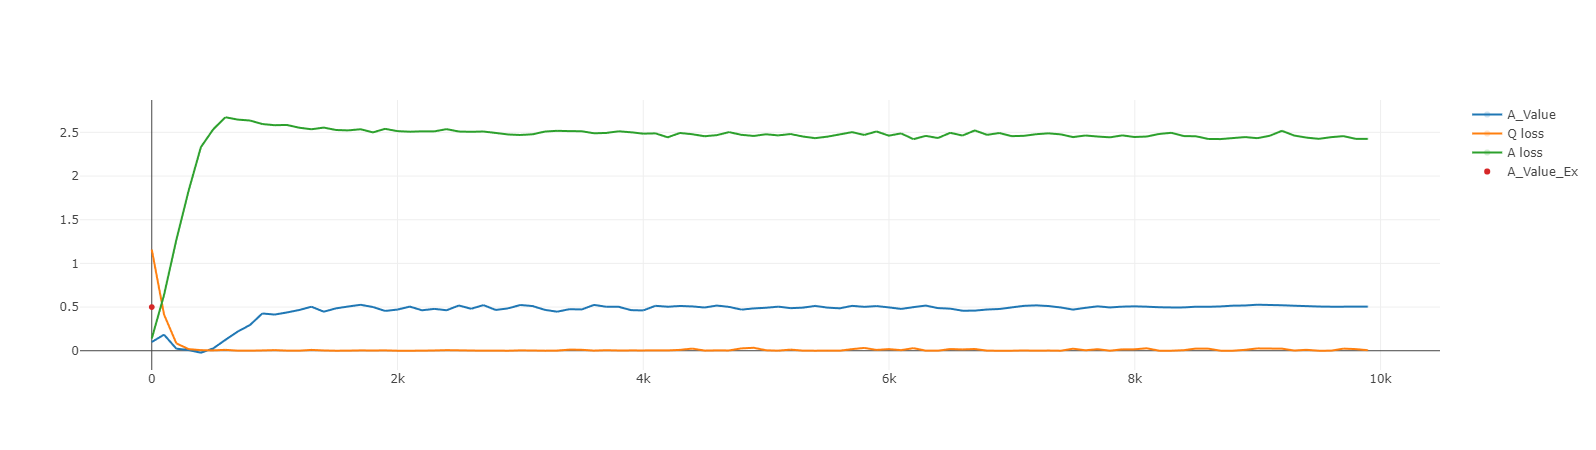
\includegraphics[width=1\textwidth,height=8cm]{figures/Losses.png}
  \caption[Sample Dashboard MLFlow]{Sample plots generated by MLFlow. } \label{fig:dashboard}
\end{figure}

Further, we also generated a customizable framework to create even more filters for our dashboards that MLFlow did not support. Our customizable framework is based on dash \cite{dash_2022} and a sample screen shot of that is found in Figure \ref{fig:DashDashboard}. We also hosted this framework at https://ddpg-po-dash1.herokuapp.com/ so that it is accessible everywhere. The difference between the framework is that the dash framework (implemented from scratch in terms of layout), has better filtering capabilities, and is much faster compared to the MLFlow UI. The layout has been improved to consider the specifics of the problem statement.
The following features are supported in the implemented dash framework in addition to the ones supported by MLFlow

\begin{itemize}
    \item Selecting multiple experiments to conduct experiments
    \item Visualizing summary statistics on the filtered experiments
    \item Visualizing losses in any particular experiment.
    \item Exporting the datatable to a comma separated value file.
\end{itemize}
Some screenshots of the application are shown in Figures \ref{fig:DashDashboard} and \ref{fig:dashboard-dash}

 \begin{figure}[!tbp]
  \subfloat[Filter ][Filter experiments]{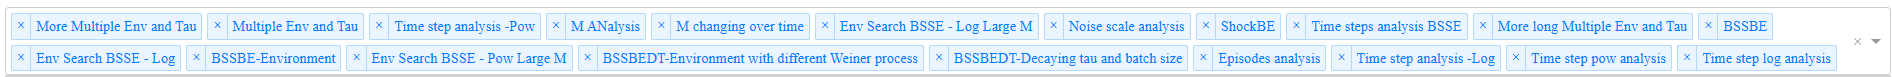
\includegraphics[width=1\textwidth]{figures/Filter.png}}
  \vfill
  \subfloat[Summary statistics ][Summary statistics]{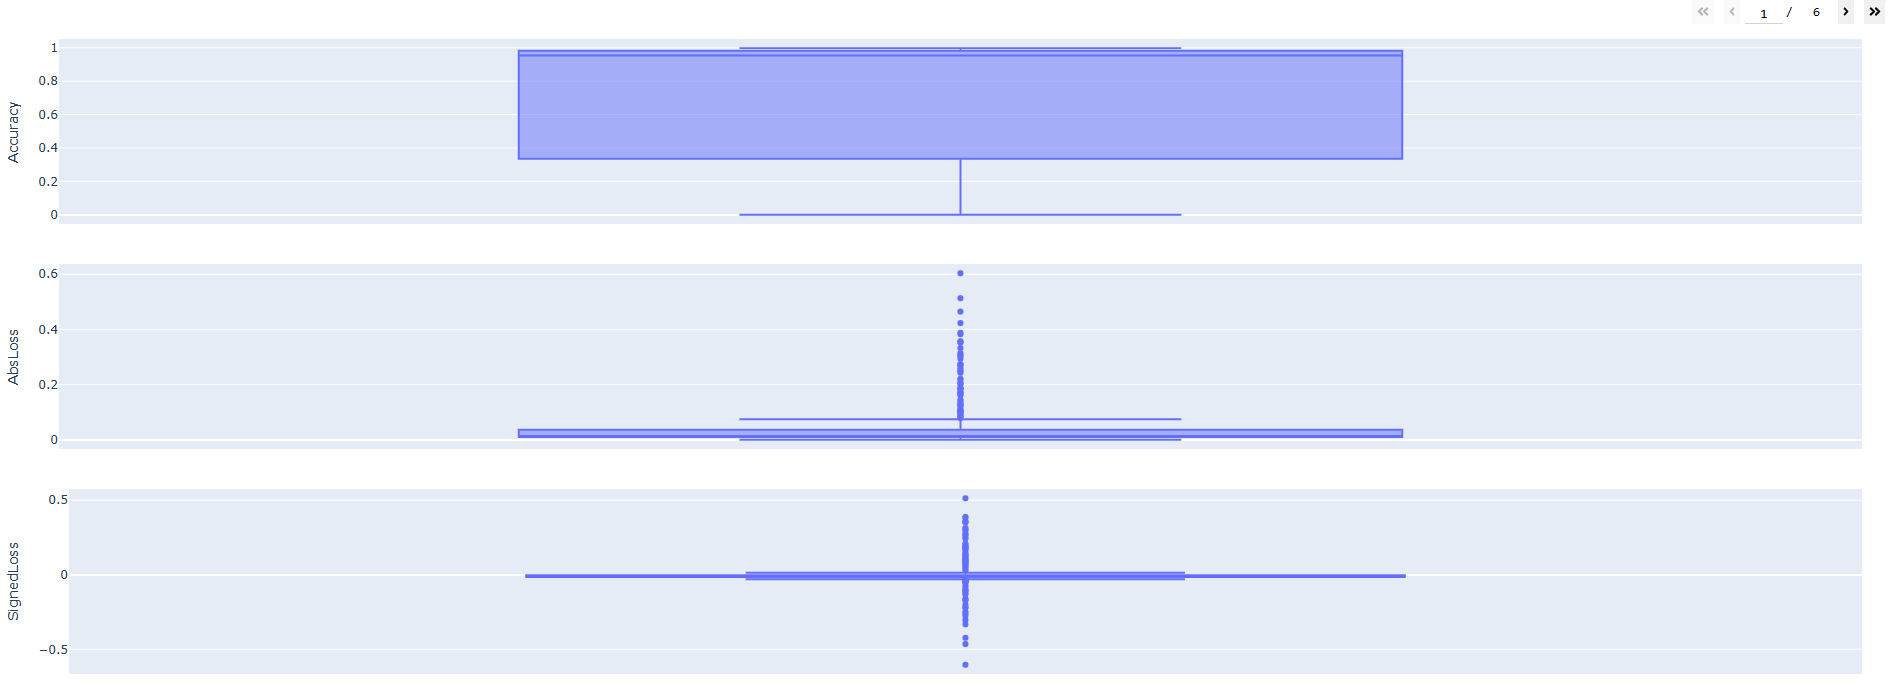
\includegraphics[width=1\textwidth,height=0.2\textheight]{figures/SS.png}}
  \vfill
  \subfloat[Losses ][Loss plots]{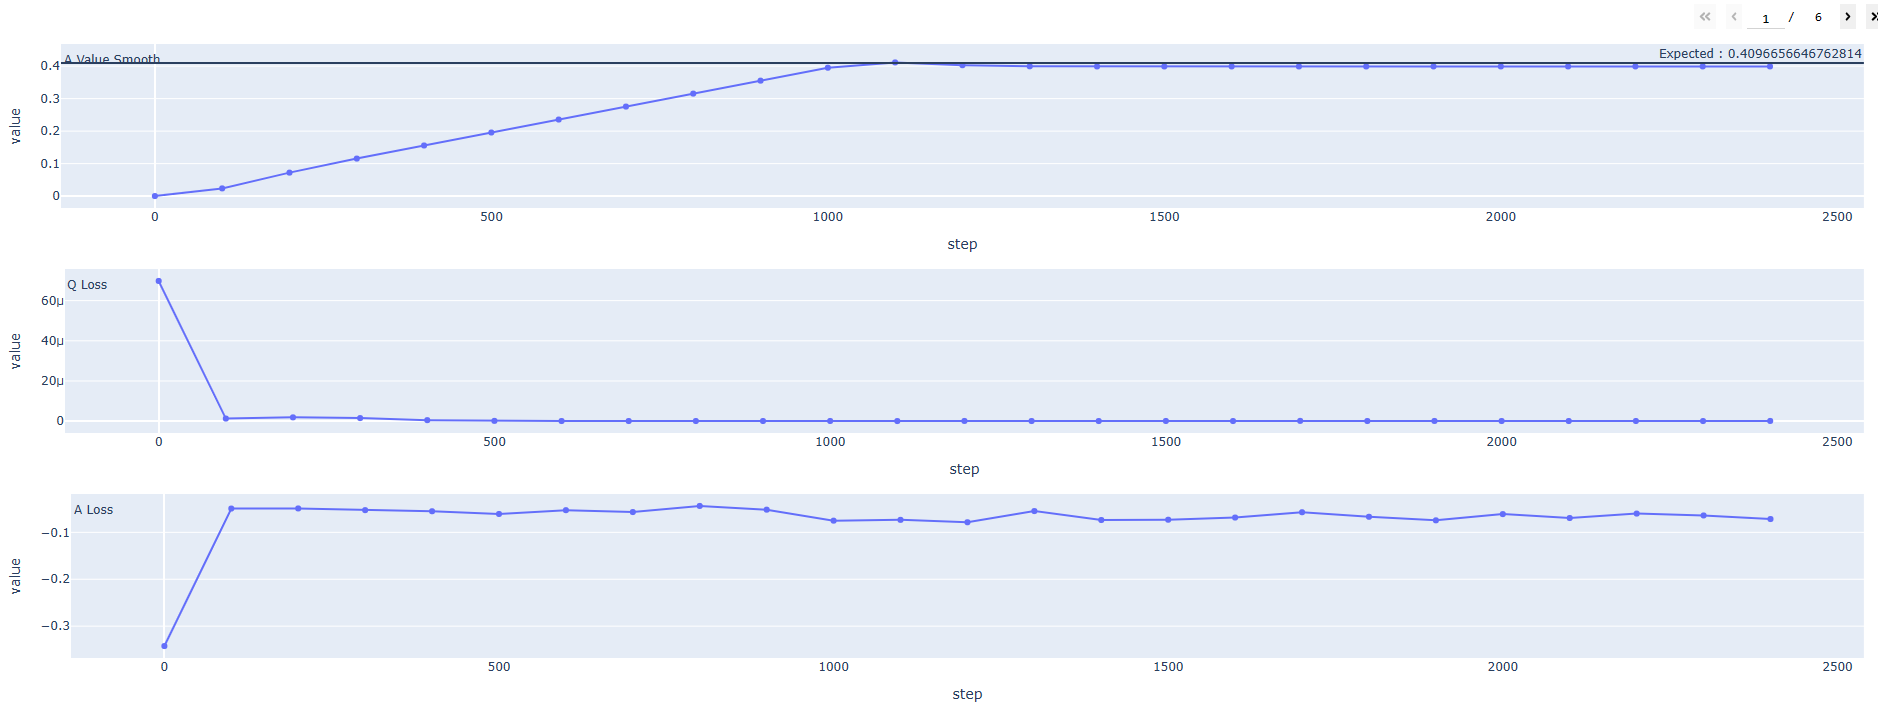
\includegraphics[width=1\textwidth,height=0.2\textheight]{figures/Plots.png}}
  \caption{ Dashboard screenshots}
  \label{fig:DashDashboard}
\end{figure}


\begin{figure}[htpb]
\centering
  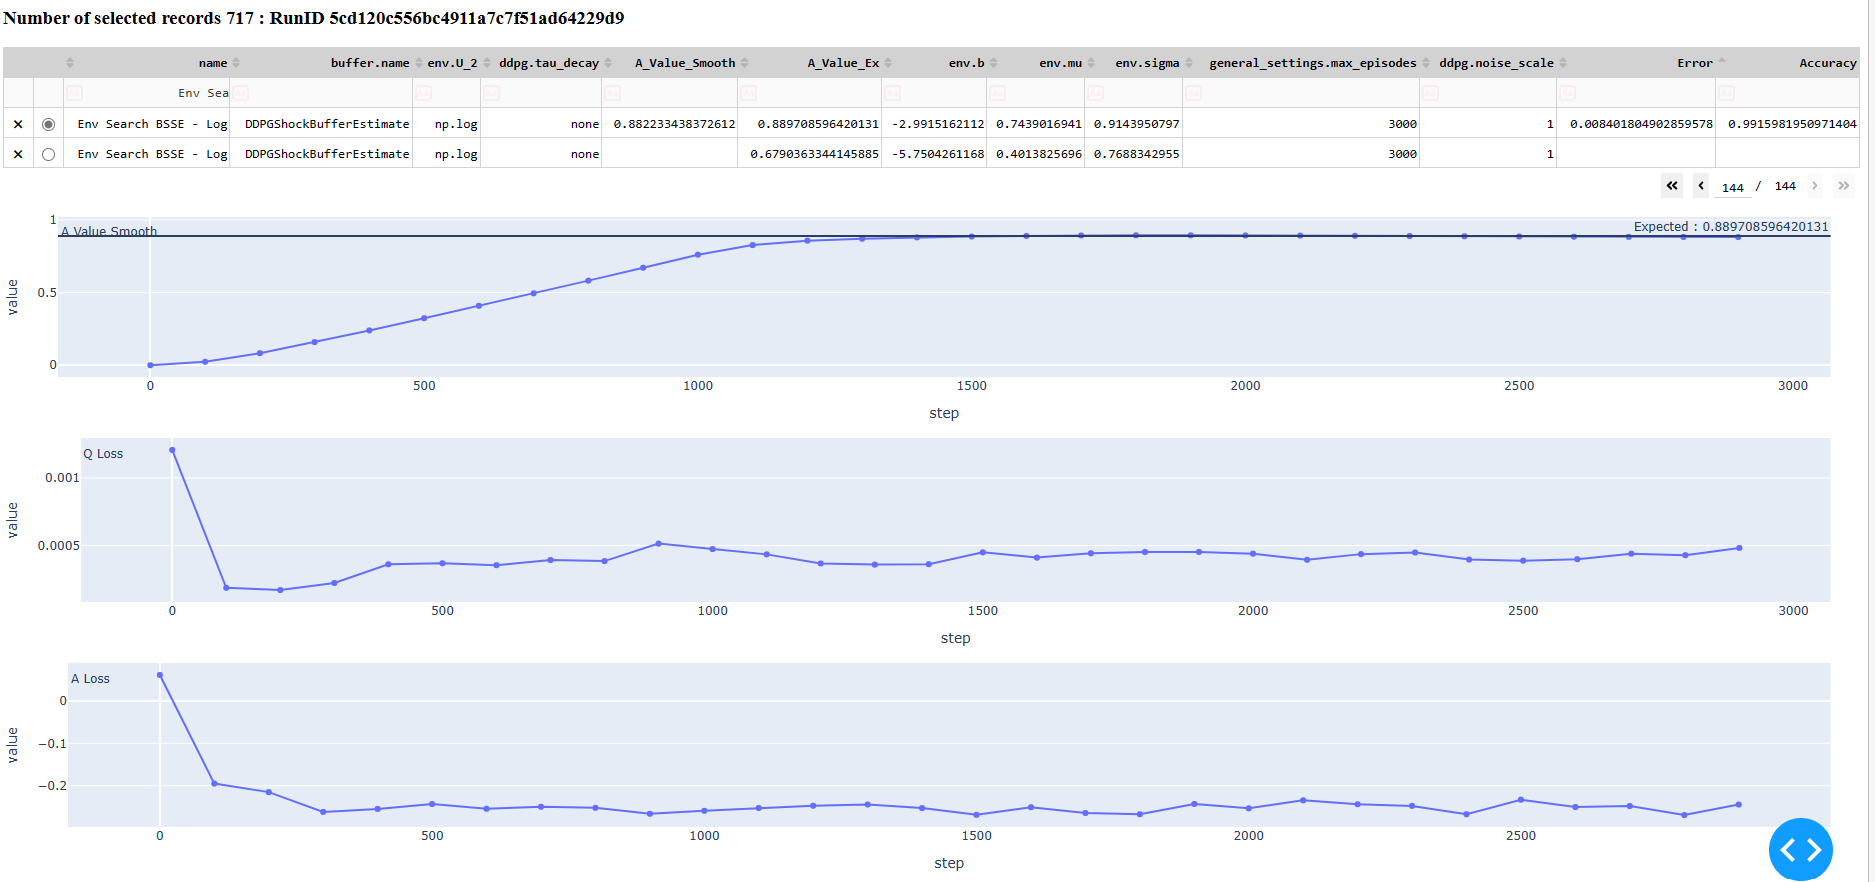
\includegraphics[width=1\textwidth,height=12cm]{figures/DashBoord-Dash.png}
  \caption[Sample plots -MLFlow Dash]{Sample plots generated by MLFlow - Dashframework} \label{fig:dashboard-dash}
\end{figure}

\pagebreak
\subsection{Deployment}
    To deploy the experiments, we implemented a framework based on the fastapi \cite{FastAPI} package. A Fastapi server is spawned using uvicorn - which is an ASGI web server implementation for Python \cite{UVicorn}. One can deploy a simple experiment or even a configuration of networks using the framework described in the next section \ref{section:hyp_parameter tuning framework}. 

    We show an experiment spawned and the resulting feedback in Figures \ref{fig:depl1} and \ref{fig:depl2}.
    
\begin{figure}[htpb]
    \centering
    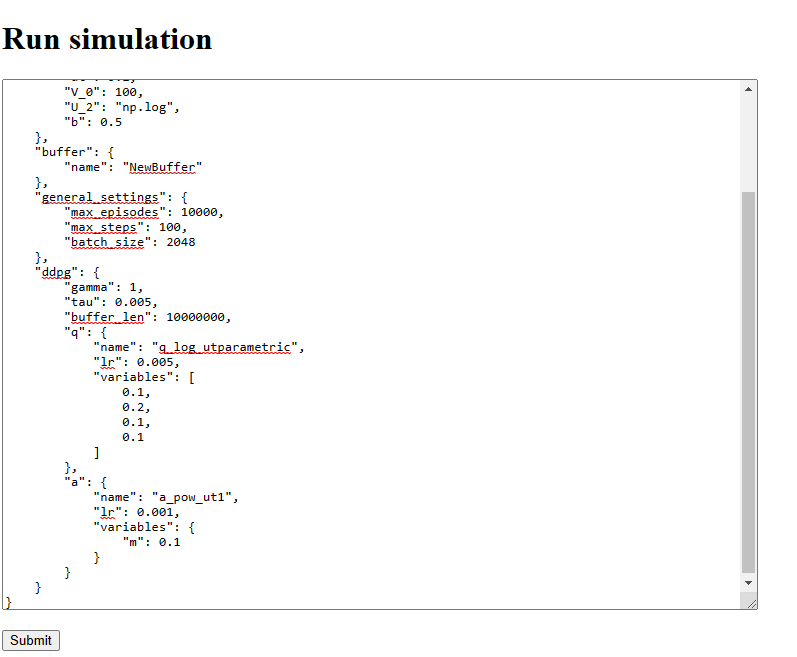
\includegraphics[width=0.5\textwidth,height=7cm]{figures/fastapi_deployment.png}
  \caption[Deployment step]{Deployment step } \label{fig:depl1}
\end{figure}
\begin{figure}[htpb]
    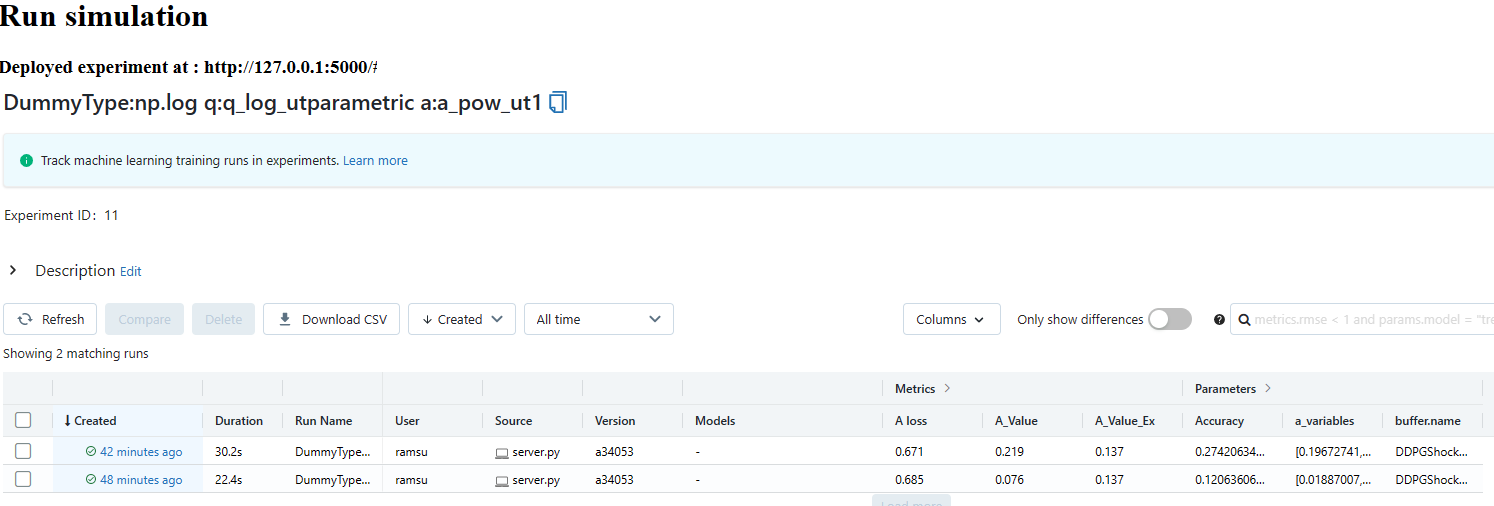
\includegraphics[width=1\textwidth,height=6cm]{figures/DeploymentResult.png}
  \caption[Deployment pipeline]{Deployment pipeline } \label{fig:depl2}
\end{figure}

\pagebreak

\section{Hyperparameter Tuning Framework} \label{section:hyp_parameter tuning framework}
One of the key requirements of the project is to conduct experiments across a large set of parameters. Some of the parameters could be environmental settings, such as the model parameters of the environment, the number of time steps to conduct an experiment, and the utility functions we need to try.

In addition, the hyper parameters of the algorithm itself could be a number of settings. For example  the parametric functions for the critic and actor, the learning rates used for the optimizing critic and actor loss, the target network learning rate $\tau$ among many others can all be changed leading to an exponential number of configurations. 

However in this section, we talk about a framework we implemented -  a configuration based approach to iterate through the different configurations of the optimization. Every base configuration specified in Listing \ref{json:sample_config} can be tuned with a tuning dictionary. A sample tuning is provided in Listing \ref{json:sample_tune_config_2}. \pagebreak
\begin{lstlisting}[language=json,firstnumber=1,caption=Tuning dictionary,label=json:sample_tune_config_2]
    "tune": {
      "buffer.name": {
        "list": [ "DDPGShockBuffer","DDPG"  ]
      },
      "env.dt" :
      {
        "list" : [ 0.01,0.02,0.1,0.2]        
      },
      "ddpg.max_episodes" :
      {
         "low" : 2000, "high" : 20000 , "step" : 100
      },
      "env.V_0"
      {
        "set" : "np.random.rand()*2" ,"size" : 10
      },
      "group":[
        {
          "env.mu": 0.019536,"env.sigma": 0.377183
        },
        {
          "env.b": -8.381621,"env.sigma": 0.57196
        }
      ],
      "group_2" :
      [
        {
        "ddpg.q.name" : "q_log_utparametric", "env.U_2" : "np.log"
        },
        {
          "ddpg.q.name" : "q_pow_utparametric","env.U_2" : "pow"
        } ]}

\end{lstlisting}
 In general every parameter specified in the configuration can be tuned. For example in the dictionary specified in 
 Listing \ref{json:sample_tune_config_2}, one of the ways the experiment can be iterated is over the time step, env.dt [See line 7]. Some of the ways the parameter can be tuned are specified below.

 \begin{itemize}
     \item \textbf{list} - By specifying list, we iterate over a set of specified values. Continuing on the example \ref{json:sample_tune_config_2} env.dt is iterated over the list { 0.01,0.02,0.1,0.2 }.
    \item \textbf{range} - By specifying the keyword,"low", and the optional parameters, "high" (default 1) and "step" (default 1) we specify a range [low,high,step] where we do a grid search for the hyper parameter from low to high incremented at each iteration by step.
    \item \textbf{set} - Set helps to evaluate an expression for the hyper parameter. The expression is any valid python based expression that returns a value compliant to the variable that it is being assigned to. In the Listing \ref{json:sample_tune_config_2}, we set $env.V_0$ the initial wealth by calling the expression "np.random.rand()*2" , 10 times.
    \item \textbf{group*} - While tuning hyper parameters, one can specify the level of granularity to iterate over by introducing "group" elements. If we do not have this element and tune over $n$ hyper parameters, then the total number of configurations generated would be $\prod_{i=1}^n C_i$ where $C_i$ is the number of values to be tested for a hyper parameter i. However, it makes sense to bunch a set of hyper parameter configurations together and iterate over another set of hyper parameters, along with them.
    
    For example, consider that we have 2 utility functions to be tested - power and log. And let the corresponding Q-value functions to be experimented are $Q^{\theta^p_i}$ and $Q^{\theta^l_j}$ respectively (where $1 \leq i \leq N_p$ and $1 \leq j \leq N_l$ ; $N_p$ and $N_l$ are positive integers). It would make sense to create a group with the power utility function and the different Q-value functions $Q^{\theta^p_i}$, and then create another group with the log utility function and  the different Q-value functions $Q^{\theta^l_j}$, instead of iterating over all possible configurations. This is possible with the "group" construct. Group elements should start with the prefix "group".
    The number of possible configurations would be $\prod_{i=1}^n G_i$ where $G_i$ is the number of configurations for a group $G_i$.  Note that  $\prod_{i=1}^n G_i \leq \prod_{j=1}^N C_j$. An element stated explicitly (as in the  examples for list, set and range)  is a group of one element trivially.
    Again within a group, one could recursively tune for list, set and range as discussed before and even have nested group variables inside it.
\end{itemize}



 
\chapter{Results}\label{chapter:Results}

In this chapter, we summarize our results comparing different DDPG algorithms specified before in Chapters \ref{chapter:DDPGFuncs} , \ref{chapter:ShockBuffer}, and \ref{chapter:Estimates}.

We first provide an overall view of the results across all the configurations we have tested. We then drill down to the performance of the algorithm under different market conditions. Some of the metrics we tested in this case are
\begin{itemize}
    \item Utility functions of wealth for the investor.
    \item Mean return ($\mu$) and volatility ($\sigma$) of the risky asset.
    \item Risk aversion factor $b$ of the investor in the case of power utility.
    \item Number of time steps (time discretization) in an episode
\end{itemize}

We proceed then to do a hyper parameter search on the tunable parameters in the different algorithms and then make inferences on the optimal hyper parameter configuration to improve our performance. Some of the hyper parameters we considered are
\begin{itemize}
\item $\tau$ -  target learning rate 
\item Noise scale to the exploration part in DDPG.
\item Number of episodes
\item Batch size
\item Number of grid points on DDPG Estimate 
\item Batch size $|B_p|=m$, for the log  returns in DDPG Shock Buffer 
\end{itemize}

We found out that in particular, Shock Buffer (Chapter \ref{chapter:ShockBuffer}) and Estimates (Chapter \ref{chapter:Estimates}) were robust and as we increased the number of sampled log returns of the shock $m$ and the number of partitions (also $m$) respectively, the accuracy also significantly increased. We repeated the experiments by increasing the number of time steps and across different model parameters for the robust version and found out that the results were stable.


\section{Performance Analysis}

We define four benchmarks  to summarize the performance analysis of our experiments. 
\begin{itemize}
    \item \textbf{Accuracy} as defined by the following equations
    \begin{equation}
        Error_{actual} = \frac{|\pi^* - a^{\phi}|}{\pi^*}
    \end{equation}
    \begin{equation}\label{equation:error}
            Error_{Normalized} = 
        \begin{cases}
          Error_{actual} \quad  Error_{actual} \leq 1 \\
          1 \quad otherwise
        \end{cases}
    \end{equation}
    \begin{equation}
        Accuracy = 1 - Error_{Normalized}.
    \end{equation}
    \item \textbf{Signed Loss} as defined by
    \begin{equation}
        Signed Loss = \pi^* - a^\phi.
    \end{equation}
    \item \textbf{Absolute Loss} as defined by
         \begin{equation}
        Absolute Loss = |\pi^* - a^\phi|.
    \end{equation}
    \item \textbf{Variance} as defined by
             \begin{equation}
                Variance = \frac{1}{100}\big {\Sigma_{i=0}^{99}} \left(a^{\phi^{(n-i)}}-\frac{1}{100}\Sigma_{j=0}^{99}a^{\phi^{(n-j)}}\right)^2,
    \end{equation}
    where $n$ is the last recent update to the algorithm
    
\end{itemize}

Going forward in this chapter, we refer to DDPG Functions, DDPG Shock Buffer and DDPG Estimates as DDPG, Shock Buffer and Estimates, respectively.
\pagebreak
\subsection{Accuracy and Losses - Overview}
We conducted a variety of experiments, with different time steps and environment parameters. The different configuration of these parameters are shown in Table \ref{table:config_overall}. In the table, Grid Points is only applicable to DDPG Estimate,  and Shock Buffer Size is only applicable to DDPG Shock  Buffer. 

\begin{table}[]
\caption{Overview configuration} \label{table:config_overall}
\begin{tabular}{||p{3cm}|p{2cm}||p{2cm}|p{2cm}||p{2cm}|p{2cm}||}
\hline
\textbf{Environment Parameter} & \textbf{Sampled values} &\textbf{DDPG}\linebreak \textbf{Parameter}& \textbf{Values} & \textbf{DDPG}\linebreak \textbf{Parameter} & \textbf{Values}\\
\hline

$\mu \in [0,1]$          & [0.07,0.955] & Version & DDPG, Shock Buffer, Estimates & Batch Size          & 1024 \\
\hline
$\sigma \in [0,1]$       & [0.1,1.4] & Grid Points &[8,1024]& Batch Size Growth & None and Linear \\
\hline
\Delta t          & [0.01,0.2] & Shock Buffer Size & [8,1024] & &\\
\hline
$v_0 \in (0,1]$        & [0.1,0.9] & Noise \linebreak  Decay       & Linear and None & & \\
\hline
Utility     & power and log & Noise \linebreak  Scale       & [0.1,5] &&  \\
\hline
$b \in [-10,1) \backslash \{0\}$ & [-9.0,0.95]  & $\tau$& $5.10^{-4}$ && \\
\hline
            T&1  &$\tau$ decay         & Linear and None && \\
\hline
            $r_c$&0  & Buffer Length     & [$10^{4}$, $10^{5}$] && \\
\hline
\end{tabular}
\end{table}



    \begin{figure}[!tbp]
  \subfloat[Box plot comparison ][Box plot comparison for all DDPG algorithms - Accuracy]{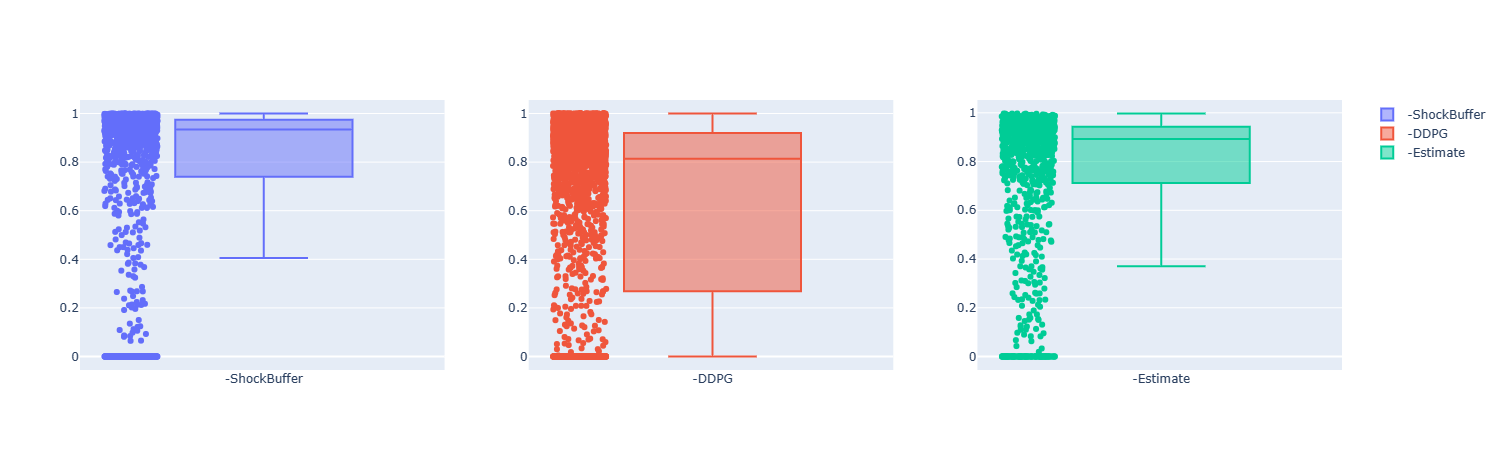
\includegraphics[width=1\textwidth,height=0.22\textheight]{figures/Results/BoxPlot_All.png}}
  \vfill
  \subfloat[Table Analysis][Tabular description of algorithms (accuracy)]{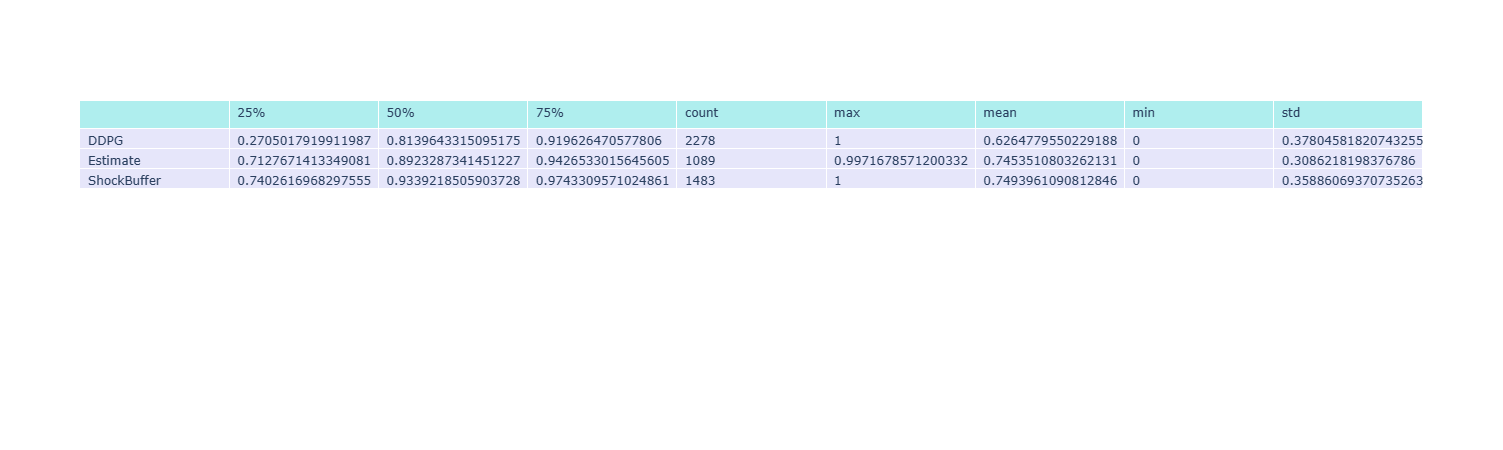
\includegraphics[width=1\textwidth,height=0.22\textheight]{figures/Results/df_BP_all.png}}
  \vfill
    \subfloat[Box plot comparison ][Box plot comparison for all DDPG algorithms - signed loss ]{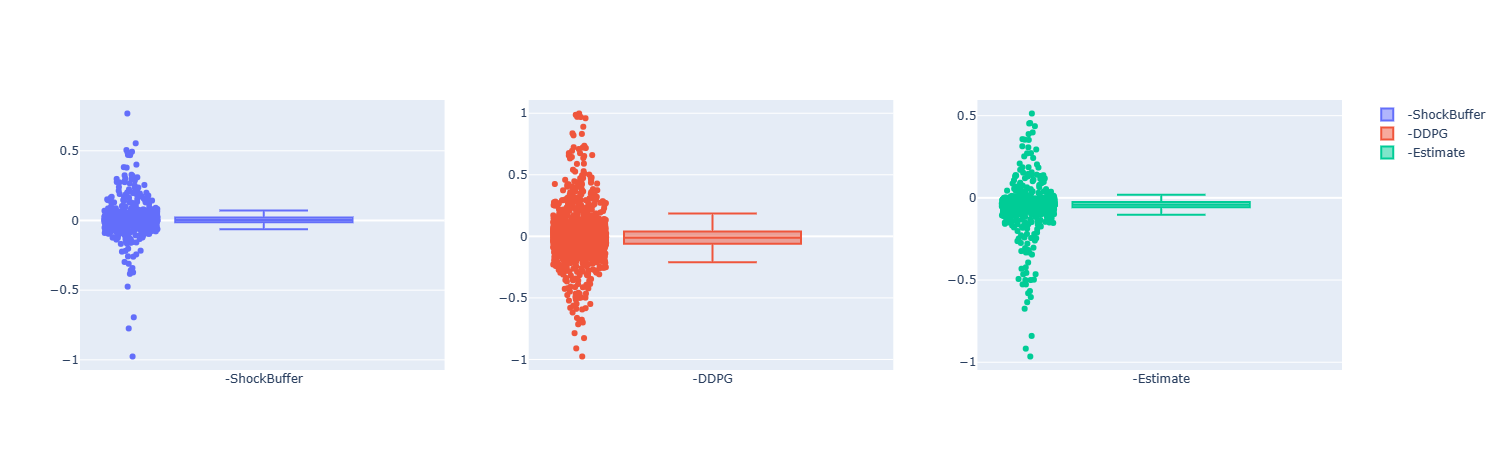
\includegraphics[width=1\textwidth,height=0.22\textheight]{figures/Results/BoxPlot_SL_All.png}}
  \vfill
  \subfloat[Table Analysis][Tabular description of algorithms (signed loss)]{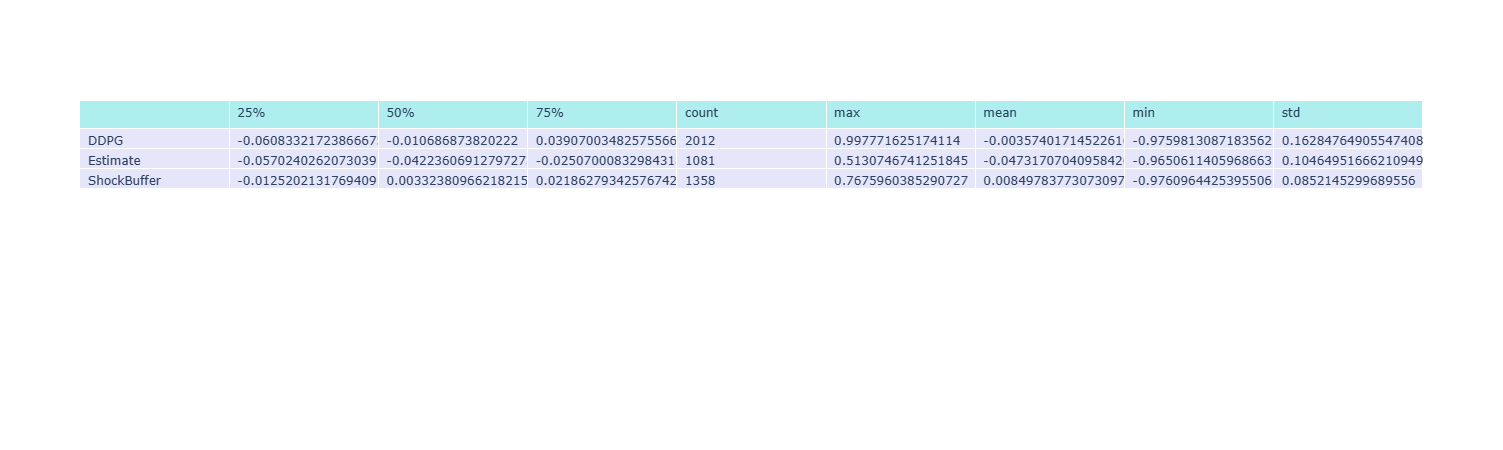
\includegraphics[width=1\textwidth,height=0.2\textheight]{figures/Results/df_BP_SL_all.png}}
  
  \caption{ Performance analysis}
  \label{fig:results:performance_analysis_all}
\end{figure}

In Figure \ref{fig:results:performance_analysis_all}, we filtered experiments, with accuracy at least greater than 0\% and removed the simulations where gradients exploded. The number of experiments were different in different versions for many reasons. Some experiments (noise scale analysis) were only conducted in 1 version of the solution (DDPG, Shock Buffer or Estimates). We started off with DDPG, and developed the other versions later so we had more experiments on DDPG compared to the rest.

From Figure \ref{fig:results:AbsAExAnalysis}, it appears that Shock Buffer and Estimates performed (in terms of accuracy) much better compared to DDPG.    All quantiles as well as the mean accuracy are higher.

Comparing Shock Buffer and Estimates, we see that Shock Buffer generally performs better. The standard deviation of accuracy for Shock Buffer is however higher compared to Estimates. In our experiments we noted that Shock Buffer simulations were quite "noisy" in convergence compared to Estimates. The sample variance in the optimal action in the experiments we conducted were lower for Estimates (2.8e-7) compared to Shock buffer (7.8e-6) at the 50th percentile.

Looking at the box plot of the signed loss in Figure \ref{fig:results:performance_analysis_all}, we see an interesting pattern for Estimates. The loss is mostly negative. which means the calculated optimal action value is lower than the optimal value. Here it seems like Estimates yields biased values for $a^*$ compared to the other versions which have a median signed loss of approximately 0.

Further, we plotted the mean absolute loss across bins of the expected optimal action constrained between 0 and 1 in Figure \ref{fig:results:AbsAExAnalysis}. 
\begin{figure}[htpb]
  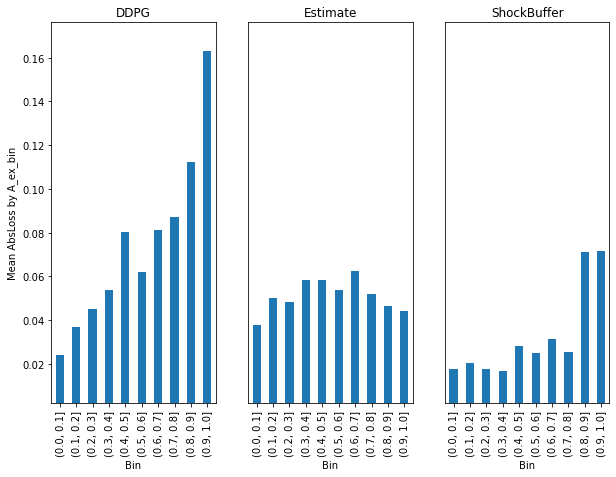
\includegraphics[width=1\textwidth,height=6cm]{figures/Results/AbsLossA_ex.png}
  \caption[Absolute loss analysis]{Absolute loss analysis} \label{fig:results:AbsAExAnalysis}
\end{figure}

In DDPG and Shock Buffer we see that as the true value of the optimal action, $a^*$  increases,  the absolute losses are much higher compared to the other intervals. However for Estimates, the absolute losses seem to be more robust in the interval [0,1].
\pagebreak

\section{Environment search}

Next we also tried to do an environment search across different model parameters and across different utility functions. The procedure for selecting the parameters is listed in Algorithm \ref{algo:EnvSearch}
\begin{algorithm}
\caption{Generate environment parameters procedure} \label{algo:EnvSearch}
\begin{algorithmic}[1]
\Require
\Statex N \Comment{Number of observations}
\Statex
\State $i \gets 0$

\While {$i<N$}
    \State $\mu \gets UniformDistribution(0,1)$
    \State $\sigma \gets UniformDistribution(0,1)$
    \State $b \gets UniformDistribution(-10,1)$
    \State  $a^*_{log} \gets \mu/\sigma^2$
    \State $a^*_{pow} \gets \mu/((1-b)\sigma^2)$
    \If {$a^*_{log} < 1$ and $a^*_{pow} < 1$}
        \State Add environment parameters \{$\mu,\sigma,b$\}
        \State $i \gets i+1$
    \EndIf
\EndWhile
\end{algorithmic}
\end{algorithm}

We sampled uniform random variables in the range [0,1] for $\mu$ and $\sigma$. For b we used a uniform distribution in the range [-10,1]. We also made sure that, expected optimal action, $a^*$ was within the range [0,1]  

The configuration for these experiments are shown in Table \ref{table:config_env}

\begin{table}[]
\caption{Configuration - Environment Analysis} \label{table:config_env}
\begin{tabular}{||p{3cm}|p{2cm}||p{2cm}|p{2cm}||p{2cm}|p{2cm}||}
\hline
\textbf{Environment Parameter} & \textbf{Sampled values} &\textbf{DDPG}\linebreak \textbf{Parameter}& \textbf{Values} &\textbf{DDPG}\linebreak \textbf{Parameter} & \textbf{Values}\\
\hline

$\mu \in [0,1]$           & \textbf{[0.07,0.955]} & Version & DDPG, Shock Buffer, Estimates & Batch Size          & 1024 \\
\hline
$\sigma\in [0,1]$        & \textbf{[0.1,1.0]} & Grid Points &20 (Estimate)& Batch Size Growth & None \\
\hline
\Delta t          & 0.2 & Shock Buffer Size & 8 (Shock Buffer)& &\\
\hline
$v_0$        & 1 & Noise \linebreak  Decay       & Linear & & \\
\hline
Utility     & power and log & Noise \linebreak  Scale       & 1 &&  \\
\hline
$b \in [-10,1) \backslash \{0\}$ & [-9,0.95]  & $\tau$& $5.10^{-4}$ && \\
\hline
            T&1  &$\tau$ decay         & Linear && \\
\hline
            $r_c$&0  & Buffer Length     & $10^{4}$ && \\
\hline
\end{tabular}
\end{table}


The results are shown in Figures \ref{fig:results:AHMPU}, \ref{fig:results:AHMLU} and \ref{fig:results:AHMA}. The lower triangle in these plots is empty because of the way the parameters were chosen with the constraint on optimal action values, $a^*$ being in [0,1].

\begin{figure}[htpb]
  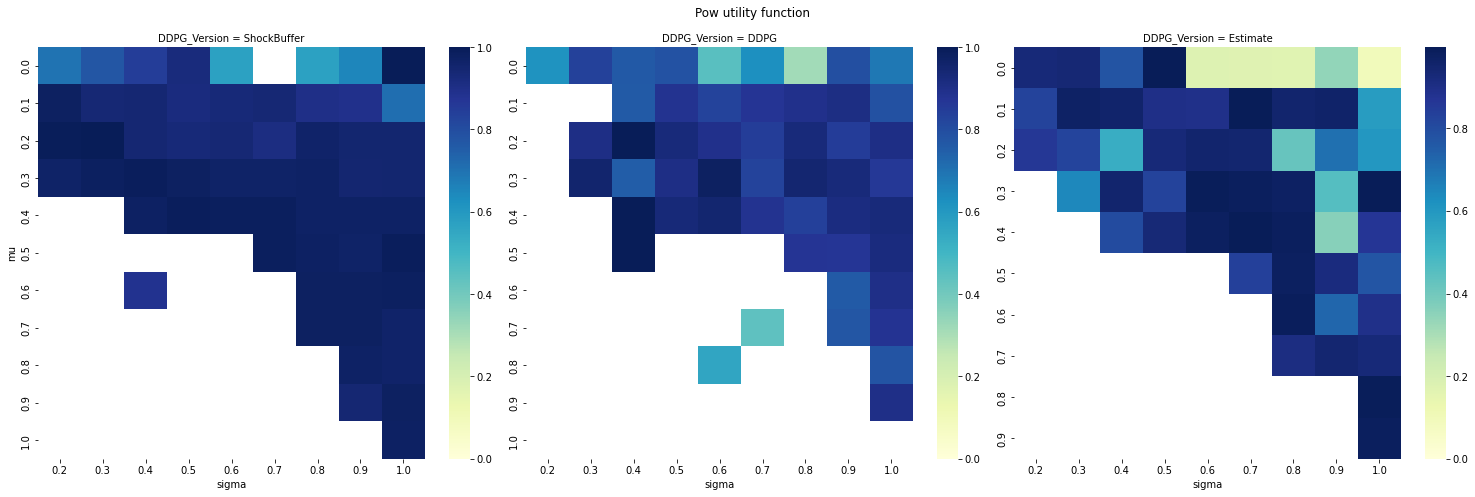
\includegraphics[width=1\textwidth,height=6cm]{figures/Results/Heatmap1.png}
  \caption[Accuracy heat map - Power utility]{Accuracy heat map - Power utility} \label{fig:results:AHMPU}
\end{figure}
\begin{figure}[htpb]
    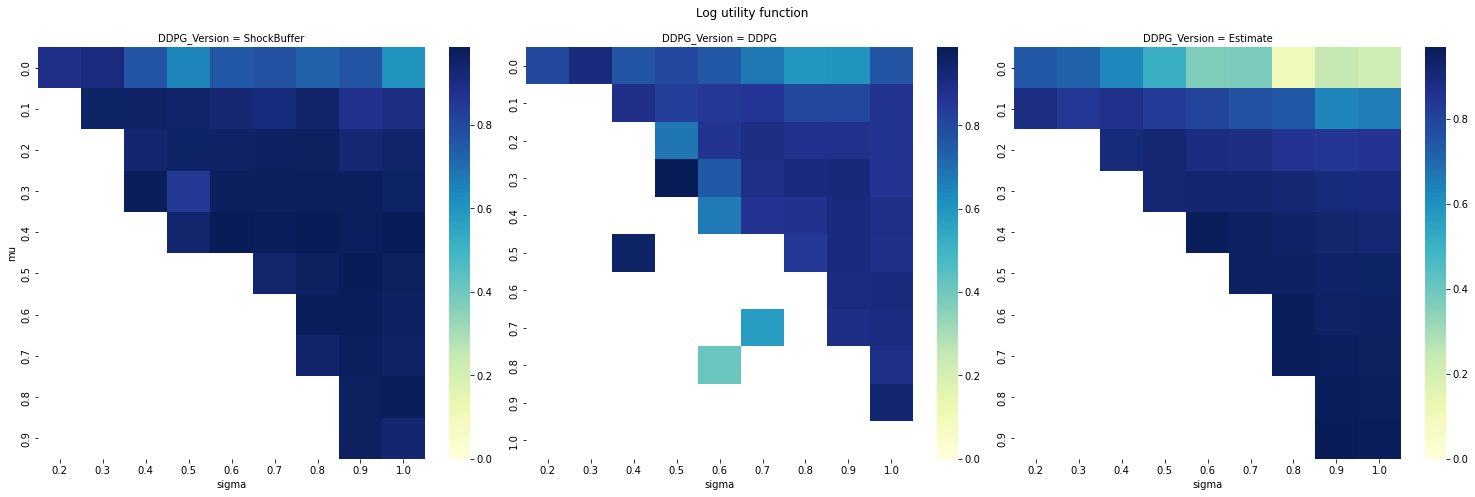
\includegraphics[width=1\textwidth,height=6cm]{figures/Results/Heatmaplog.png}
  \caption[Accuracy heat map - Log]{Accuracy heat map - Log utility} \label{fig:results:AHMLU}
\end{figure}
\begin{figure}[htpb]
    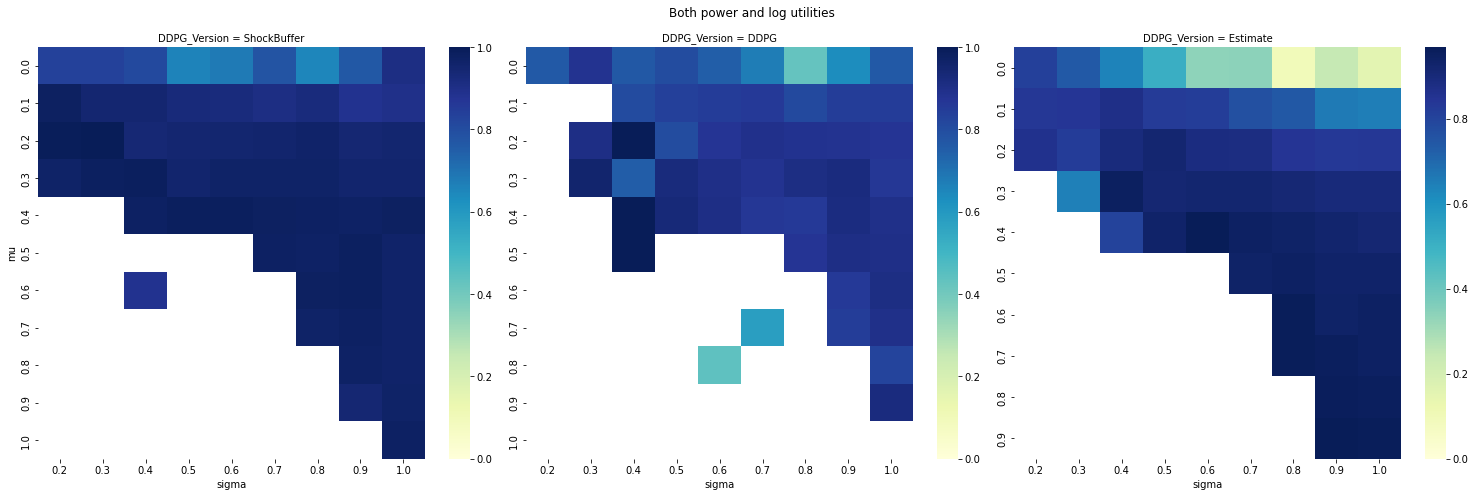
\includegraphics[width=1\textwidth,height=6cm]{figures/Results/heatmap_both.png}
  \caption[Accuracy heat map - All]{Accuracy heat map for both utility functions} \label{fig:results:AHMA}
\end{figure}

We see that Shock Buffer and Estimates have better accuracy in most of the regions in the heatmap. We also observe that there are no particular regions in the grid, where the accuracy is markedly different (for any of the algorithms). We do note that when $\mu$ is small, the accuracy is lower. However, the expected optimal action for both utility functions are directly proportional to $\mu$. Hence, when the optimal action value is also very small, the accuracy may be significantly impacted even for minor perturbations from the theoretical values.

\pagebreak

\subsection{Risk Aversion analysis for Power Utility}
We also analyzed with a number of values for $b$, the risk aversion factor for the power utility function.  We expect that as b approaches 1, the absolute losses should increase as the true optimal allocation $\pi^*$ also increases. 

The configuration for these experiments are shown in Table \ref{table:config_b}  and the results are shown in Figure \ref{fig:results:bA}.

\begin{table}[]
\caption{Configuration - Environment Analysis - Risk aversion} \label{table:config_b}
\begin{tabular}{||p{3cm}|p{2cm}||p{2cm}|p{2cm}||p{2cm}|p{2cm}||}
\hline
\textbf{Environment Parameter} & \textbf{Sampled values} &\textbf{DDPG}\linebreak \textbf{Parameter}& \textbf{Values} &\textbf{DDPG}\linebreak \textbf{Parameter} & \textbf{Values}\\
\hline

$\mu \in [0,1]$          & [0.07,0.955] & Version & DDPG, Shock Buffer, Estimates & Batch Size          & 1024 \\
\hline
$\sigma \in [0,1]$       & [0.1,1.0] & Grid Points &20 (Estimate)& Batch Size Growth & None \\
\hline
\Delta t          & 0.2 & Shock Buffer Size & 8 (Shock Buffer)& &\\
\hline
$v_0$        & 1 & Noise \linebreak  Decay       & Linear & & \\
\hline
Utility     & power  & Noise \linebreak  Scale       & 1 &&  \\
\hline
$\mathbf{b \in [-10,1) \backslash \{0\}}$           & \textbf{[-9,0.95]} & $\tau$& $5.10^{-4}$ && \\
\hline
            T&1  &$\tau$ decay         & Linear && \\
\hline
            $r_c$&0  & Buffer Length     & $10^{4}$ && \\
\hline
\end{tabular}
\end{table}


\begin{figure}[htpb]
    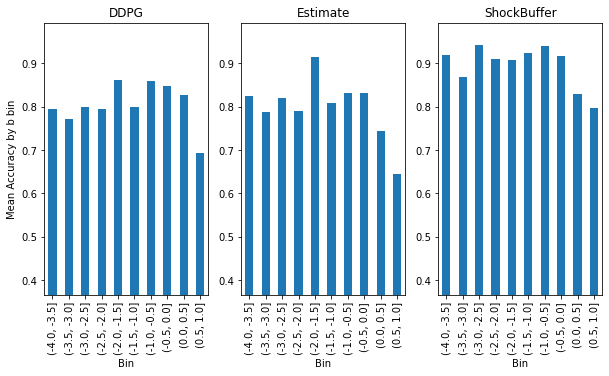
\includegraphics[width=1\textwidth,height=6cm]{figures/Results/bA.png}
  \caption[B Analysis]{Risk aversion analysis } \label{fig:results:bA}
\end{figure}



\section{DDPG Hyper Parameter Analysis}
\subsection{$\tau$ - Target Parameters Learning Rate}
The target network is updated periodically with the parameters from the main network. The rate, $\tau$ at which the target network is updated is controlled by a hyperparameter known as the target network learning rate. A low value for $\tau$ means that the target network parameters are updated slowly, which can help to stabilize the learning process. On the other hand, a high value for $\tau$ means that the target network parameters are updated quickly, which can lead to faster convergence but may also lead to instability in the learning process.  

\subsubsection{Adaptive tau}
 We can set $\tau$ to be high for faster convergence in the beginning of the experiments while reducing it gradually over time to stabilize the process. Sample plots from our experiments showing the representative effect is shown in the 
Figure \ref{fig:tau_analysis}. In the Tau\_Adaptive case, the initial value of $\tau$ is multiplied in  by the factor $(TotalEpisodes-currentEpisode)/TotalEpisodes$ before each update

\begin{figure}[!tbp]
  \centering
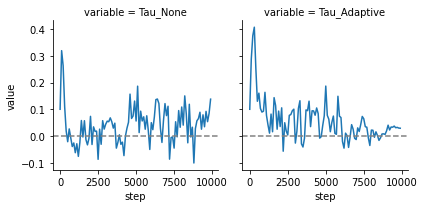
\includegraphics[width=1\textwidth,height=0.2\textheight]{figures/AdaptiveTau.png}
  \caption{$\tau$ analysis for 2 similar experiments}\label{fig:tau_analysis}
\end{figure}
\break
We tried to conduct experiments for studying the effects of adaptive $\tau$ based on the formula we earlier described. We present the configuration of these experiments in Table \ref{table:config_Tau} and the results in Figure \ref{fig:results:tau}
\begin{table}[]
\caption{Configuration - Tau Analysis} \label{table:config_Tau}
\begin{tabular}{||p{3cm}|p{2cm}||p{2cm}|p{2cm}||p{2cm}|p{2cm}||}
\hline
\textbf{Environment Parameter} & \textbf{Sampled values} &\textbf{DDPG}\linebreak \textbf{Parameter}& \textbf{Values} &\textbf{DDPG}\linebreak \textbf{Parameter} & \textbf{Values}\\
\hline

$\mu \in [0,1]$          & [0.07,0.955] & Version & DDPG, Shock Buffer, Estimates & Batch Size          & 1024 \\
\hline
$\sigma \in [0,1]$       & [0.1,1.0] & Grid Points &20 (Estimate)& Batch Size Growth & None \\
\hline
\Delta t          & 0.2 & Shock Buffer Size & 8 (Shock Buffer)& &\\
\hline
$v_0$        & 1 & Noise \linebreak  Decay       & Linear & & \\
\hline
Utility     & power  & Noise \linebreak  Scale       & 1 &&  \\
\hline
$b \in [-10,1) \backslash \{0\}$ & [-10,1) & $\tau$& $5.10^{-4}$ && \\
\hline
            &  & \textbf{Tau Decay}         & \textbf{None and Linear} && \\
\hline
            $r_c$&0  & Buffer Length     & $10^{4}$ && \\
\hline
\end{tabular}
\end{table}


\begin{figure}[!tbp]
     \subfloat[Box plot Analysis Tau ][Box plot analysis - $\tau$ ]{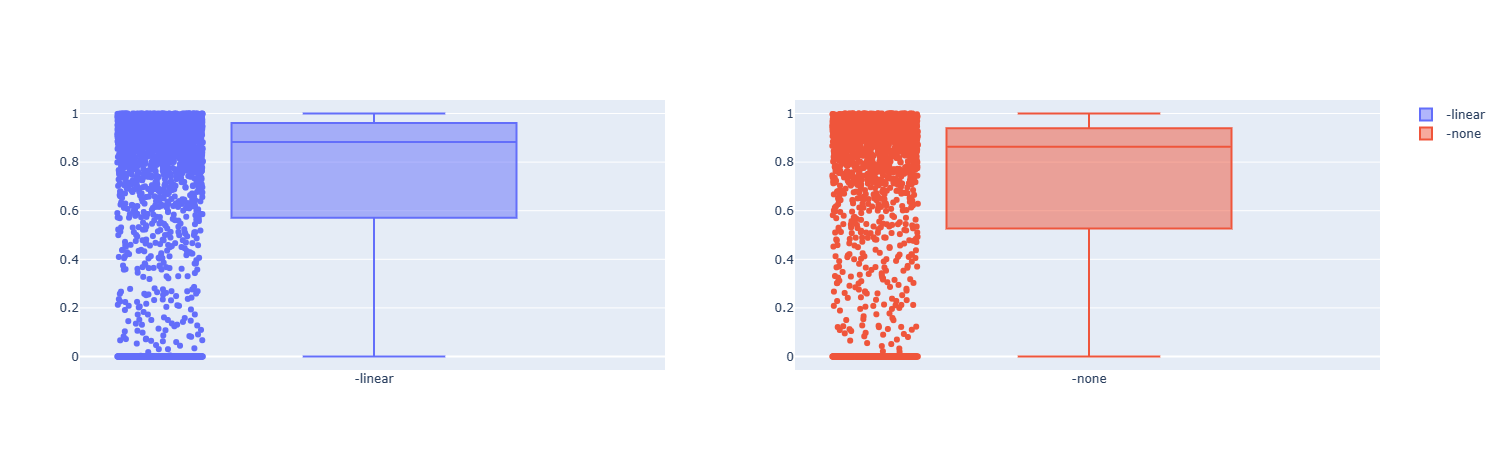
\includegraphics[width=1\textwidth,height=0.22\textheight]{figures/Results/Tau.png}}
  \vfill
  \subfloat[Table analysis Tau ][Table analysis  - $\tau$ ]{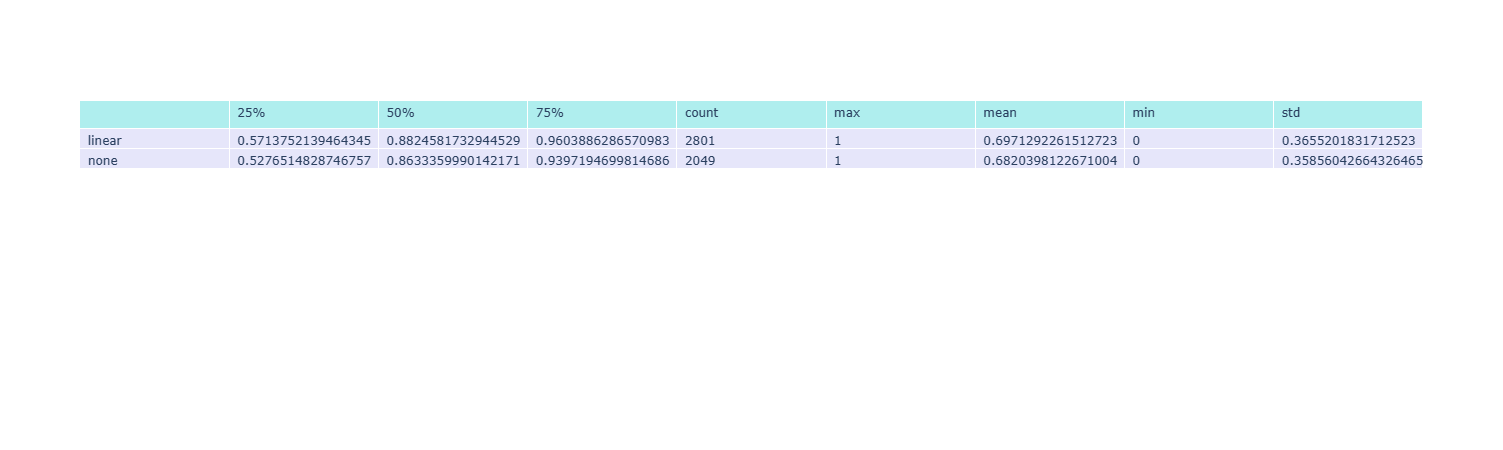
\includegraphics[width=1\textwidth,height=0.22\textheight]{figures/Results/Taudf.png}}
  
  \caption{ $\tau$ analysis}
  \label{fig:results:tau}
\end{figure}
 We noted that having an adaptive policy for tau decay has a positive effect in our experiments.
 \pagebreak
\subsection{Noise Process}

In our experiments, to model the exploration policy while arriving at the optimal action we used the Ornstein Uhlenbeck Process \cite{uhlenbeck1930} as stated in the original paper to generate correlated noise.
In the i-th training step, the noise level $X_i$ is updated recursively through the equation
\begin{equation}\label{equation:ounoise}
    X_i= (1-\kappa\Delta_N) X_{i-1}
    + \sigma_N \sqrt{\Delta_N}\mathcal{N},
\end{equation}

for positive constants $\kappa,\Delta_N,\sigma_N$  and $\mathcal{N} \sim \mathcal{N}(0,1)$.
In our experiments we set $\sigma_N = 0.2$ (volatility of the noise process). $\kappa = 0.15$ (rate at which $X$ reverts to the mean) and $\Delta_N=0.2$

For every call to the noise object specified in Algorithm \ref{alg:eventloop},we update the noise level as per (\ref{equation:ounoise}). Then the noise level is scaled according to an additional hyper parameter. Morever, we have another hyper parameter that decays the whole noise level as we progress on an experiment. Finally we add the resulting noise level to the estimated optimal action, $a^{\phi}$ which we compute at every step. This whole procedure is shown in Algorithm \ref{alg:NoisePolicy}.

\begin{algorithm}
\caption{Noise process - Hyper parameter tuning}
\label{alg:NoisePolicy}
\begin{algorithmic}[1]
\Require
\Statex $currentEpisode,TotalEpisodes$
\Statex $scale,decay$ \Comment{scale is a numeric hyperparameter, decay is a boolean hyperparameter to linearly decay the noise level }
\Statex $noiseLevel,\theta,\mu,\sigma,\Delta t$ \Comment{Parameters of the OU process, $\Delta t$ is the time step}
\Statex $currentEpisode,TotalEpisodes$

\Statex
\State  $noiseLevel \gets \left(
            noiseLevel 
            *(1-\kappa\Delta_N) 
    + \sigma_N \sqrt{\Delta_N}*StandardNormalVariable() 
        \right)$
\State Store $noiseLevel$
\State $decayFactor \gets 1$
\If{$decay = True$}
    \State $decayFactor = (TotalEpisodes-currentEpisode)/TotalEpisodes$
\EndIf
\State \Return {$decayFactor*scale*noiseLevel$}

\end{algorithmic}
\end{algorithm}

By increasing the $scale$  hyper parameter, we can control the exploration part in seeking the optimal action, and by setting $decay$ to True, we can achieve better convergence (while also allowing for high exploration in the beginning of the experiment). These effects are illustrated in Figure \ref{fig:noise_analysis}.

\begin{figure}[H]
  \centering
  \subfloat[Noise low ][Noise factor 0.1]{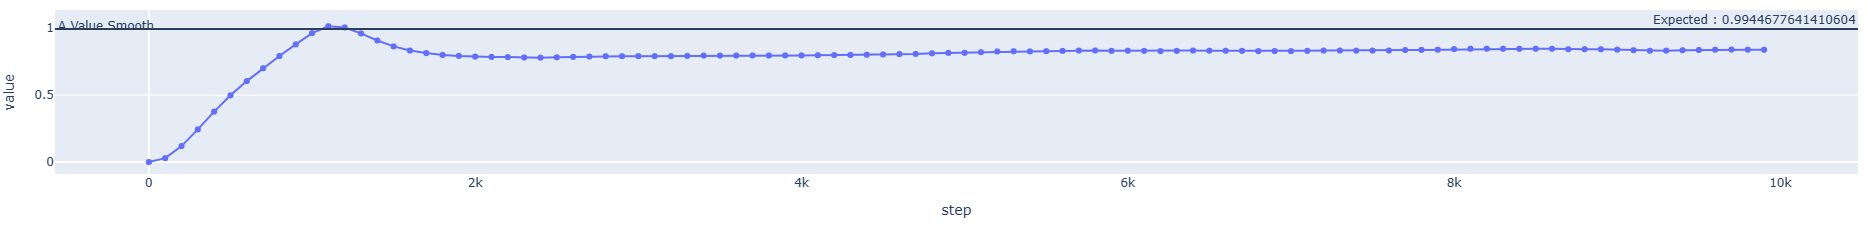
\includegraphics[width=1\textwidth,height=0.2\textheight]{figures/noise_scale_01.png}\label{fig:noise_low}}
  \vfill
  \subfloat[Noise high][Noise factor 5]{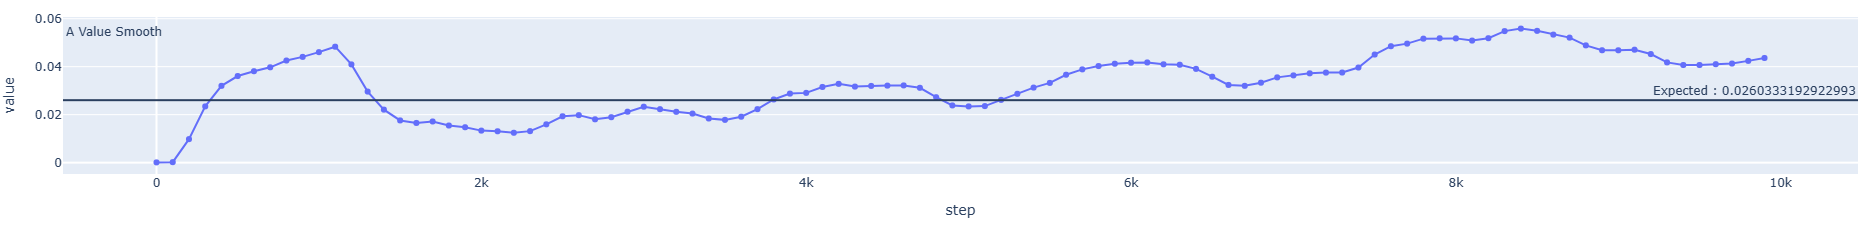
\includegraphics[width=1\textwidth,height=0.2\textheight]{figures/noise_high.png}\label{fig:noise_high}}
  \vfill
    \subfloat[Noise Adaptive][Adaptive noise]{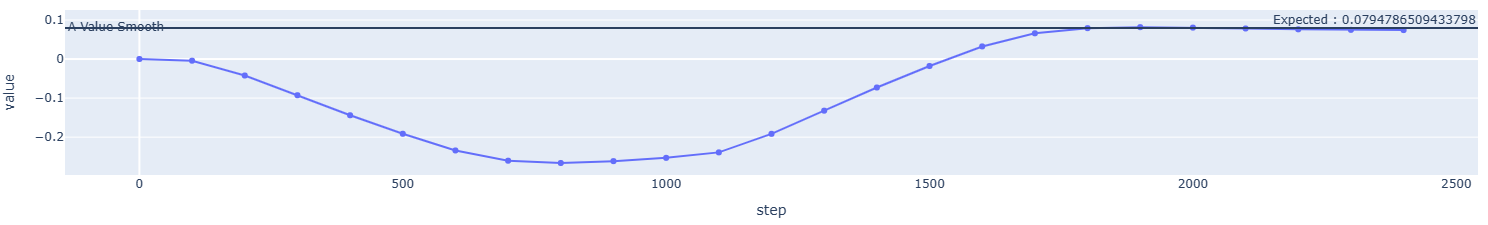
\includegraphics[width=1\textwidth,height=0.2\textheight]{figures/AdativeNoise.png}\label{fig:noise_adaptive}}
  \caption{Noise scale analysis to illustrate effects on convergence and accuracy}
  \label{fig:noise_analysis}
\end{figure}

We conducted a batch of experiments to study the effect of noise scale on the performance, the configuration of the experiments is shown in Table \ref{table:config_noise} and the corresponding results are shown in Figure \ref{fig:results:ns}.

\begin{table}[]
\caption{Configuration - Noise scale Analysis } \label{table:config_noise}
\begin{tabular}{||p{3cm}|p{2cm}||p{2cm}|p{2cm}||p{2cm}|p{2cm}||}
\hline
\textbf{Environment Parameter} & \textbf{Sampled values} &\textbf{DDPG}\linebreak \textbf{Parameter}& \textbf{Values} &\textbf{DDPG}\linebreak \textbf{Parameter} & \textbf{Values}\\
\hline

$\mu \in [0,1]$          & [0.02,0.42] & Version & Shock Buffer& Batch Size          & 1024 \\
\hline
$\sigma \in [0,1]$       & [0.35,0.98] & Grid Points &- & Batch Size Growth & None \\
\hline
\Delta t          & 0.2 & Shock Buffer Size & 8 (Shock Buffer)& &\\
\hline
$v_0$        & 1 & Noise \linebreak  Decay       & Linear & & \\
\hline
Utility     & power, log  & \textbf{Noise scale}       & \textbf{\{0.1,1,2,5\}} &&  \\
\hline
$b \in [-10,1) \backslash \{0\}$ & [-8.1,0.73] & $\tau$& $5.10^{-4}$ && \\
\hline
            T&1  &$\tau$ decay         & Linear && \\
\hline
            $r_c$&0  & Buffer Length     & $10^{4}$ && \\
\hline
\end{tabular}
\end{table}

\begin{figure}[H]
    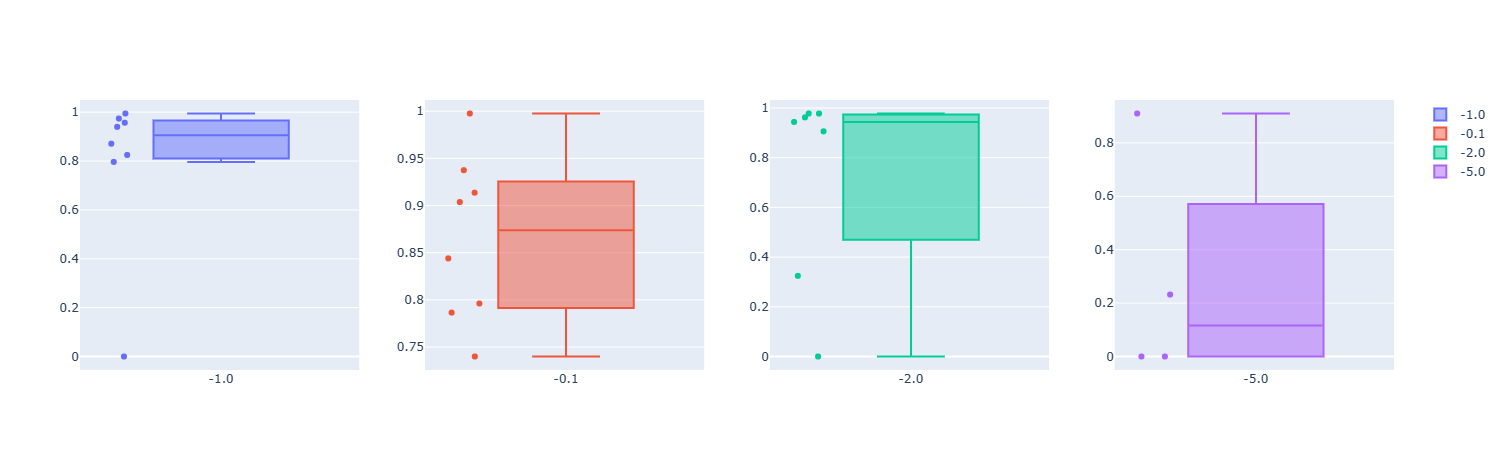
\includegraphics[width=1\textwidth,height=6cm]{figures/Results/NoiseScale.png}
  \caption[Noise scale]{Noise scale Analysis } \label{fig:results:ns}
\end{figure}

We noted that in our experiments having a higher or lower noise scale to increase/decrease our exploration generally did not improve our performance for the configuration we tested.
\pagebreak

\subsection{Episodes}
Typically, we would expect that as we increase the number of episodes, the algorithm should converge. If we observe that the algorithm does not converge it could be mainly because of 2 reasons in our set up (assuming $\tau$ is not decayed).
\begin{itemize}
    \item Approximation for the expectation in the equation (\ref{eq:BMO1}) is too inaccurate (which we discussed in depth in earlier Chapters \ref{chapter:ShockBuffer} and \ref{chapter:Estimates})
    \item The Bellman equation cannot be fitted in a stable manner 
\end{itemize}
\begin{figure}[!tbp]
     \subfloat[Good Covergence ][Good convergence ]{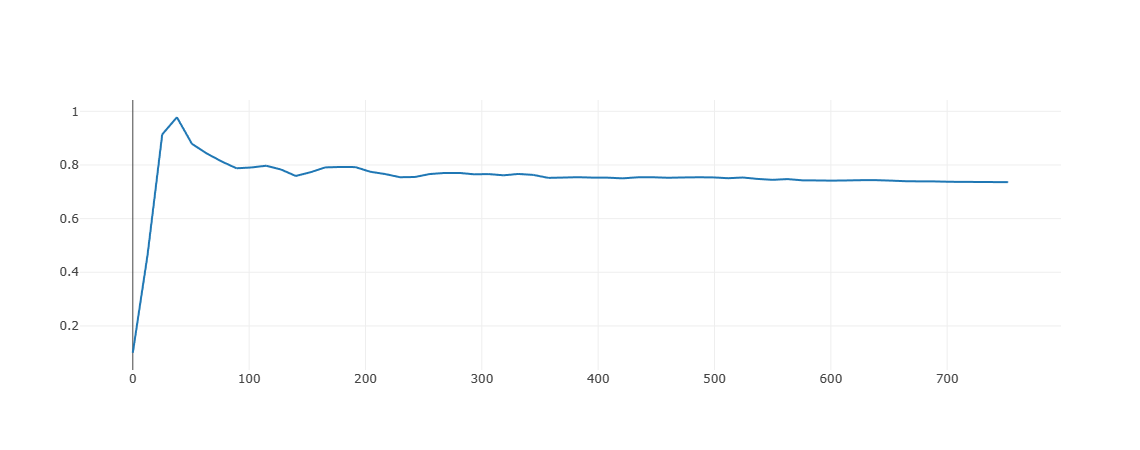
\includegraphics[width=1\textwidth,height=0.22\textheight]{figures/Results/GoodConvergence.png}}
  \vfill
  \subfloat[No convergence ][No Convergence ]{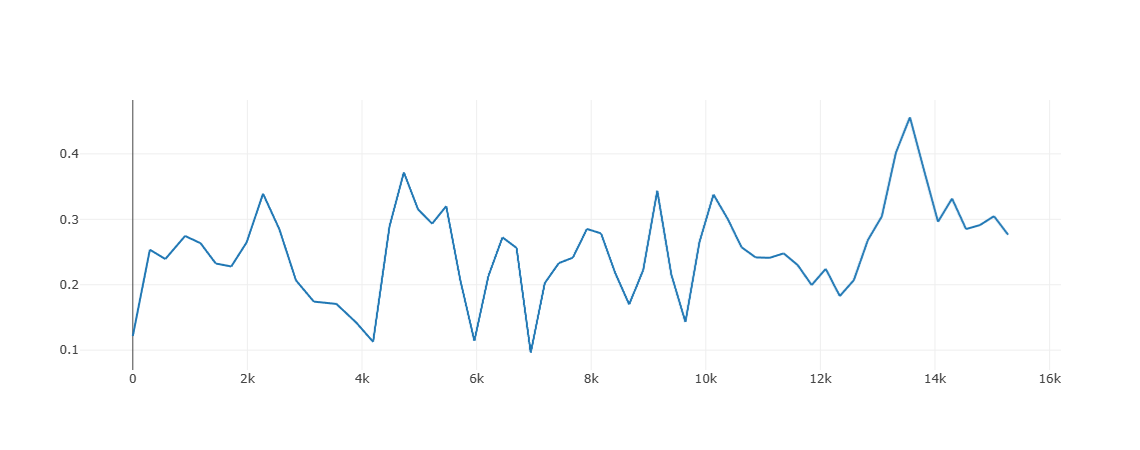
\includegraphics[width=1\textwidth,height=0.22\textheight]{figures/Results/NoConvergence.png}}
  
  \caption{ Episode hyperparamter - to show the solution either converging  or not in our experiments}
  \label{fig:episdode_analysis}
\end{figure}
\pagebreak
When we do not decay $\tau$, or noise over time, we see both good convergence and poor convergence in our experiments. This is shown in Figure \ref{fig:episdode_analysis} - all other parameters of the 2 experiments except $\mu$ and $\sigma$ were identical and yet the convergence was quite different.

We conducted experiments to analyse the effects of the number of episodes. The configuration of these experiments are provided in Table \ref{table:config_episodes} and the results in Figure \ref{fig:results:episodes_analysis_all}.
\begin{table}[]
\caption{Configuration - Number of episodes analysis } \label{table:config_episodes}
\begin{tabular}{||p{3cm}|p{2cm}||p{2cm}|p{2cm}||p{2cm}|p{2cm}||}
\hline
\textbf{Environment Parameter} & \textbf{Sampled values} &\textbf{DDPG}\linebreak \textbf{Parameter}& \textbf{Values} &\textbf{DDPG}\linebreak \textbf{Parameter} & \textbf{Values}\\
\hline

$\mu \in [0,1]$          & [0.016,0.62] & Version & Shock Buffer and Estimates& Batch Size          & 1024 \\
\hline
$\sigma \in [0,1]$       & [0.27,0.98] & Grid Points &20 (Estimates) & Batch Size Growth & None \\
\hline
\Delta t          & 0.2 & Shock Buffer Size & 8 (Shock Buffer)&\textbf{ Episodes} &\textbf{\{}$\mathbf{2.10^4,4.10^4,}$ \lineabreak $ \mathbf{8.10^4}$\textbf{\}}\\
\hline
$v_0$        & 1 & Noise \linebreak  Decay       & Linear & & \\
\hline
Utility     & power, log  & Noise \linebreak  Scale       & 1.0 &&  \\
\hline
$b \in [-10,1) \backslash \{0\}$ & [-7,0.6] & $\tau$& $5.10^{-4}$ && \\
\hline
            T&1  &$\tau$ decay         & Linear && \\
\hline
            $r_c$&0  & Buffer Length     & $10^{4}$ && \\
\hline
\end{tabular}
\end{table}



    \begin{figure}[H]
  \subfloat[Table analysis ][Table analysis - number of episodes ]{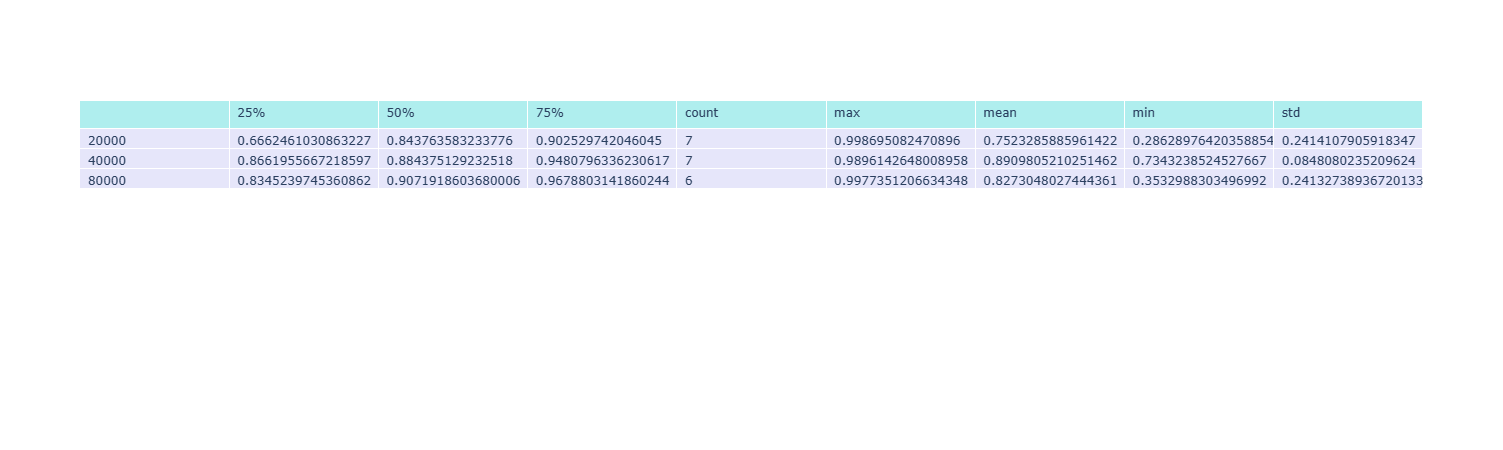
\includegraphics[width=1\textwidth,height=0.22\textheight]{figures/Results/episodes_analysis.png}}
  
  \caption{ Episodes analysis}
  \label{fig:results:episodes_analysis_all}
\end{figure}

We see that when we increase the number of episodes, accuracy does increase (albeit only marginally). For Estimates we did not see any improvement as we increase the number of episodes. When we inspected individual plots, we find out that convergence (even if not to the optimal action) happens fairly early during training. 


\section{Robust Simulations} \label{section:rs}



After our initial experiments, we observed 2 key points.
\begin{itemize}
    \item Increasing the number of episodes only marginally increases the accuracy. We observed the Q loss decreased with episodes but the optimal action was not necessarily maximized.
    \item Shock Buffer and Estimates  performed better in almost all aspects compared to DDPG.
\end{itemize}
So coming up with more accurate expectations in Equation (\ref{eq:BMO1}) helped a long way for having robust simulations. We used this idea and tried to build better estimates by the following methods.

\subsection{Estimates}
We conducted 2 kinds of experiments. 
\begin{itemize}
\item
We created 2 sets of partitions -  coarse and fine over $-\inf,\inf$. We used the fine ones from -0.5 to 0.5 roughly and coarse ones outside of that interval. The reason behind this idea was to build different (and better) partition sets for estimates that would better converge to the expected value. 
\item
\textit{Adaptive partition strategy}: We started  off with very fine partitions (around 200) to begin with and then increased over time.
\end{itemize}
However we noted that both these experiments did not improve the accuracy by much. Then we decided on a brute force solution and merely increased the number of grid points, i.e "m", to a very high number - increased from 20 to 1000. We kept the number of episodes to 2500 as we observed that convergence happens rapidly in Estimates. We also built our solution on GPUs to help us cope with the memory constraints such a configuration would entail.

\subsection{Shock Buffer}

We followed a very similar strategy for Shock Buffer. However, as we observed that Shock Buffer took longer to converge, we increased the number of episodes to 6000, while increasing the mini batch size $m=B_p$ for log returns from 20 to 1000.
\pagebreak
\subsection{Results}
We then ran these configurations on both power and log utility functions and repeated the experiment under different market parameters. We display the configuration of these experiments in Table \ref{table:config_env} and the results in Figure \ref{fig:results:M}.

\begin{table}[]
\caption{Configuration - M Analysis} \label{table:config_env}
\begin{tabular}{||p{3cm}|p{2cm}||p{2cm}|p{2cm}||p{2cm}|p{2cm}||}
\hline
\textbf{Environment Parameter} & \textbf{Sampled values} &\textbf{DDPG}\linebreak \textbf{Parameter}& \textbf{Values} &\textbf{DDPG}\linebreak \textbf{Parameter} & \textbf{Values}\\
\hline

$\mu \in [0,1]$          & [0.07,0.955] & Version & DDPG, Shock Buffer, Estimates & Batch Size          & 1024 \\
\hline
$\sigma \in [0,1]$       & [0.1,1.0] & Grid Points &\textbf{1000} (Estimates)& Batch Size Growth & None \\
\hline
\Delta t          & 0.2 & Shock Buffer Size & \textbf{1000} (Shock Buffer)& Episodes& \textbf{Estimates: 2500   \lineabreak Shock Buffer: 6000 }\\
\hline
$v_0$        & 1 & Noise \linebreak  Decay       & Linear & & \\
\hline
Utility     & power and log & Noise \linebreak  Scale       & 1 &&  \\
\hline
$b \in [-10,1) \backslash \{0\}$ & [-9.0,0.95] & $\tau$& $5.10^{-4}$ && \\
\hline
            T&1  &$\tau$ decay         & Linear && \\
\hline
            $r_c$&0  & Buffer Length     & $10^{4}$ && \\
\hline
\end{tabular}
\end{table}
\begin{figure}[!tbp]
     \subfloat[Box plot Analysis M ][Box plot analysis - m ]{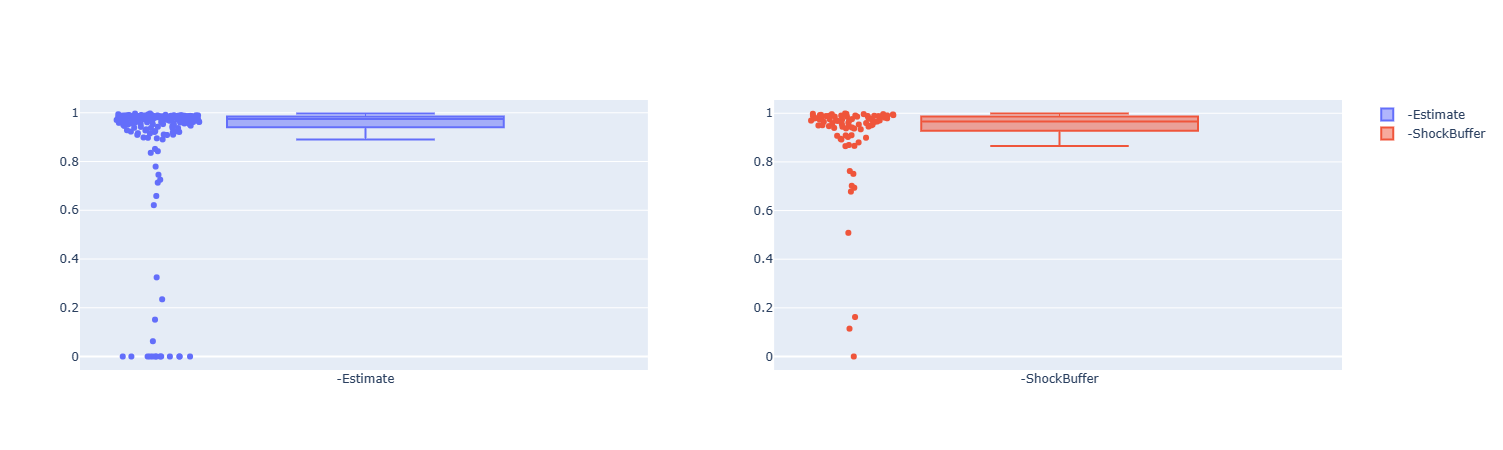
\includegraphics[width=1\textwidth,height=0.22\textheight]{figures/Results/Accuracy_M.png}}
  \vfill
  \subfloat[Table analysis M ][Table analysis estimates - m]{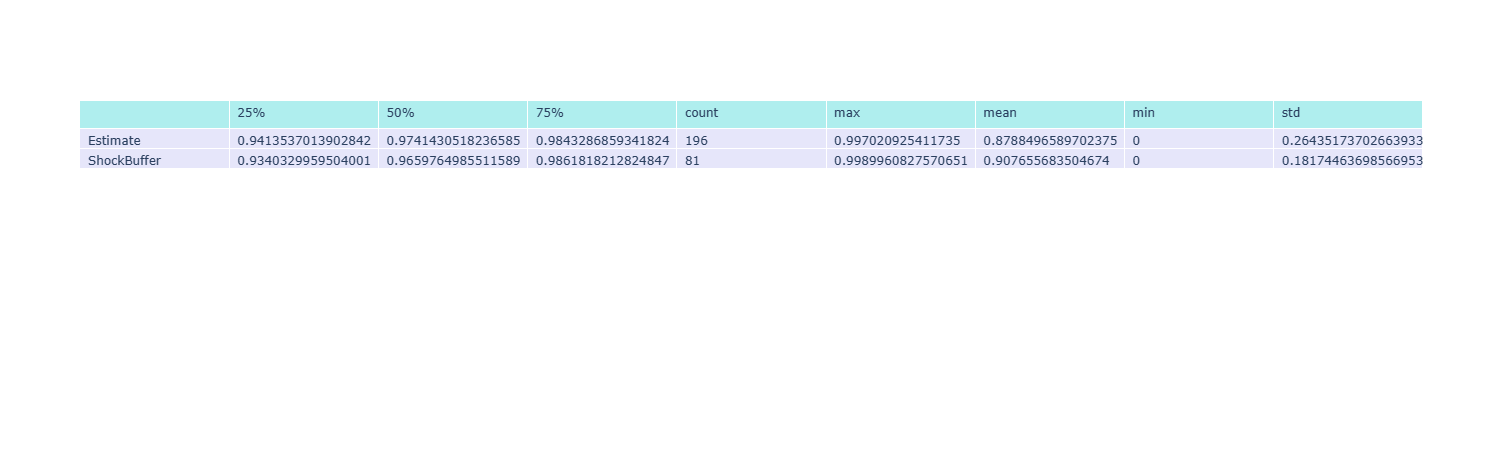
\includegraphics[width=1\textwidth,height=0.22\textheight]{figures/Results/Accuracy_M_df.png}}
  
  \caption{ $m$ analysis}
  \label{fig:results:M}
\end{figure}


We observed that this version of both these algorithm performed comparatively better, even we decreased $\Delta t$ from 0.2 to 0.01. The results for $\Delta t = 0.01$ (other configuration parameters are the same) are shown in Figure \ref{fig:results:ML}


\begin{figure}[!tbp]
     \subfloat[Box plot Analysis M (large timesteps) ][Box plot analysis m ]{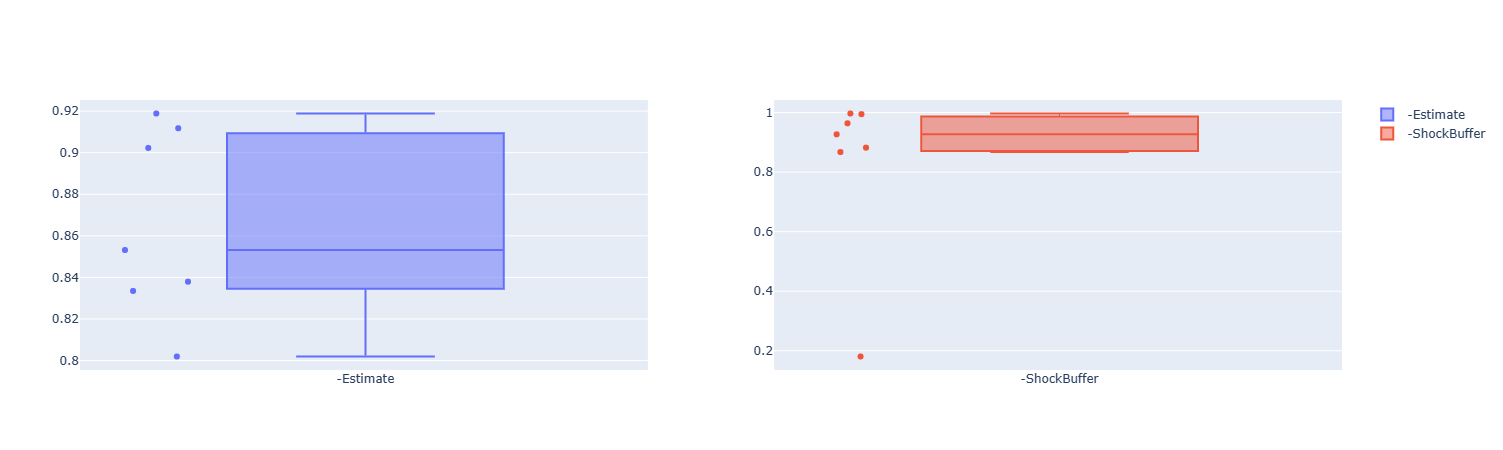
\includegraphics[width=1\textwidth,height=0.22\textheight]{figures/Results/Accuracy_M_long.png}}
  \vfill
  \subfloat[Table analysis M (large timesteps)][Table analysis estimates - m ]{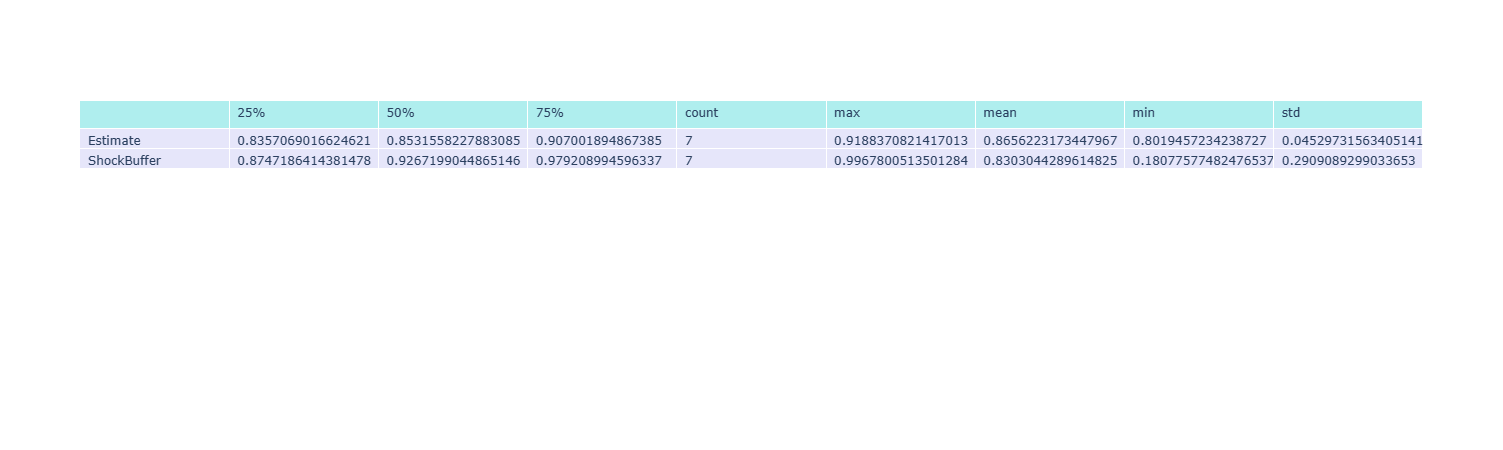
\includegraphics[width=1\textwidth,height=0.22\textheight]{figures/Results/Accuracy_M_df_long.png}}
  
  \caption{ $m$ analysis - $\Delta t$ - 0.01}
  \label{fig:results:ML}
\end{figure}

These results are much better than our initial analysis. It does appear that Shock Buffer is better compared to the Estimates. However, we also note that Estimates is much faster (around 3 times faster) than Shock Buffer in the above set up.  Further, we notice that as we keep increasing the number of grid points, the accuracy of Estimates also increases. Hence, Estimates, in a sense, can be regarded as equivalent to the Shock Buffer. 

Another interesting pattern we found was that Estimates performed much better for log utility functions than for power utility functions. However, we could not find such a pattern for  Shock Buffer. This pattern is captured in Figure \ref{fig:results:EstimatesU2} and \ref{fig:results:SBU2}

\begin{figure}[!tbp]
     \subfloat[Box plot Analysis - Estimates for Utility functions  ][Box plot Analysis - Estimates for log and power utility functions ]{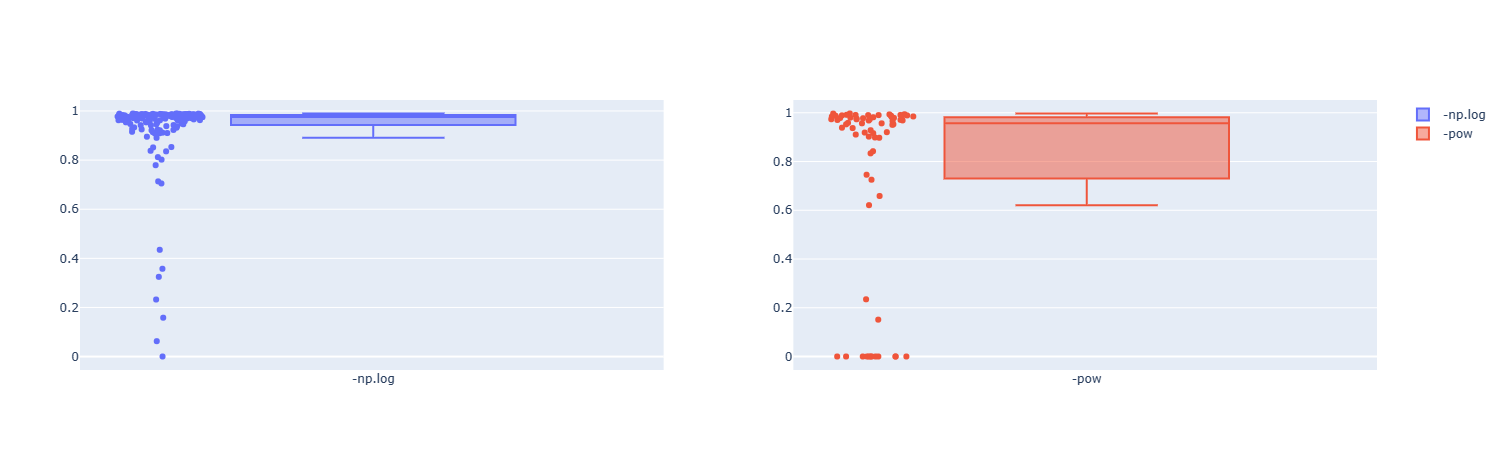
\includegraphics[width=1\textwidth,height=0.22\textheight]{figures/Results/Accuracy_MEU2.png}}
  \vfill
  \subfloat[Table analysis - Estimates for Utility functions ][Table analysis Estimates for log and power utility functions ]{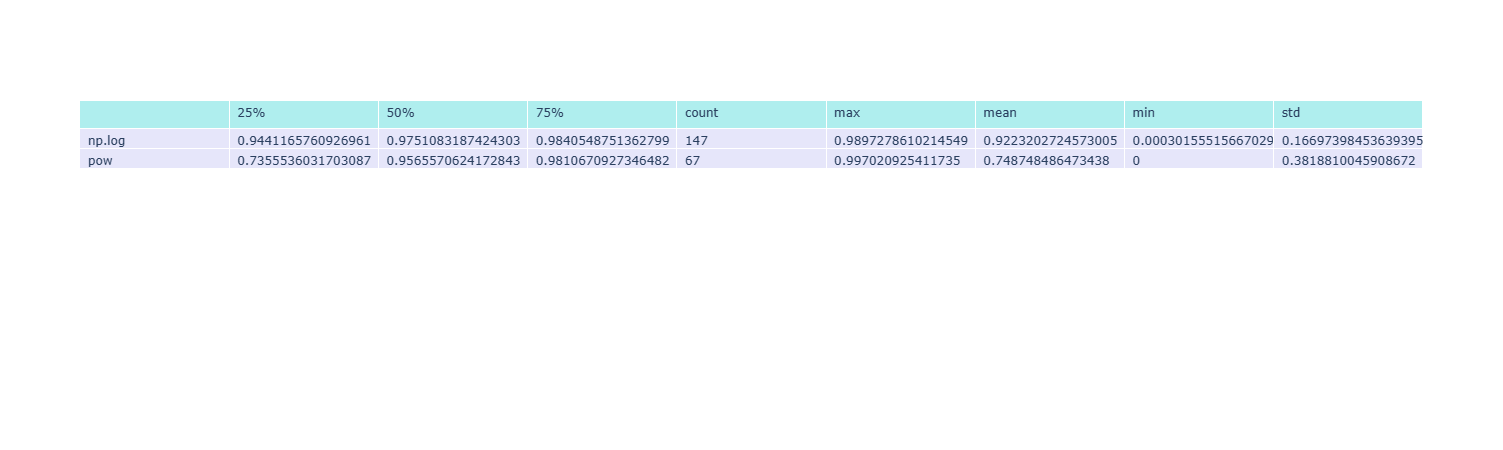
\includegraphics[width=1\textwidth,height=0.22\textheight]{figures/Results/Accuracy_MEU2_df.png}}
  
  \caption{ Utility functions analysis - Estimates}
  \label{fig:results:EstimatesU2}
\end{figure}


\begin{figure}[!tbp]
     \subfloat[Box plot Analysis - Shock Buffer for Utility functions  ][Box plot Analysis - Shock Buffer for log and power utility functions ]{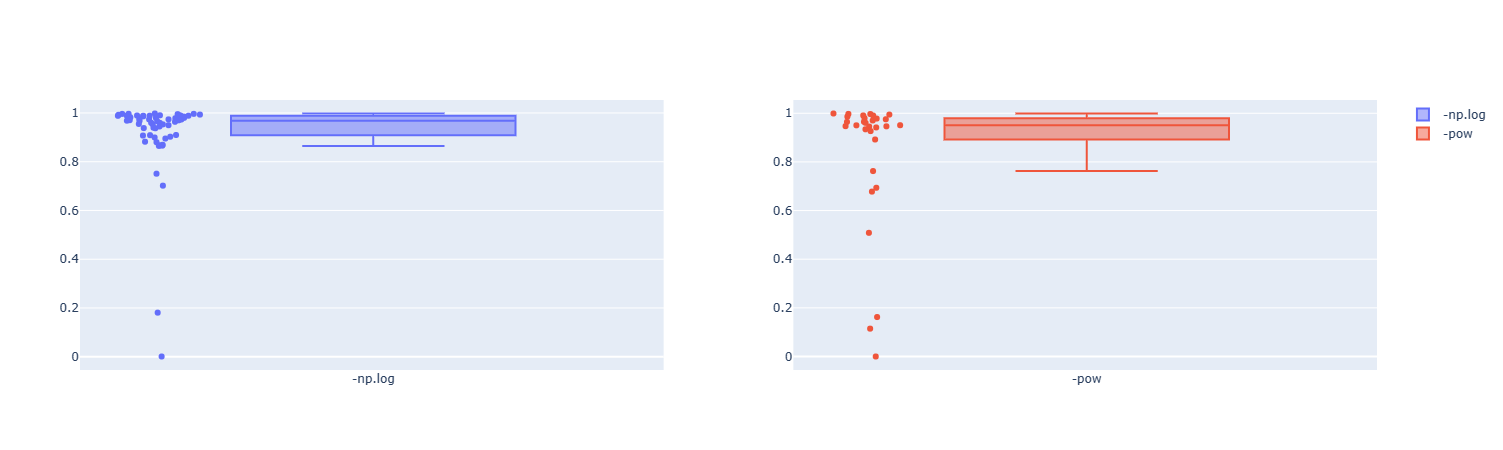
\includegraphics[width=1\textwidth,height=0.22\textheight]{figures/Results/Accuracy_MEU2SB.png}}
  \vfill
  \subfloat[Table analysis - Shock Buffer for log and power utility functions ][Table analysis Shock Buffer for log and power utility functions ]{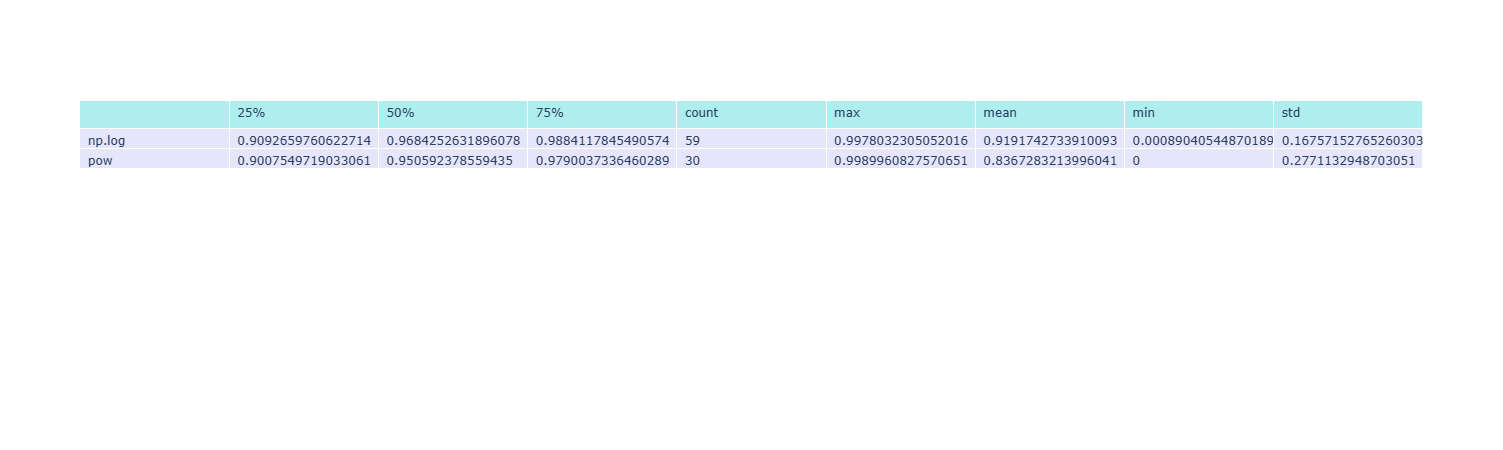
\includegraphics[width=1\textwidth,height=0.22\textheight]{figures/Results/Accuracy_MEU2_dfSB.png}}
  
  \caption{ Utility functions analysis - Shock Buffer}
  \label{fig:results:SBU2}
\end{figure}









\chapter{Conclusion and Future Work}\label{chapter:11_Future_Work}
In this final brief chapter, we summarize the results we obtained in the previous Chapter \ref{chapter:Results}, and recommend our best models we observed in our experiments. We finally conclude by listing some of the future work that could be done extending this framework to other class of problems and some improvements that could be made to the existing software architecture.

\section{Conclusion}


Based on the results we obtained in the previous chapter, we noticed that the most important factor for improving the accuracy and robustness of our results was to improve the estimation for the expectation defined in Equation \ref{eq:BMO1}. This can be achieved by increasing the shock buffer batch size in Shock Buffer and number of grid points in Estimates (commonly referred as $m$ in both the methods). Increasing the number of episodes was the next most important factor that increased the accuracy, especially observed in Shock Buffer and DDPG. Adaptive $\tau$ also marginally improved the accuracy in our experiments.  These results are further summarized in Table \ref{table:summary}.

In this sense, we recommend both Shock Buffer, and Estimates as our preferred algorithms. The configuration described in Section \ref{section:rs} (for both methods) yielded the most promising results in our experiments. However, we also believe that one could achieve even better accuracy and convergence speed by further increasing the factor $m$. 


\begin{table}
\begin{tabular}{ ||p{2cm}|p{2cm}|p{3cm}|p{7cm}||  } 
 \hline
 \hline
\textbf{Parameter}& \textbf{Impact} &\textbf{DDPG Version}&\textbf{Comment}\\
 \hline
 Stable estimate for expectation (\ref{eq:BMO1})   & High    &  Shock Buffer and Estimates & Computing stable estimates of expectation in the Bellman equation has a very positive impact on the accuracy. \\
 \hline
   Number of grid points   & High    &  Estimates & Increasing partitions to find the expected value of future Q values has a very positive effect on accuracy.\\
 \hline
  
   Batch size of log returns   & High    &  Shock Buffer & Increasing batch size of log shock returns to find the expected value of future Q values has a very positive effect on accuracy.\\
   \hline
   Batch size of state, action tuples   & Medium    &  All & Increasing batch size increases accuracy but only up to a level. Adaptive batch size marginally improves accuracy.\\
   \hline
   \tau   & Medium    &  All & Adaptive $\tau$ marginally improves accuracy, and convergence.\\
  \hline
   Noise scale   & Low    &  All & Did not significantly improve accuracy.\\
   \hline
    Number of episodes & Medium & All & \textbf{Estimates}: Did not impact accuracy after a rapid and an early converging level. \linebreak
    \textbf{Shock Buffer}: Impacted the accuracy considerably.  \\
    \hline
    Model parameters & None & All & Did not markedly notice domains of model parameters that impacted performance or convergence time.\\
    \hline
    Time discretization \Delta t & High & All & Accuracy and convergence time is proportional to \Delta t. \\
    
 \hline
 
\end{tabular}
\caption{\label{table:summary}Summary of results - Qualitative analysis}
\end{table}
\pagebreak
\section{Future Work}
Our study was very theoretical in which we generated observations from a model distribution. It was also a very simplistic problem with just 1 risky and 1 riskless asset. The utility functions we considered were also designed in such a way that the optimal allocation strategy could be explicitly derived and were independent from the time horizon in the experiments. The model distribution itself was very simple - a Black Scholes model with known mean and variance of the risky asset. The riskless rate was also assumed to be 0.

So considering all the discussed simplifications it is very obvious the tremendous scope and expansion of the current effort.
\begin{itemize}
    \item \textbf{Model Distribution}
    
    First of all we can build a slightly more complex environment. For instance instead of a Black Scholes environment, we can use a Heston environment \cite{Heston1993} where the volatility of the risky asset changes over time. There is also no limit on extending the environment by adding more parameters and increasing the complexity of the environment.
    \item \textbf{Empirical Data}
    
    We did not use actual returns that were observed in real markets to generate our optimal actions. A problem with using empirical real data is that we have only one realization. We can also build a capital market model and generate complex forward looking simulations of assets based on such a model. The problem with having such complex models is that our actor and critic may no longer be expressive and accurate enough to capture the underlying model.
    
    \item \textbf{Actor and Critic }

    Our actor and critic were actually parametrized versions of the theoretical values of Q and A values respectively. In essence, we almost supplied the exact answer to our experiments and just caliberated the parameters in those functions using DDPG. There are various improvements that can be done in this setting.
    \begin{itemize}
        \item \textbf{Generic expected forms of the solution}

        In many cases, we cannot find out or find out only numeric solutions of Q and A value functions. They are the real applications of this setting as we can feed in forms of our expected solution without explictly stating the actual form. The challenge then will be to understand if indeed the final solution is the optimal solution and also arriving at the generic form itself may be a challenge.

        \item \textbf{Generic forms with neural network}

        We can start off with the same set up as in the previous case, but infer the parameters of the generic function using deep neural networks. In addition to the usual performance related challenges,  convergence time, simulations needed, architecture of the neural network and other neural network related problems such as regularization, over fitting etc. are some of the other factors one must consider.

        \item \textbf{Mismatched functions}

        We can deliberately try to give mismatched functions to Q and A value functions and then understand how those functions capture information.
    \item \textbf{Multi-asset setting}

    We only discussed a simple setting with 1 risky asset in this problem. We can easily extend this to a multi-asset problem with a possibly time-changing correlation matrix between them. Such a setting would further challenge the robustness and the scalability of the developed algorithms.
    
    \item \textbf{Utility functions}

    We considered only 2 utility functions which are concave in the problem domain and functions in which the optimal action values were independent of the time axis. We can relax these rigid assumptions and can conduct further studies on many other utility functions.
    \end{itemize}
    \item \textbf{Software Architecture}

    The proposed architecture also could be improved, with better visualization, tracking and deployment suites. Most of what we implemented were custom built and tightly coupled with what we needed. A more thorough study on each of these aspects can be made.
    \begin{itemize}
        \item 
    
    \textbf{Distributed deployment} 
    
    We did not build any deployment pipelines over the cloud such as having a managed kubernetes cluster. Such a deployment could widely improve our abilities to conduct vast number of experiments over the problem domain
    \item \textbf{DAG for tensorflow}
    
    We did not exploit lazy evaluation and constructing directed acyclic graphs in tensorflow to speed up our computation. This would result in a major performance improvement in terms of speed.

    
    \item \textbf{Tensorboard} 
    
    We used MLFLow to track our experiments. We could have experimented with other visualization tools such as tensorboard \cite{tensorboard} and build better visualization charts.

    
    \item \textbf{Testing} 
    
    Our ML model is not integrated with any test suite to generate test cases and  check the validity of our experiments. Going forward this could be one crucial piece to quickly prototype and implement new features while conducting regression tests \cite{howden1978} on the validity of existing functionalities. 
  
    \end{itemize}
    
\end{itemize}





% TODO: add more chapters here



\microtypesetup{protrusion=false}
\listoffigures{}
\listoftables{}
\microtypesetup{protrusion=true}
\printbibliography{}

\end{document}
